\documentclass[11pt,a4paper,english]{article}
\usepackage[titletoc, title]{appendix}
\usepackage{amsmath}
\usepackage{amssymb}
\usepackage{bm}
\usepackage{array}
\usepackage{babel}
\usepackage{bbding}
\usepackage{color}
\usepackage[normal]{caption}
\usepackage{subcaption}
\usepackage{epsfig}
\usepackage{graphicx}
\usepackage{pdflscape}
%\usepackage{multirow}
\usepackage{psfrag}
\usepackage{proofapnd}
\usepackage[round]{natbib}
%\usepackage{bbm}
%\usepackage[T1]{fontenc}
%\usepackage[normal]{caption2} % for caption
\usepackage{rotating}
\usepackage[margin=2cm]{geometry} % for the same margin
\usepackage{latexsym}
%\usepackage{subfig}
\usepackage{setspace}
\usepackage{slashbox}
\usepackage{enumitem}
\usepackage{booktabs}
\usepackage{tabularx}
\usepackage{longtable,booktabs}

\setlist[itemize]{leftmargin=*}
\setlist[description]{leftmargin=*}

%\setlength{\topmargin}{0.0 in} \setlength{\textwidth}{6in}
%\setlength{\oddsidemargin}{0.5in}
%\setlength{\evensidemargin}{-0.01in} \setlength{\textheight}{9in}
\captionsetup{font={onehalfspacing,small}, labelfont=bf}

\title{\LARGE \bf Hedging Futures with Spectral Risk Measures}
%\author{
%	\begin{tabular}[t]{ccc}
%		Lu, Meng-Jou\thanks{Corresponding author. 
%			Department of Information and Finance
%			Management, Institute of Finance and Institute of Information
%			Management, National Chiao-Tung University, No.1001 Daxue Rd,
%			Hsinchu City, Taiwan. Ladislaus von Bortkiewicz Chair of Statistics,
%			Humboldt--Universit\"{a}t zu Berlin, C.A.S.E. -- Center for
%			Applied Statistics and Economics, Unter den Linden 6, 10099 Berlin, Germany.
%     E-mail: \texttt{mangrou@gmail.com}.}
%		 \and\and Nguyen, Phuong Anh   
%		\thanks{Department of Finance and Banking, School of Business, International University-VNUHCM, Ho Chi Minh City, Vietnam. E-mail:
%			\texttt{npanh@hcmiu.edu.vn}. }
%			\and\and  H\"{a}rdle, Wolfgang Karl
%			\thanks{Ladislaus von Bortkiewicz Chair of Statistics,
%				Humboldt--Universit\"{a}t zu Berlin, C.A.S.E. -- Center for
%				Applied Statistics and Economics, Unter den Linden 6, 10099 Berlin, Germany. Sim Kee Boon Institute for
%				Financial Economics, Singapore Management University
%				Administration Building, 81 Victoria Street, 188065 Singapore. The Wang Yanan Institute for Studies in Economics, Xiamen University. 
%				E-mail: \texttt{haerdle@hu-berlin.de}. }
%	\end{tabular}
%}
\date{This version: \today}
%%%%%%%%%%%%%%%%%%%%%%%%%%%%%%%%%%%%%%%%%%%%%%%%%%%%%%%%%%%%%%%%%%%%%%%%%%%%%%%%%%%%%%%%%%%%%%%%
\renewcommand{\baselinestretch}{1.2}
%\newcommand{\indicator}{$1{\hskip -2.5 pt}\hbox{I}$}
\newcommand{\indicator}{I}
\input{definitions}

\begin{document}

\newtheorem{lemma}{Lemma}
\newtheorem {proposition}[lemma]{Proposition}
\newtheorem {corollary}{Corollary}
\newtheorem {theorem}{Theorem}
\newtheorem{claim}[lemma]{Claim}
\newtheorem{comment}[lemma]{Comment}
\newtheorem{example}[lemma]{Example}
\newtheorem{fact}[lemma]{Fact}
\newtheorem{defn}[lemma]{Definition}
\newtheorem{exercise}{Exercise}[section]

\newtheorem{programming}[exercise]{Programming assignment}
\newenvironment{proof}{{\flushleft\textbf{\textsl{Proof.\ \ }}}}{\hfill{\hfill\rule{2mm}{2mm}}}
\pagenumbering{arabic}
\maketitle
%%%%%%%%%%%%%%%%%%%%%%%%%%%%%%%%%%%%%%%%%%%%%%%%%%%%%%%%%%%%%%%%%%%%%%%%%%%%%%%%%%%%%%%%%%%%%%%
\begin{abstract}
\footnotesize{ We investigate different methods of hedging cryptocurrencies with Bitcoin futures.
The introduction of derivatives on Bitcoin, in particular the launch of futures contracts on CME in December 2017,
allows for hedging exposures on Bitcoin and cryptocurrencies in general.
Because of volatility swings and jumps in Bitcoin prices, the traditional variance-based approach to obtain the hedge ratios is infeasible.
The approach is therefore generalised  to various risk measures, such as value-at-risk ,expected shortfall and spectral risk measures,
and to different copulas for capturing the dependency between spot and future returns, such as the Gaussian, Student-$t$,
NIG and Archimedean copulas. Various measures of hedge effectiveness in out-of-sample tests give insights in the practice of hedging Bitcoin and the CRIX index,
a cryptocurrency index. This is joint work with Meng-Jou Lu (Asian Institute of Digital Finance Credit Research Initiative,
National University of Singapore, Singapore) and Francis Liu (Berlin School of Economics and Law, Humboldt University Berlin).\\

\noindent {\bf JEL classification:}  \\
\noindent {\bf Keywords:} Portfolio Selection, Spectral Risk Measurement,  Coherent Risk}\pagestyle{empty}\\
\end{abstract}


\clearpage
%%%%%%%%%%%%%%%%%%%%%%%%%%%%%%%%%%%%%%%%%%%%%%%%%%%%%%%%%%%%%%%%%%%%%%%%%%%%%%%%%%%%%%%%%%%%%%%%%%%%%%%%%%%%%%%%%%%%%%%%%%%%%%%%%%%%%%%%%%%%%%%%%%%%%%
%%%%%%%%%%%%%%%%%%%%%%%%%%%%%%%%%%%%%%%%%%%%%%%%%%%%%%%%%%%%%%%%%%%%%%%%%%%%%%%%%%%%%%%%%%%%%%%%%%%%%%%%%%%%%%%%%%%%%%%%%%%%%%%%%%%%%%%%%%%%%%%%%%%%%%
\section{Introduction}

Cryptocurrencies are a growing asset class.
Bitcoin was the first cryptocurrency created in 2009 using a scheme proposed by \citet{nakamoto2019bitcoin}.
Hedging is an important measure for investors to resist extreme risks and improve their profits.
The hedge ratio for futures is the appropriate size futures contracts which should be held in short position
in order to creak an opposite position.
The determination of the fair number of futures is of course the difficulty in this hedging task.
In this paper, we investigate different methods of hedging cryptocurrencies with Bitcoin futures.
The approach is therefore generalised to various risk measures, such as the variance of the returns,
value-at-risk (VaR), expected shortfall (ES) and spectral risk measures.
The minimum variance hedge ratio is well known as a tool to obtain the optimal hedge ratio.
However, it doesn't consider the investor's risk attitude.
It is therefore important to describe the investor's behaviour when they choose to hedge the risk from spot market.
In such an idealized stochastic framework downside risk, as determined by quantiles or VaR,
the standard deviations (or variance) is all to know in order to hedge such positions.
In realistic financial data scenarios though one cannot rely on only 2nd order moment calculations in order to minimize downside risk.
The VaR as a sole risk measure has two disadvantages.
First, it reflects only tail probability and not tail loss, and next it is not a coherent risk measure a very natural property that says that pooling will reduce risk. \\

{\color{red}\citet{basel2013consultative} noted that: "a number of weaknesses have been identified with using VaR for determining regulatory capital requirements, including its inability to capture tail risk". A key element of the proposal is moving the quantitative risk metrics system from VaR to ES. Basel III therefore adopted a new risk measure Expected Shortfall (ES) in 2016. ES is subadditive and coherent, implying that diversification never increases risk. Additionally it considers the magnitude of the potential losses rather than the tail probability alone. However, it can't investigate the various risk preference among the investors in ES risk measrue.} This insight opens a new path of optimizing the hedge ratio by employing special risk measures, SRMs as financial risk measures.
This paper expects that investors are more risk averse who might choose to accept with a low but guaranteed payment,
rather than taking high risk of losing money but have high expected returns.
In doing so we follow \citet{barbi2014copula} by applying exponential SRMs to determine the hedge ratio.
By investigating the relationship of investors' utility function and the optimal hedge ratio, we demonstrate the relationship of the investors' risk aversion and SRMs, see \citet{brandtner2015decision}.\\

SRM is a weighted average of the quantities of a loss distribution, the weights of which depend on the investor's risk-aversion.
In other words, the risk estimation is directly related to the user's utility function.
Popular examples are the exponential SRM and power SRM introduced by \citet{dowd2008spectral}.
Even though they reveal that SRM have some properties which cause problems when applying to practical risk management,
they show that exponential utility function might be plausible in some circumstances under weak conditions \citealp{buhlmann1980economic}.
However, it still causes some problems to capture the behaviors of investors when the value of absolute risk aversion (ARA) parameter beyond a threshold \citealp{markowitz2014mean}.
If the relative risk aversion coefficients (RRA) are less than 1, \citet{dowd2008spectral} address that the weighting of lower risk-averse is higher than the higher risk-averse as the loss of portfolio increases.
On the other hand, the power SRM proposed by \citet{dowd2008spectral} when the relative risk aversion coefficients (RRA) are larger than 1, has also proper features to give a higher weight as loss increase.
Note that the selection of the utility function and the value of risk aversion parameter would be the matters of solving specific financial problem.
By contrast, the estimation of the VaR and the ES are conditional on the confidence level which is not easy to determine.
Since SRM is capable of reflecting the investor's attitude toward risk and has been applied to various fields of financial decision making, this paper apply to the determination of the optimal hedge ratio.
It is important for the hedger who should choose a proper value for the hedge ratio in order to minimize the risk of portfolio.\\

A joint distribution of spot and futures has been specified in terms of a copula function to embody the tail behaviors of the spot and the futures \citealp{barbi2014copula}.
Copulae enable us to build the flexible multivariate distributions of dependence structure.
This paper conducts four types of copulae (Gaussian, t, Frank, Clayton, and Normal Inverse Gaussian) to derive the copula representation of quantities to reach copula-based SRM of the hedged portfolio.
It should be noted that the Clayton copula can be also used to construct the joint distribution with right tail dependence. Frank copula is symmetric and appropriate for data that exhibit weak or no tail dependence. Normal Inverse Gaussian (NIG) copula is a flexible system of joint distribution that includes fat-tailed and skewed distributions. However, there is still no evidence yet for selecting an exclusive copula in applications of hedging.\\

An optimal hedge ratio represents the investor's subjective marginal rate of substitution between risk and return. \citet{cecchetti1988estimation} found that the optimal hedge ratios increases when an investor with a greater risk aversion by maximizing the expected value of the logarithm of wealth.
It is understandable if a investor's attitude is more risk-averse, they will increase the position of futures contracts to hedging the uncertain risk which they may take in the future.
On the contrary, \citet{brandtner2015decision} address that the theoretical result predictions for the subset of exponential and power SRMs are not reasonable but may be counter-intuitive if the corresponding parameter of risk aversion is large enough.
Different from \citet{brandtner2015decision}, we consider the joint distribution of financial assets to choose the optimal hedge ratio by minimizing SRM.
However, the empirical result shows the direction of optimal hedge ratio is increasing as the parameters represents the investors' attitude increases. \\

This paper has two main contributions to the existing literature.{ \color{red} First, the Basel committee on banking supervision (BCBS) addresses that banks must conduct backtesting on a quarterly basis to update the eligibility. In this paper, we employ the validation by doing backtesting of VaR and ES.} To our knowledge, these have received no attention so far in the published literatures.\\

The remainder
of the article is organized as follows. Section 2 methodology. Section 3 data, and Section 4 empirical result. Section 5 concludes.\\

%%%%%%%%%%%%%%%%%%%%%%%%%%%%%%%%%%%%%%%%%%%%%%%%%%%%%%%%%%%%%%%%%%%%%%%%%%%%%%

\section{Methodology}\label{sec:methodology}
Following \citet{barbi2014copula}, we consider the problem of optimal
hedge ratios by extending the commonly known minimum variance hedge
ratio to more general risk measures and dependence
structures.\medskip

Hedge portfolio: $R_t^h = R_t^S - h R_t^F$, involving returns of spot
and future contract and where $h$ is the hedge ratio.\medskip

The optimal hedge ratio is
\begin{align}
    h^\ast = \argmin_h \rho_\phi(s,h),
    \end{align}
for given
confidence level $1-s$ (if applicable, e.g.\ in the case of VaR, ES),
where $\rho_\phi$ is a spectral risk measure with weighting function
$\phi$ (see below).
In other words, our task is to search for the optimal $h$ which can minimize a particular risk measure.
We call the risk measure being used in search process of $h^\ast$ risk reduction objective.
This naming is to differentiate the risk objective and risk outcome.
One can see from result section that the $h^\ast$ which minimize a particular risk measure in training does not
necessarily minimize the risk measure in testing data.
For example in table \ref{OOSRHVaR99}, the best performing risk reduction objective to reduce out-of-sample Value-at-Risk 99\% is
exponential risk measure $k=10$. \medskip

The distribution function of $r^h$ can be expressed in terms of the
copula and the marginal distributions as Proposition \ref{prop:dfrh}
result shows (this is a corrected version of Corollary 2.1 of
\citep{barbi2014copula}). For practical applications, it is numerically
faster and more stable to use additional information about the
specific copula and marginal distributions. We therefore derive
semi-analytic formulas for a number of special cases, such as the
Gaussian-, Student $t$-, normal inverse Gaussian (NIG) and Archimedean
copulas in Section \ref{sec:dependence}.

\begin{proposition}
  \label{prop:dfrh}
  Let $r^S$ and $r^F$ be two real-valued random variables on the same
  probability space $(\Omega, \mathcal A, p)$ with corresponding
  absolutely continuous copula $C_{r^S, r^F}(w,\lambda)$ and
  continuous marginals $F_{r^S}$ and $F_{r^F}$. Then, the distribution
  of of $r^h$ is given by
  \begin{equation}
    \label{eq:3}
    F_{r^h}(x) = 1- \int^1_0 D_1 C_{r^S, r^F}
    \left( u, F_{r^F} \left( \frac{F^{-1}_{r^S}(u)-x}{h} \right)
    \right)\, \dd u.
  \end{equation}
\end{proposition}\medskip
Here $D_1 C(u,v)=\displaystyle \frac{\partial}{\partial u} C(u,v)$,
which is easily shown to fulfil, see e.g.\ Equation (5.15) of
\citep{McNeil2005}:\footnote{%
  Let $F_X(x)=u$, $F_Y(y)=v$. Then, formally,
  \begin{align*}
    \frac{\partial}{\partial F_X(x)} C(F_X(x), F_Y(y)) %
    &= \frac{\partial}{\partial F_X(x)} \p(U\leq F_X(x),
      V\leq F_Y(y)) %
      = \p(U\in \dd F_X(x), V\leq F_Y(y))\\ %
    &= \p(V\leq F_Y(y)| U = F_X(x))\cdot \p(U \in \dd
      F_X(x)) %
      = \p(Y\leq y|X=x)\cdot \p(U\in \dd u)\\ %
    &= \p(Y\leq y|X=x).
  \end{align*}}
\begin{equation}
  \label{eq:1}
  D_1 C_{X,Y}(F_X(x), F_Y(y)) = \p(Y\leq y|X=x).
\end{equation}
\begin{proof}
  Using the identity (\ref{eq:1}) gives
  \begin{align*}
    F_{r^h}(x) &= \p(r^S - h r^F\leq x) %
                 = \E\left[\p\left(r^F\geq \frac{r^S-x}{h}\Big|
                 r^S\right)\right]\\[10pt]
               &= 1-\E\left[\p\left(r^F\leq \frac{r^S-x}{h}\Big|
                 r^S\right)\right]% \\[10pt]
               = 1- \int_0^1 D_1 C_{r^S, r^F}\left(u,
                 F_{r^F}\left(\frac{F^{(-1)}_{r^S}(u) -
                 x}{h}\right)\right)\, \dd u.
  \end{align*}
\end{proof}\medskip

In addition to \cite{barbi2014copula} we propose an expression for the density of $r^h$

\begin{proposition} With the same setting of the above proposition, the density of $r^h$ can be written as
  \begin{align}
  f_{r^h}(y) &= \left|\frac{1}{h}\right|\int_0^1 c_{r^S, r^F} \left[u,
  F_{r^F}\left\{\frac{F^{-1}_{r^S}(u)-y}{h}\right\}
  \right]
   \cdot
  f_{r^F}
  \left\{\frac{F^{-1}_{r^S}(u)-y}{h}\right\} du \label{eq:density1}
  \end{align}, or
    \begin{align}
      f_{r^h}(y)
      = \int_0^1 c_{r^S, r^F} \left[u,
      F_{r^S}\left\{y + h F^{-1}_{r^F}(u)\right\}
      \right]
       \cdot
      f_{r^S}
      \left\{
      y+ hF^{-1}_{r^F}(u)
      \right\} du.\label{eq:density2}
  \end{align}
  \end{proposition}
The two expressions are equivalent.
One can use any of them to get the pdf of $r^h$.
Notice that the pdf of $r^h$ in the above proposition is readily accessible as long as one have
the copula density and the marginal densities.
The proof and a generic expression can be found in the appendix.
\begin{figure}[h]
\includegraphics[width=\textwidth]{_pics/density illustration1.png}
\includegraphics[width=\textwidth]{_pics/density illustration2.png}
  \caption{Upper Panel: pdf of $Z= X - hY$ of different copulas with
  $X, Y \sim N(0,1)$,
  $0.75$ Spearman's rho between $X$ and $Y$, and $h=0.5$;
  Lower Panel: Scatter plot of samples from copulas.
  This illustration shows how dependence structure modelled by different copulas affects the density of the linear combination
  of margins.
  Notice that the $Z$ modelled by the asymmetric copulas, namely the Clayton and Gumbel copulas, are skewed to right
  and left respectively.}
\label{fig:density illustration}
\end{figure}
  % \begin{align*}
  %   C(u,v) &=\int_0^1 \frac{\partial}{\partial u} C(u,v)\, \dd u %
  %            = \int_0^1 \frac{\partial}{\partial u} \p(U\leq u, V\leq v)\, \dd
  %            u \\ %
  %          &= \int_0^1 \p(U\in \dd u, V\leq v)\, \dd u %
  %            = \int_0^1 \p(V\leq v|U=u) \underbrace{\p(U\in \dd
  %            u)}_{=1}\, \dd u\\
  %          &= \int_0^1 \p(V\leq v|U=u) \, \dd u %
  %            % = \int_\R \p(F_Y(Y)\leq F_Y(y) |F_X(X) = F_X(x))\, \dd
  %            % F_X(x) \\
  %          = \int_\R \p(F_Y(Y)\leq F_Y(y) |F_X(X) = F_X(x))\, f_X(x) \dd
  %            x %
  %            = \int_\R \p(Y\leq y|X=x)\, f_X(x) \dd x.
  % \end{align*}
  % Consequently $\displaystyle \frac{\partial}{\partial u} C(u,v) =
  % \frac{\partial}{\partial F(x)} C(F(x), F(y)) = \p(Y\leq y|X=x)$
  % $\pas$.

\subsection{Spectral Risk Measures}\label{subsec:spectral-risk-measures}
Spectral Risk Measures takes a form of

\begin{equation}\label{eq:SRM}
	M_{w}(X)=- \int^1_{0} w(p)q_{s}(X)ds
	\end{equation}\\

\noindent where $w(p)$ is a weighting function defined over the full range of cumulative probabilities $p \in [0,1]$. $M_{w}$ is a coherent measure if and only if $w$ satisfies, \\

\begin{itemize}
			\item Nonnegativity: $w(p) \ge 0$.
			\item Increasingness: $w'(p) \ge 0$.
			\item Normalisation: $\int^1_{0}w(p)dp=1$.
\end{itemize}
The first property requires that the weights are non-negative, and the second property is intended to reflect user risk aversion. The third one requires that the probability-weighted weights should sum to 1. %However, a drawback with property 3 is that it does not rule out the ES from the set of SRMs. In this case, we use the following property with strong condition instead of the third one. \\
\begin{itemize}
			\item Strict increasingness: $w'(p) > 0$.
\end{itemize}

\noindent Note that VaR and ES are included to spectral risk measure as special cases. The weighting function of VaR is a Dirac delta function which gives the outcome an infinite weight and the others a zero weight. On the other hand, the ES gives all tail quantiles the same weight. Both of them are not a suitable weight function for capturing investor's risk attitudes. \\

By setting a 'well-behaved' risk-aversion function which indicates the weights will rise more rapidly when the degree of risk aversion is higher, we investigate the behaviors of the users in terms of different weight function when they determine the hedge ratios. \\

We also consider wildly used risk measure is Value at Risk, VaR, a quantile of the portfolio loss distribution ({\color{blue}\citealp{jurgen2011statistics}})
\begin{equation}\label{eq:VaR}
q_{\alpha}(X) = F^{-1}_{X}(\alpha), \quad \alpha \in (0,1).
\end{equation}\\
For any random variable $X$, and its cumulative distribution function $F_X$ is well defined.
Due to the inconsistency of coherent risk, the use of expected shortfall has been discussed intensively in finance and risk management ({\color{blue}\citealp{jurgen2011statistics}}). Expected shortfall (ES) measures are expressed as
\begin{equation}\label{eq:ES}
\mbox{ES}_{\alpha}(X) = \frac{1}{1-\alpha}\int^1_{\alpha}q_{s}(X)ds
\end{equation}\\

\subsection{Two Risk Spectra}
Recognising the importance of the weighting function, we investigate different utility functions, $U(x)$ defined over outcomes $x$. Consider the exponential utility and power utility, where the investor's coefficient of absolute risk aversion is $k(x)= -\frac{U''(x)}{U'(x)} $ and his relative risk-aversion is $\gamma(x)=-\frac{xU''(x)}{U'(x)}$. This allows us to transfer the utility function to a weighting function as in {\color{blue}\citet{dowd2008spectral}}.

\subsubsection{Exponential Spectral Risk Measure}
  The exponential SRM is specified by only one risk parameter $k$. To obtain the risk spectrum, we set $ w(p)= \lambda e^{-k(1-p)}$ and $\lambda = \frac{k}{1-e^{-k}}$. Then, the risk spectrum and its antiderivative are: 

\begin{equation}\label{eq:w}
 w(p)=\frac{ke^{-k(1-p)}}{1-e^{-k}},\quad \mbox{and} \quad  W(p)=-\frac{1-e^{-k(1-p)}}{1-e^{-k}}
\end{equation}\\

\noindent where $k \in (0, \infty),\quad p\in [0, 1]$. This function depends on only one $k$. Figure \ref{Fig1:EPSRM} shows the exponential risk spectrum and its antiderivative for $k=1$, and $2$. By substituting into (\ref{eq:SRM}), the exponential SRM is, 
\begin{equation}\label{eq:ESRM}
 M_{w}(X)= \int^1_{0} \frac{ke^{-k(1-p)}}{1-e^{-k}}F^{-1}(p)dp
\end{equation}

\subsubsection{Power Spectral Risk Measure}
The power weighting function only has one parameter, $\gamma$, which leads to $w(p)= \frac{\lambda (1-p)^{\gamma-1}}{1-\gamma}$ as $0<\gamma<1$. Then, by setting $\lambda =\gamma(1-\gamma)$, the risk spectrum and its antiderivative are, 
\begin{equation}\label{eq:wp}
 w(p)=\gamma(1-p)^{\gamma-1},\quad \mbox{and} \quad  W(p)=-(1-p)^{\gamma}
 \end{equation}\\
  Plugging the weighting function to (\ref{eq:SRM}), the power SRM is obtained,
 %By setting $\gamma= 0.5$ and $0.8$, power risk spectrum and its antiderivative are showed in Figure \ref{Fig2:PSRM}.  
 \begin{equation}\label{eq:PSRM}
 M_{w}(X)= \int^1_{0} \gamma(1-p)^{\gamma-1}F^{-1}(p)dp
\end{equation}
 For the case of $\gamma >1$, we have $w(p)= \frac{\lambda p^{\gamma-1}}{1-\gamma}$ with $\lambda =\gamma(1-\gamma)$. The risk spectrum is written as, 
\begin{equation}\label{eq:wp2}
 w(p)= \gamma p^{\gamma-1} 
\end{equation}\\
The Power SRM then becomes,
\begin{equation}\label{eq:PSRM2}
 M_{w}(X)= \int^1_{0} \gamma p^{\gamma-1}F^{-1}(p)dp
 \end{equation}\\

\begin{figure}
	\begin{center}
		\includegraphics[scale = 0.7]{Figures/Fig1-1.png}\\
		%\vspace*{-10pt}\quantnet \href{https://github.com/mangrou/SRM/blob/master/SRM_QF/SRM_QF.m}{SRM\_QF} 
	\end{center}
	\caption{Exponential SRMs for $k=1$ (dashed) and $k=2$ (solid).}\label{Fig1:EPSRM}
\end{figure}

\begin{figure}
	\begin{center}
		\includegraphics[scale = 0.7]{Figures/Fig2-1.png}\\
		%\vspace*{-10pt}\quantnet \href{https://github.com/mangrou/SRM/blob/master/SRM_QF/SRM_QF.m}{SRM\_QF} 
	\end{center}
	\caption{Power SRMs for $\gamma=0.5$ (solid) and $\gamma=0.8$ (dashed).}\label{Fig2:PSRM}
\end{figure}		
%%\subsubsection{Critical Parameter Region}
%%Following {\color{blue}\citet{brandtner2015decision}}, we try to restrict the relevant risk parameters $k$ and $\gamma$ which fall in the regions of strong risk aversion. The lower bound of risk parameter of exponential SRM, $k$, is set to $1.5937$ and $\gamma=$ is $0.5$ for power SRM.   {\color{blue}\citet{loomes1988different}} indicates the lower bound corresponds to a risk parameter of $k=5.7$ for exponential SRM measure, and of $\gamma= 0.115$ for power SRM for the binary lottery. {\color{blue}\citet{harrison2008risk}} indicate an average EU-function based on pooled utility function to yield $k=3.09$ and $\gamma= 0.37$. The parameters estimated from both literatures are lying in the problematic region of risk aversion. \\
%%
%%This paper discovers the hedge ratio is becoming less although he is ranked more risk averse that the risk aversion parameter of exponential SRM is beyond $1.5$. Moreover, if the risk aversion parameter of power SRM is beyond $0.8$, the hedge ratio becomes less. This empirical result is in line with the points of {\color{blue}\citet{brandtner2015decision}}.
%% 
%%Although those literatures provide the theoretical results of the threshold, this paper discovers the hedge ratio is becoming less although he is ranked more risk averse by minimizing exponential SRMs of the joint distribution of S\&P 500 spot and futures if risk aversion parameter beyond $9.8$. This result provides the reference of threshold to the risk aversion parameters in line with the points of {\color{blue}\citet{brandtner2015decision}}.
%
%
%
%
%\subsection{The Optimal Hedge Ratio}
%
%The optimal hedge ratio is defined as the ratio of the futures position to hedge the down size risk of selling one corresponding stock in the future ({\color{blue}\citealp{hull2016options}}). The hedge portfolio is: 
%
%\begin{equation*}
%        r_p=(r_s-\chi r_f)
%     \end{equation*}
%\noindent where $r_s$ and $r_f$ are denoted the return on the spot and the futures position, respectively. $\chi$ indicates the daily hedge ratio. Following {\color{blue}\citet{barbi2014copula}}, our purpose is to model the quantiles of $r_p$, where the dependence structure between $r_s$ and $r_f$ is modeled by a copula function, $C$. The $F^{-1}_{r_p}(\alpha)$ solves the following, 
%\begin{equation}\label{eq:QF}
%       1- \int^1_{0}  \frac{\partial }{\partial u} C\left[ u,1-F_{r_f} \left\lbrace \frac{F^{-1}_{r_p}(\alpha) - F^{-1}_{r_s}(u)}{\chi}\right\rbrace \right]  du=\alpha
%     \end{equation}
%
%\noindent The density of the copula is presented as, 
%\begin{equation}\label{eq:QFdensity}
% \int^1_{0} c\left[ u,1-F_{r_f} \left\lbrace \frac{F^{-1}_{r_p}(\alpha) - F^{-1}_{r_s}(u)}{\chi}\right\rbrace \right]  f_{r_p}\left\lbrace \frac{F^{-1}_{r_p}(\alpha) - F^{-1}_{r_s}(u)}{\chi}\right\rbrace du=f_{r_p}(\alpha)
%     \end{equation}
%\noindent where $f_{r_p}(x)=\frac{\partial }{\partial x}F_{r_p}(x)$. Equation (\ref{eq:QF}) defines the quantile function $F^{-1}_{r_p}(\alpha)$ implicitly. Thus, the optimal hedge ratio, $\chi$, is determined as, 
%
%\begin{equation}\label{eq:optimal}
%\hat{\chi}=\mbox{arg}\min_{\chi} M_{w}(r_p)	
%\end{equation}
%
%
%
%\section{Data}
%%\subsection{Financial Data}
%%
%%In this section, we illustrate how to proceed with the financial data. By assuming the S\&P 500 index and it corresponding futures index, S\&P 500 futures following the EGARCH(1,1),   
%%
%%\begin{equation*}
%%\begin{aligned}
%%&r_{i,t}=a_i+b_ir_{i,t-1}+\varepsilon_{i,t}.\\
%%&\varepsilon_{i,t} 
%%\mid \Omega_{t-1}= h_{i,t}z_{i,t}.\\
%%&z_{i,t}\sim iid\hspace{2mm}t_i.\\
%%&h^2_{i,t}=exp\{c_i+m_i\mbox{log}h^2_{i,t-1}+\beta_iz_{i,t-1}+\theta[\vert z_{i,t-1}\vert-\mathsf{E}(\vert z_{i,t-1}\vert)]\}.\\
%%&i=\{s,f\}.\\
%%\end{aligned}
%%\end{equation*}
%%
%%\noindent where $r_{i,t}$ are retuns and $\varepsilon_{i,t}$ are i.i.d vectors. By applying the different copulae, the parameters are computed from the EGARCH filtered data. 
%
%\subsection{Data Description}
%
%To demonstrate the application of copulae in optimal hedge ratio estimation, we collect daily data on six stock indices (FTSE 100, FTSE Mid 250, FTSE 350 and S\&P 500, S\&P Composite 1500 for the US market) and  two exchange rates (EURUSD and EURGBP). We use the FTSE 100 futures to hedge the spot position on all UK indices; the S\&P 500 to hedge the spot position on both US indices; currency futures on EURUSD and EURGBP to hedge the repective currency spot position. We draw daily data from Bloomberg and collect around 30 years of dat from January 1990 as possible. This is feasible for all UK spot and futures indices, for S\&P 500 spot and futures index. For the remaining series, we select the maximum spot and futures paired common time period, that is for currencies. Our dataset begins on 11 January 1999 (the euro was introduced as an accounting currency on 1 January 1999). For S\&P,  Composite 1500 it starts on 30 December 1994. 
%In total, we at most obtained 7898 pairs of daily observations for the index and index futures from 1999 to 2019 from Bloomberg. Futures prices are considered as a continuous series, by rolling over maturity on the first day of the delivery month. This is a common practice when dealing with futures data. ({\color{blue}\citealp{carchano2009rolling}}).
%Regardless of the maturities of futures price time series, the descriptive statistics are presented in Table \ref{TB1:Summary}. It reports the sample descriptive statistics. The summary statistics shows that they are skewed to the left except currency EURGBP, and the kurtosis coefficients are all greater than three except currency EURUSD which means heavy-tailed distribution. In particular, among stock indices, S\&P exhibits the highest kurtosis. The result is showing that the financial data is far from being Gaussian. \\
%Table \ref{TB2} shows the time-varying correlations between spot and futures series during the considered time period. On average, looking at the time period as a whole, correlations are generally high. UK and US stock indinces report an average correlation of about $97\%$, except for the FTSE 250 index, which correlates the less with the FTSE 100 futures ($78\%$). The average correlation diminishes as we pass to consider exchange rates ($94\%$ and $95\%$ for EURUSD and EURGBP, respectively).  However, the most important insight from Table \ref{TB2} is that correlations are not constant over time. Specifically, correlations are generally lower during the 199s and increase dramatically afterwards. 
%
%
%\begin{table}[ht]
%	\centering
%	\resizebox{\textwidth}{25mm}{
%	\begin{tabular}{lrrrrrrrr}
%		\hline
%		Spot & N & Average(\%) & SD(\%) & Minimum(\%) & Median(\%) & Maximum(\%) & Skewness & Kurtosis \\ 
%		\hline
%		S\&P 500 &  7898 & 0.0113 & 0.4890 & -5.5439 & 0.0113 & 4.7586 & -0.3968 & 12.2127 \\ 
%		S\&P 1500 &  6595 & 0.0121 & 0.5162 & -5.6081 & 0.0158 & 4.6787 & -0.4447 & 11.5959 \\ 
%		FTSE 100 &  7898 & 0.0047 & 0.4737 & -4.9998 & 0.0013 & 4.0756 & -0.2915 & 8.2525 \\ 
%		FTSE 250 &  7898 & 0.0099 & 0.4074 & -4.2649 & 0.0202 & 3.4912 & -0.5345 & 9.7249 \\ 
%		FTSE 350 &  7898 & 0.0054 & 0.4524 & -4.8701 & 0.0061 & 3.8882 & -0.3429 & 8.7289 \\ 
%		EURUSD &  7898 & -0.0006 & 0.2647 & -1.4687 & 0.0000 & 1.4986 & -0.0076 & 1.9539 \\ 
%		EURGBP &  7898 & 0.0008 & 0.2387 & -1.3604 & -0.0033 & 2.6109 & 0.2390 & 3.7460 \\ 
%		\hline
%		Futures &  &  & & & & & & \\ 
%		 \hline
%		S\&P 500 &  7898 & 0.0111 & 0.4972 & -4.7571 & 0.0157 & 5.7315 & -0.2701 & 12.6629 \\ 
%		FTSE 100 &  7898 & 0.0046 & 0.4929 & -4.3790 & 0.0000 & 4.1607 & -0.2581 & 6.7389 \\ 
%		FTSE 250 &  1647 & 0.0013 & 0.4288 & -4.0818 & 0.0149 & 3.2992 & -1.3365 & 18.3208 \\ 
%		EURUSD &  5712 & -0.0002 & 0.2589 & -1.3276 & 0.0000 & 1.4281 & -0.0282 & 1.6687 \\ 
%		EURGBP &  5543 & 0.0017 & 0.2174 & -1.5530 & 0.0000 & 2.6138 & 0.4844 & 7.2533 \\ 		
%		\hline\hline
%	\end{tabular}
%}
%\caption{{Descriptive Statistics for the sample of spot and futures returns}\\ Daily prices are taken from Bloomberg. Sample periods are from January 1990-December 2019 (UK indices, S\&P 500), while the start date is postponed to January 1995 for S\&P Composite 1500, January 1999 for currencies. }\label{TB1:Summary}
%\end{table}
%
%
%
% \begin{table}[h!]
%		\begin{center}
%			\resizebox{\textwidth}{25mm}{
%			\begin{tabular}{lrrrrrrrr}
%				\hline\hline
%				Spot & Futures & 1990-2019 & 1990-1994 & 1995-1999 & 2000-2004 & 2005-2009 & 2010-2014 & 2015-2019 \\
%				 \hline
%				S\&P 500 & S\&P 500 & 0.980& 0.964 & 0.961 & 0.972 & 0.982 & 0.980 & 0.980 \\ 
%				S\&P 1500 & S\&P  500 & 0.980 & - & 0.958 & 0.971 & 0.981 & 0.980 & 0.980 \\
%				FTSE 100 & FTSE 100 & 0.970 & 0.921 & 0.961 & 0.975 & 0.985 & 0.970 & 0.970 \\ 
%				%FTSE 100 & FTSE 250 & 0.780 & - & - & - & - & 0.780 & 0.780 \\ 
%				FTSE 250 & FTSE 100 & 0.780 & 0.751 & 0.647 & 0.694 & 0.854 & 0.880 & 0.780 \\ 
%				FTSE 250 & FTSE 250 & 0.980 & - & - & - & - & 0.970 & 0.980 \\ 
%				FTSE 350 & FTSE 100 & 0.960 & 0.917 & 0.957 & 0.974 & 0.984 & 0.970 & 0.960 \\ 
%				FTSE 350 & FTSE 250 & 0.830 & - & - & - & - & 0.830 & 0.830 \\ 
%				EURUSD & EURUSD & 0.940 & - & - & 0.947& 0.935 & 0.930 & 0.940 \\ 
%				EURGBP & EURGBP & 0.950 & - & - & 0.731 & 0.956 & 0.960 & 0.950\\   
%				\hline \hline
%			\end{tabular}
%		}
%		\end{center}
%		\caption{{Average correlations between spot and futures daily returns over time, and the overall average correlation over the considered time (1990-2014, except for the S\&P Composite 1500, currencies. )}\\
%                 SD stands for standard deviation}\label{TB2}
%	\end{table}	
%\begin{sidewaystable}[h]
%
%	\centering
%	\resizebox{\textwidth}{25mm}{
%	\begin{tabular}{llrrrrrrrrrrrrrrrr}
%		\hline\hline
%		&&k=10&&&&k=50&&&&k=100&&&&k=200\\
%		\hline
%		Spot & Futures & Gaussian & t & Clayton & Frank & Gaussian & t & Clayton & Frank & Gaussian & t & Clayton & Frank & Gaussian & t & Clayton & Frank \\ 
%		\hline
%	S\&P 500 & S\&P 500 & 0.912 & 0.912 & 0.930 & 0.912 & 0.912 & 0.850 & 0.912 & 0.904 & 0.912 & 0.912 & 0.912 & 0.912 & 0.896 & 0.896 & 0.896 & 0.945 \\ 
%	S\&P 1500 & S\&P  500 & 0.860 & 0.831 & 0.838 & 0.821 & 0.817 & 0.813 & 0.817 & 0.817 & 0.830 & 0.830 & 0.830 & 0.830 & 0.886 & 0.813 & 0.813 & 0.824 \\ 
%	FTSE 100 & FTSE 100 & 1.078 & 1.078 & 1.069 & 1.021 & 1.072 & 1.072 & 1.050 & 1.120 & 1.083 & 1.083 & 1.129 & 1.064 & 1.064 & 1.064 & 1.064 & 1.079 \\ 
%	FTSE 250 & FTSE 100 & 1.025 & 1.025 & 1.064 & 1.078 & 1.061 & 1.061 & 1.059 & 1.030 & 1.072 & 1.072 & 1.064 & 1.064 & 1.074 & 1.074 & 1.074 & 1.018 \\ 
%	FTSE 250 & FTSE 250 & 0.844 & 0.844 & 0.844 & 0.721 & 1.057 & 1.057 & 1.057 & 0.844 & 1.127 & 1.127 & 1.127 & 0.897 & 0.844 & 0.844 & 0.844 & 0.844 \\ 
%	FTSE 350 & FTSE 100 & 1.064 & 1.064 & 1.074 & 1.064 & 1.021 & 1.021 & 1.038 & 1.022 & 1.014 & 1.014 & 1.030 & 1.029 & 1.067 & 1.067 & 1.073 & 1.071 \\ 
%	FTSE 350 & FTSE 250 & 1.127 & 1.127 & 0.844 & 0.844 & 0.844 & 0.844 & 0.844 & 0.844 & 0.844 & 0.844 & 0.844 & 0.844 & 0.844 & 0.844 & 1.054 & 0.844 \\ 
%	EURUSD & EURUSD & 0.884 & 0.884 & 1.016 & 1.049 & 0.990 & 0.990 & 1.049 & 1.012 & 1.007 & 1.007 & 1.024 & 1.094 & 1.073 & 1.073 & 1.119 & 1.073 \\ 
%	EURGBP & EURGBP & 0.875 & 0.875 & 0.946 & 0.821 & 0.868 & 0.868 & 0.839 & 0.839 & 0.868 & 0.868 & 0.899 & 0.899 & 0.851 & 0.851 & 0.878 & 0.878 \\ 
%	\hline\hline
%	\end{tabular}
%
%}
%\caption{{ Risk measures ERM whose risk spectrum is computed as $\frac{ke^{-k(1-p)}}{1-e^{-k}}$ for different values of the risk-aversion parameter, $k=10,50,100, 200$. Optimal hedge ratios are numerically computed by employing Gaussian, t, Clayton, and Frank coupla within the interval $\chi \in [0,2]$. }}\label{TB3}
%\end{sidewaystable}
%
%\begin{sidewaystable}[h]
%
%	\centering
%		\resizebox{\textwidth}{25mm}{
%	\begin{tabular}{llrrrrrrrrrrrrrrrr}
%		\hline\hline
%		&&k=10&&&&k=50&&&&k=100&&&&k=200\\
%		\hline
%		Spot & Futures & Gaussian & t & Clayton & Frank & Gaussian & t & Clayton & Frank & Gaussian & t & Clayton & Frank & Gaussian & t & Clayton & Frank \\ 
%		\hline
%S\&P 500 & S\&P 500 & 33.814 & 38.798 & 28.364 & 31.132 & 54.568 & 59.986 & 55.437 & 60.220 & 74.920 & 70.001 & 89.273 & 76.559 & 80.241 & 91.317 & 71.773 & 88.429 \\ 
%S\&P 1500 & S\&P  500 & 22.871 & 32.999 & 28.563 & 17.658 & 69.911 & 61.774 & 51.861 & 77.193 & 85.481 & 78.789 & 87.087 & 86.246 & 93.169 & 91.844 & 86.655 & 89.643 \\ 
%FTSE 100 & FTSE 100 & 33.584 & 25.058 & 16.770 & 28.116 & 61.403 & 64.668 & 74.499 & 55.733 & 71.349 & 50.023 & 66.138 & 79.556 & 68.978 & 95.682 & 84.758 & 74.778 \\ 
%FTSE 250 & FTSE 100 & 30.084 & 34.479 & 19.898 & 31.599 & 61.803 & 51.637 & 83.963 & 58.590 & 67.908 & 81.406 & 68.085 & 71.678 & 87.258 & 95.253 & 94.100 & 83.709 \\ 
%FTSE 250 & FTSE 250 & 30.321 & 30.895 & 33.360 & 14.903 & 74.442 & 66.565 & 68.999 & 68.434 & 68.089 & 84.845 & 63.363 & 78.544 & 46.787 & 71.227 & 82.487 & 68.748 \\ 
%FTSE 350 & FTSE 100 & 21.101 & 38.074 & 17.215 & 30.615 & 66.373 & 76.581 & 50.438 & 80.746 & 85.867 & 87.246 & 84.649 & 70.232 & 84.797 & 94.362 & 81.758 & 89.652 \\ 
%FTSE 350 & FTSE 250 & 17.537 & 18.910 & 24.017 & 28.306 & 71.080 & 70.428 & 55.334 & 64.546 & 70.772 & 82.099 & 75.778 & 83.707 & 79.084 & 75.809 & 93.772 & 86.089 \\ 
%EURUSD & EURUSD & 31.562 & 33.946 & 33.480 & 36.584 & 65.384 & 73.455 & 69.224 & 71.995 & 81.246 & 72.280 & 73.939 & 84.373 & 86.337 & 88.065 & 90.596 & 89.791 \\ 
%EURGBP & EURGBP & 26.448 & 22.900 & 15.944 & 12.199 & 63.195 & 63.663 & 57.152 & 70.825 & 83.902 & 80.827 & 83.990 & 82.230 & 82.992 & 87.950 & 83.966 & 84.220 \\ 
%\hline\hline
%	\end{tabular}
%}
%\caption{{ Risk measures ERM whose risk spectrum is computed as $\frac{ke^{-k(1-p)}}{1-e^{-k}}$ for different values of the risk-aversion parameter, $k=10,50,100, 200$. Hedging effectiveness is measured as the percentage reduction of portfolio risk attributable to hedging, that is 1 minus the ratio between the risk of the optimally hedged portfolio and the risk of the unhedged portfolio.}}\label{TB4}
%
%\end{sidewaystable}
%
%
%
%\begin{sidewaystable}[h]
%	
%	\centering
%	\resizebox{\textwidth}{25mm}{
%		\begin{tabular}{llrrrrrrrrrrrrrrrr}
%			\hline\hline
%			&&k=10&&&&k=50&&&&k=100&&&&k=200\\
%			\hline
%			Spot & Futures & Gaussian & t & Clayton & Frank & Gaussian & t & Clayton & Frank & Gaussian & t & Clayton & Frank & Gaussian & t & Clayton & Frank \\ 
%			\hline
%			S\&P 500 & S\&P 500 & 1.699 & 1.699 & 1.699 & 1.699 & 1.699 & 1.699 & 1.699 & 1.815 & 1.749 & 1.749 & 1.749 & 1.749 & 1.247 & 1.247 & 1.247 & 1.602 \\ 
%			S\&P 1500 & S\&P  500 & 1.506 & 1.506 & 1.506 & 1.488 & 1.502 & 1.502 & 1.502 & 1.502 & 1.564 & 1.564 & 1.564 & 1.656 & 1.456 & 1.456 & 1.456 & 1.293 \\ 
%			FTSE 100 & FTSE 100 & 1.533 & 1.533 & 1.533 & 1.533 & 1.533 & 1.533 & 1.533 & 1.533 & 1.162 & 1.162 & 1.162 & 1.533 & 1.575 & 1.544 & 1.575 & 1.533 \\ 
%			FTSE 250 & FTSE 100 & 1.533 & 1.533 & 1.533 & 1.533 & 1.533 & 1.533 & 1.533 & 1.533 & 1.533 & 1.533 & 1.178 & 1.533 & 0.718 & 1.544 & 1.575 & 1.533 \\ 
%			FTSE 350 & FTSE 100 & 1.533 & 1.463 & 1.533 & 1.533 & 1.355 & 1.463 & 1.533 & 1.533 & 0.842 & 0.842 & 0.842 & 1.533 & 1.575 & 1.544 & 1.575 & 1.533 \\ 
%			EURUSD & EURUSD & 1.792 & 1.792 & 1.842 & 1.792 & 1.792 & 1.792 & 1.792 & 1.792 & 1.660 & 1.124 & 1.660 & 1.660 & 1.792 & 1.792 & 1.792 & 1.792 \\ 
%			EURGBP & EURGBP & 1.803 & 1.803 & 1.803 & 1.803 & 1.803 & 1.803 & 1.803 & 1.803 & 1.803 & 1.803 & 1.803 & 1.803 & 1.803 & 1.803 & 1.803 & 1.803 \\ 
%			\hline\hline
%		\end{tabular}
%		
%	}
%	\caption{{ Risk measures ERM whose risk spectrum is computed as $\frac{ke^{-k(1-p)}}{1-e^{-k}}$ for different values of the risk-aversion parameter, $k=10,50,100, 200$. Optimal hedge ratios are numerically computed by employing Gaussian, t, Clayton, and Frank coupla within the interval $\chi \in [0,2]$ during 2007-2008. }}\label{TB5}
%\end{sidewaystable}
%
%\begin{sidewaystable}[h]
%	
%	\centering
%	\resizebox{\textwidth}{25mm}{
%		\begin{tabular}{llrrrrrrrrrrrrrrrr}
%			\hline\hline
%			&&k=10&&&&k=50&&&&k=100&&&&k=200\\
%			\hline
%			Spot & Futures & Gaussian & t & Clayton & Frank & Gaussian & t & Clayton & Frank & Gaussian & t & Clayton & Frank & Gaussian & t & Clayton & Frank \\ 
%			\hline
%			S\&P 500 & S\&P 500 & 36.993 & 27.857 & 18.408 & 20.172 & 69.464 & 31.418 & 44.283 & 68.940 & 89.510 & 77.586 & 69.902 & 80.468 & 80.919 & 95.673 & 82.801 & 93.582 \\ 
%			S\&P 1500 & S\&P  500 & 28.313 & 10.025 & 10.692 & 22.406 & 66.619 & 68.904 & 65.922 & 63.782 & 86.180 & 81.198 & 90.368 & 77.818 & 91.574 & 77.003 & 74.282 & 75.102 \\ 
%			FTSE 100 & FTSE 100 & 29.104 & 23.124 & 21.901 & 33.026 & 87.537 & 67.005 & 57.399 & 74.268 & 63.581 & 79.343 & 90.640 & 78.584 & 90.075 & 79.884 & 93.625 & 88.849 \\ 
%			FTSE 250 & FTSE 100 & 29.126 & 25.574 & 30.508 & 16.006 & 55.524 & 70.432 & 61.857 & 68.255 & 74.676 & 90.072 & 77.292 & 66.480 & 84.160 & 86.309 & 76.883 & 83.903 \\ 
%			FTSE 350 & FTSE 100 & 38.841 & 29.541 & 19.498 & 30.711 & 77.274 & 69.313 & 79.618 & 77.289 & 61.829 & 74.697 & 64.267 & 83.610 & 86.917 & 87.438 & 85.821 & 86.363 \\ 
%			EURUSD & EURUSD & 15.752 & 32.076 & 25.045 & 17.088 & 60.903 & 67.348 & 50.829 & 61.143 & 82.536 & 83.228 & 44.783 & 67.427 & 79.179 & 75.343 & 91.407 & 93.630 \\ 
%			EURGBP & EURGBP & 14.636 & 21.775 & 13.228 & 19.811 & 79.253 & 75.383 & 73.598 & 77.228 & 75.944 & 71.064 & 80.766 & 67.496 & 82.077 & 91.392 & 79.982 & 90.076 \\ 
%			\hline\hline
%		
%		\end{tabular}
%	}
%	\caption{{ Risk measures ERM whose risk spectrum is computed as $\frac{ke^{-k(1-p)}}{1-e^{-k}}$ for different values of the risk-aversion parameter, $k=10,50,100, 200$. Hedging effectiveness is measured as the percentage reduction of portfolio risk attributable to hedging, that is 1 minus the ratio between the risk of the optimally hedged portfolio and the risk of the unhedged portfolio during 2007-2008.}}\label{TB6}
%	
%\end{sidewaystable}
%
%
%\section{Empirical Result}
%
%The hedged portfolio composed by a long spot position and an opposite futures position. We choose 4 different kinds of copulae, Gaussian, $t$, Clayton and Frank to capture the dependence structure between the spot and its corresponding futures. 
%%Within the Archimedean family, Clayton copula exhibits mass lower tail and less on the upper. Gumbel copula shows strong linkage on the upper, but also shows more variability and more mass in the lower tail.\\ 
%SRM composed of quantile function and weighting function as presented in eq.(\ref{eq:SRM}). By applying different copulas, it shows the quantile function derived from eq.(\ref{eq:QF}).  By setting different hedge ratios $\chi = 0.4, 0.5, 0.6$, Fig. \ref{Fig3:QF1} shows the quantile function by plugging 4 different copulae functions. By employing the value of $k$ from $1$ to $20$, the exponential SRM can be estimated. As can be seen in Figure 4, the more risk averse $k$ becomes, the higher spectral risk it measures. However, the solid lines ($\chi = 0.4$) by conducting 4 different copulae will shift inward which indicates that spectral risk measurement goes lower when hedge ratio is high.\\
%%On the other hand, power SRM is also estimated by restricting $0<\gamma < 1$. Looking at the relationship between $\gamma$ and power SRM in Fig. \ref{Fig5:PSRM_r}, the power SRM declines while $\gamma$ is increasing in $(0,1)$. Although the dashed line ($\chi = 0.4$) is below the solid line ($\chi = 0.3$), in this case, the risk measurement subsequently falls as the user becomes more risk aversion that is odd. On the other hand, if $\gamma >1$, the power SRM with respect to $\gamma$ is increasing in Fig \ref{Fig6:PSRM2_r}. \\
%
%Having a close look at the relationship between SRMs and hedge ratio in Fig. \ref{Fig5:ESRM_HR}, we set $k=5$ (solid) and $10$ (dashed), and estimate the exponential SRM by employing $\chi$ from $0$ to $1$. Fig. \ref{Fig5:ESRM_HR} shows that the minimum exponential SRM of portfolio is reached by selecting the optimal hedge ratio. It is reasonable that the dashed line represents more risk aversion ($k=10$) is lying above the solid line ($k=5$), the less risk aversion, as hedge ration is larger than $0.2$. This is a proper property to describe the investor behaviour.   \\
%
%The optimal hedge ratios are obtained by (\ref{eq:optimal}) based on the estimated joint probability distribution of index and futures conducted by different copulae. Table \ref{TB3}  shows that the optimal hedge ratios are derived by minimizing the exponential SRM in terms of different degrees of risk aversion coefficient, $k= 10, 50, 100, 200$ by employing different copulae. For each portfolio we compute the optimal hedge ratios using rolloing windows of length 260 trading days. The copula dependence parameter is re-estimated every 260 observation. 
%This procedure leads to 30 windows for S\&P500, and FTSE 100, FTSE250, and FTSE 100 ( this three UK indices with FTSE 100 futures), 20 windows for 2 exchange rates, and S\&P1500, and 6 windows for FTSE 250 and FTSE 350 with FTSE 250 futures. Table \ref{TB3} shows the average optimal hedge ratios of each portfolio.\\
%
%The hedging effectiveness of copula-based model applied to ESRM is presented inTable \ref{TB4}. We use $k= 10, 50, 100, 200$ as the ESRM absolute risk aversion parameter. There is a positive relationship between the absolute risk aversion and the hedging effectiveness. This is not surprising. Intuitively, as k increases, the more emphasis is attributed to negative events, and it is expected that hedgeing effectiveness is increased. \\
%
%Having a look at crisis period, the optimal hedge ratios are estimated during 2007-2008. The results are in Table \ref{TB5}. Compared with Table \ref{TB3}, the optimal hedge ratios in crisis period is generally higher than the ones in overall periods. 
%
%
%\begin{figure}
%\begin{center}
%\includegraphics[scale = 0.75]{Figures/Fig3_20200726.png}\\
%%\vspace*{-10pt}\quantnet \href{https://github.com/mangrou/SRM/blob/master/SRM_QF/SRM_QF.m}{SRM\_QF} 
%\end{center}
%\caption{Setting $\chi = 0.4$ (solid), $0.5$ (dashed), and $0.6$ (dotted), quantile functions are estimated from (\ref{eq:QF}) by plugging Gaussian, $t$, Frank and Clayton copulae, respectively.}\label{Fig3:QF1}
%\end{figure}	
%
%
%%\begin{figure}
%%\begin{center}
%%\includegraphics[scale = 0.8]{Figures/Fig5_20181001.png}\\
%%%\vspace*{-10pt}
%%%\quantnet \href{https://github.com/mangrou/SRM/tree/master/SRM}{ESRM} 
%%\end{center}
%%\caption{By setting setting $\chi = 0.4$ (solid), $0.5$ (dashed), and $0.6$ (dotted), power SRM is estimated from eq. (\ref{eq:PSRM}) as $0<\gamma<1$ by conducting Gaussian, $t$, Gumbel, Clayton copulae.}\label{Fig5:PSRM_r}
%%\end{figure}
%
%\begin{figure}
%\begin{center}
%	\includegraphics[scale = 0.75]{Figures/Fig5_20200726.png}\\
%	%\vspace*{-10pt}
%	%\quantnet \href{https://github.com/mangrou/SRM/tree/master/SRM}{ESRM} 
%\end{center}
% \caption{By setting $\chi = 0.4$ (solid), $0.5$ (dashed), and $0.6$ (dotted), exponential SRM is estimated from eq. (\ref{eq:ESRM}) by conducting Gaussian, $t$, Frank and Clayton copulae.}\label{Fig4}
%\end{figure}
%
%\begin{figure}
%\begin{center}
%\includegraphics[scale = 0.8]{Figures/Fig6_20200726.png}\\
%%\vspace*{-10pt}
%%\quantnet \href{https://github.com/mangrou/SRM/tree/master/SRM}{ESRM} 
%\end{center}
%\caption{By setting $k = 5$ (solid) and $10$ (dashed), exponential SRM are estimated from (\ref{eq:ESRM}) by conducting Gaussian, $t$, Frank, Clayton copulae.}\label{Fig5:ESRM_HR}
%\end{figure}
%
% 
%   
%%\begin{figure}
%%\begin{center}
%%\includegraphics[scale = 0.8]{Figures/Fig8_20181002.png}\\
%%%\vspace*{-10pt}
%%%\quantnet \href{https://github.com/mangrou/SRM/tree/master/SRM}{ESRM} 
%%\end{center}
%%\caption{By setting $\gamma = 0.5$ (solid), $0.8$ (dashed), Power SRM is estimated from (\ref{eq:PSRM}) as $0<\gamma<1$ by conducting Gaussian, $t$, Gumbel, Clayton copulae}\label{Fig8:PSRM_HR}
%%\end{figure}
%
%
%%\begin{figure}
%%	\begin{center}
%%		\includegraphics[scale = 0.8]{Figures/Fig9_20181002.png}\\
%%		%\vspace*{-10pt}
%%		%\quantnet \href{https://github.com/mangrou/SRM/tree/master/SRM}{ESRM} 
%%	\end{center}
%%	\caption{By setting $\gamma = 1.5$ (solid), $2$ (dashed), Power SRM is estimated from eq. (\ref{eq:PSRM2}) as $\gamma >1$ by conducting Gaussian, $t$, Gumbel, Clayton copulae}\label{Fig9:PSRM_HR}
%%\end{figure}
%
%
%
%
%
%
%
%\section{Conclusion}
%
%%We employ {\color{blue}\citet{barbi2014copula}} to illustrate the quantiles of the hedged portfolio in terms of a copula function. This method allows to estimate the hedged portfolio cumulative distribution function and separately choose the risk-minimizing hedge ratio. \\
%%
%%The general lesson of SRM is that users must be careful to ensure that utility functions should fit the features of the particular problems. By empirically investigating the relationship between the risk-aversion and the optimal hedge ratio, the exponential and power weighting function given $\gamma >1$ are more reasonable to illustrate the investors' risk attitude. The higher risk-averse it becomes the larger spectral risk it measures. 
%%%On the other hand, in our model, the optimal hedge ratio is much less successful to describe the investors behaviors. 
%%The higher risk measurement implies more willingness to pay for hedge ratio. As a consequence, these SRMs exhibit counter-intuitive results with respect to risk aversion. Spectral risk measurement is composed of the utility function of investor and the quantile function of assets. These two function will affect the investors behaviour. %To sum up, There is no conclusive summary about the optimal hedge ratio with respect to risk aversion parameter. \\ 
%%
%%This paper presents an approach to hedging with futures contracts which takes into two considerations that attract seldom adequate attention: Firstly, the quantiles of the hedged portfolio in terms of a copula function. Secondly, this paper implements different SRM by using empirical data to investigate which is reasonable to present the investors risk attitudes. Nonetheless, the results provide some sense of properties of different SRM applying to determine the optimal hedge ratio. \\
%
%%%%%%%%%%%%%%%%%%%%%%%%%%%%%%%%%%%%%%%%%%%%%%%%%%%%%%%%%%%%%%%%%%%%%%%%%
%



\subsection{Copulae}\label{subsec:copulae}
To capture different aspects of the dependence structure, we consider
a set of different copulas, which are layed
  out in detail below. These are the Gaussian-, $t$-, Frank-,
Gumbel-, Clayton-, mixture, NIG factor, and Plackett-copula. 

As this hedging backtest concerns only portfolios with two assets, we
focus on the bivariate version of each copula and bivariate copula
measures, such as Kendall's $\tau_K$ and Spearman's $\rho_S$. 

\subsubsection{Copula measures}

Kendall's $\tau$ and Spearman's $\rho$ are measures of association in
terms of concordance, see \cite{kruskal1958ordinal}. \natp{\em [A
  number of definitions follow. It usually helps the reader if they
  are put in a definition block rather than just flowing with the text.]}
Let $(x_i, y_i)$ and $(x_j, y_j)$ denote two realisations of a
vector $(X, Y)$ of continuous random variables. 
A pair of observations is concordant if $x_i<x_j$ and $y_i < y_j$, discordant if
$x_i>x_j$ and $y_i < y_j$ or if $x_i<x_j$ and $y_i>y_j$. \natp{\em
  [What about the case $x_i>x_j$ and $y_i>y_j$?]}
For a bivariate random variable of $n$ observations, there are
$\binom{n}{2}$ distinct pairs. \natp{\em [I struggled with
  understanding what ``distinct pairs'' refers to, but found the
  answer in Nelsen. Perhaps add a little more test. Also, as this
  paragraph seems to be taken directly from Nelsen, it {\bf must} be
  cited accordingly!]}


Let $c$ denote the number of concordant pairs, and $d$ the number of
discordant pairs. 
Kendall's tau is defined as follows: \citep{Nelsen1999}
\begin{equation*}
\tau_K := \frac{c-d}{c+d} = \frac{c-d}{\binom{n}{2}}. 
\end{equation*}

Let $F_X$ and $F_Y$ be the cdfs of $X$ and $Y$ respectively, Spearman's
$\rho$ is \natp{\em [These are two sentences, so please separate them
  into two sentences. Also, formulas belong syntactically to the
  sentence, so if they end the sentence, there should be a full stop.]}
\begin{equation*}
\rho_S := 12\E (F_X(X)F_Y(Y))-3. 
\end{equation*}
\natp{\em [Is there a particular reason to switch between sample and
  population versions?]}

Upper tail dependence is defined as \natp{\em [Typeset terms that are
  defined, e.g.\ upper tail dependence, in italics.]}
\begin{equation*}
\lambda_U :=  \lim_{q
  \rightarrow 1^-} \p\{X > F_{X}^{(-1)}(q)|Y > F_{Y}^{(-1)}(q)\};
\end{equation*}

Lower tail dependence is defined as
\begin{equation*}
\lambda_L :=  \lim_{q \rightarrow 0^+} \p\{X \leq F_{X}^{(-1)}(q)|Y
\leq F_{Y}^{(-1)}(q)\}. 
\end{equation*}
Furthermore, we denote the Fr{\'e}chet-Hoeffding lower bound by
$\bm{W}$, the product copula by $\bm{\Pi}$, and the Fr{\'e}chet-Hoeffding
upper bound by $\bm{M}$. They represent cases of perfect negative
dependence, independence, and perfect positive dependence,
respectively. 
For further details, we refer readers to \citet{joe1997multivariate}
and \citet{Nelsen1999}; see also \citet{hardle2010copulis}. 

The symmetry property of copulae is also important for modelling financial data.
In particular, we are interested in radial symmetry among various
concepts of symmetry, see \citet{Nelsen1999}. \natp{\em [Why?]}

\begin{defn}
  Let $(U_1, ..., U_d)$ be random variables. \natp{\em [uniform on $[0,1]$?]}
  The random variables is radially symmetric if the joint cdf of
  $(U_1, ..., U_d)$ is same as the joint cdf of $(1-U_1, ..., 1-U_d)$
\end{defn}


\subsubsection{Gaussian and $t$ Copulae}\label{sec:ellpitical-copulae}

The Gaussian and $t$ copulae are dervived from Gaussian and $t$
distributions. As the Gaussian and $t$ distributions belong to the family
of elliptical distributions, their copulae belong to the family of
elliptical copulae. \natp{\em [I personally would remove the reference
  to the elliptical family, as this is not important for what is to
  come. If it must stay, then briefly explain what elliptical distributions
  are (``Empirical distributions are characterised by...''.]}

The bivariate Gaussian copula is defined as
\begin{align*}
  \bm{C}(u,v) &= \Phi_{2, \rho}\{\Phi^{(-1)}(u), \Phi^{(-1)}(v)\} \nonumber \\
              &= \int_{-\infty}^{\Phi^{(-1)}(u)}
                \int_{-\infty}^{\Phi^{(-1)}(v)}
                \frac{1}{2\pi\sqrt{1-\rho^2}}
                \exp{\left\{
                \frac{s^2-2\rho st+t^2}{2(1-\rho^2)}
                \right\}} \dd s\, \dd t,\quad, u,v\in [0,1],
\end{align*}
where $\Phi_{2, \rho}$ is the bivariate Normal cdf
with zero mean, unit variance, and correlation coefficient $\rho$, and
$\Phi^{(-1)}$ is the quantile function of the univariate standard normal
distribution.
The Gaussian copula is fully specified by the correlation parameter $\rho$. \footnote{
The symbol $\rho$ is used to denote both the correlation parameter as
well as a general risk measure. However, it will be clear from the
context, what $\rho$ refers to.}
Like all elliptical copulas, it is symmetric. \natp{\em [Remove
  reference to elliptic copula.]}
It has no tail dependence, which, in a finance context, implies that
it often underestimates tail risk.  

The Gaussian copula density is
\begin{equation*}
  \bm{c}_\rho(u,v) = \frac{\bm{\varphi}_{2,\rho}\{\Phi^{(-1)}(u), \Phi^{(-1)}(v)\}}
                     {\varphi\{\Phi^{(-1)}(u)\} \cdot \varphi\{\Phi^{(-1)}(v)\}} 
                  = \frac{1}{2\pi\sqrt{1-\rho^2}}\exp\left\{
                     -\frac{u^2 - 2\rho uv + v^2}{2(1-\rho^2)}
                     \right\},
\end{equation*}
where $\bm{\varphi}_{2,\rho}(\cdot)$ is the pdf corresponding to
$\Phi_{2, \rho}$, and $\varphi(\cdot)$ the standard normal
pdf. \natp{\em [I think the abbreviations cdf and pdf where not
  introduced. Please double-check.]}

To illustrate the various copulae and their differences,
Figure~\ref{fig:copulaeScatterPlot} shows scatter plots of random
samples of each of the copulae treated. 
\begin{figure}[t]
    \centering
  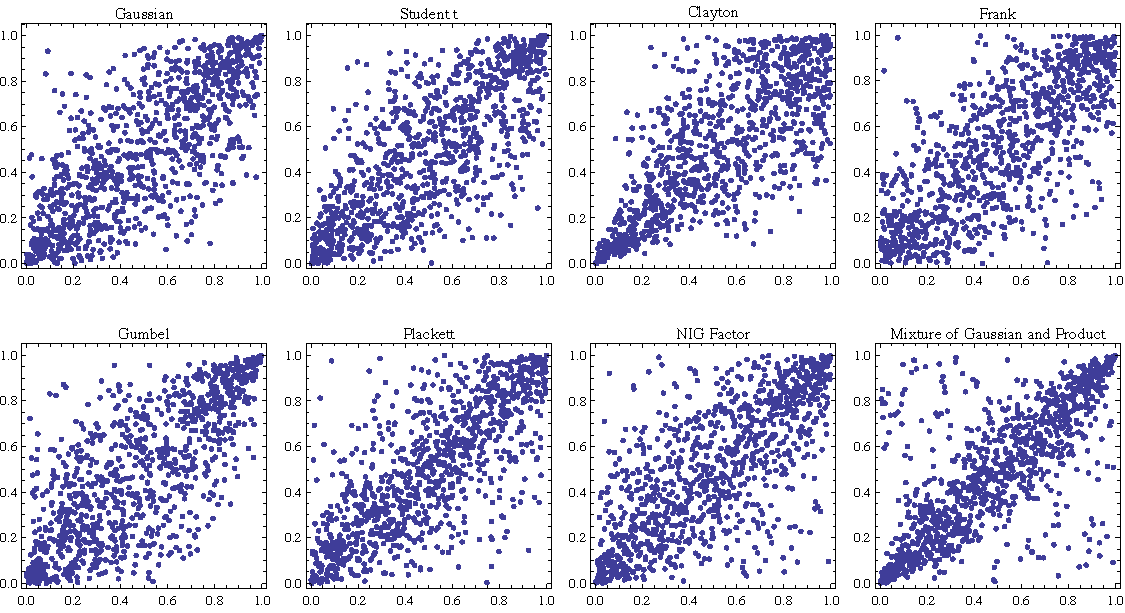
\includegraphics[width=\textwidth]{_pics/copulas_scatterplots.pdf}
  \caption{Scatterplots of samples drawn from various copulae. All
    copulae are calibrated to Spearman's $\rho$ of 0.75 before
    sampling.}\label{fig:copulaeScatterPlot} 
\end{figure}

Kendall's $\tau_K$ and Spearman's $\rho_S$ of the bivariate Gaussian copula are
    \begin{align*}
        \tau_K(\rho) = \frac{2}{\pi}\arcsin\rho
        \end{align*}
    \begin{align*}
        \rho_S(\rho) = \frac{6}{\pi}\arcsin\frac{\rho}{2}.
        \end{align*}

The $t$-copula has the form
\begin{multline*}
        \bm{C}(u,v) = \bm{T}_{2, \rho, \nu}\{T^{(-1)}_\nu(u), T^{(-1)}_\nu(v)\}\\
        = \int_{-\infty}^{T^{(-1)}_\nu(u)}
               \int_{-\infty}^{T^{(-1)}_\nu(v)}
            \frac{\Gamma\left(\frac{\nu+2}{2}\right)}
            {\Gamma\left(\frac{\nu}{2}\right)\pi\nu\sqrt{1-\rho^2}}
             \left(
        1+\frac{s^2-2st\rho+t^2}{\nu}
        \right)^{-\frac{\nu+2}{2}}\, \dd s\, \dd t,
    \end{multline*}
where $\bm{T}_{2, \rho, \nu}$ denotes the 
bivariate $t$ cdf with dependence parameter $\rho$ \natp{\em [Is this
  Spearman's Rho? If so, then say so.]} and degrees of
freedom parameter $\nu$, $\nu>2$,
and where $T^{(-1)}_\nu(\cdot)$ is the quantile function of a standard
$t$ distribution with parameter $\nu$. 

Contrary to the Gaussian copula, the $t$-copula has a non-zero
tail dependence coefficient, which makes it more appropriate for
dependence modelling in finance. The Gaussian copula arises as
$\nu\rightarrow\infty$.

The copula density is
\begin{align*}
    \bm{c}(u,v) &= \frac{\bm{t}_{2, \rho, \nu}\{T^{(-1)}_\nu(u), T^{(-1)}_\nu(v)\}}
    {t_\nu\{T^{(-1)}_\nu(u)\}\cdot t_\nu\{T^{(-1)}_\nu(v)\}},
    \end{align*}
where $\bm{t}_{2,\rho, \nu}$ is the pdf of $\bm{T}_{2, \rho, \nu}$
and $t_\nu$ the density of standard $t$ distribution.

\natp{The $t$-copula and Gaussian copula with parameter $\rho$ have
  equal Kendall's $\tau$, a property shared by all so-called
  elliptical copulas \citep[see][and
references therein]{demarta2005t}. (was: 
Like all the other elliptical copulae, the $t$-copula's Kendall's
$\tau$ is identical to that of the Gaussian copula \citep[see][and
references therein]{demarta2005t}.)}


\subsubsection{Archimedean copulae}\label{sec:archimedean-copula}
The family of Archimedean copulae forms a large class of copulae with
many convenient features.
% Contrary to elliptical copulas, which are derived from
% elliptical distributions.
Archimedean copulas are determined via a simple parametric form of the
dependence structure. A prominent feature is the ability to model
asymmetric dependence structures.  

In general, an Archimedean copula takes the form
\begin{align*}
    \bm{C}(u,v)= \psi^{(-1)}\{\psi(u), \psi(v)\},\quad u,v\in [0,1],
    \end{align*}
where $\psi:[0,1] \rightarrow [0,\infty)$ is a continuous, strictly
decreasing and convex function such that $\psi(1)=0$ \natp{\em [Where
  does $\theta$ come in?]} for any
permissible dependence parameter $\theta$. The function $\psi$ is 
called the generator, with $\psi^{(-1)}$ its inverse.

The {\em Frank copula\/} (B3 in \citet{joe1997multivariate}) takes the form
\begin{align*}
    \bm{C}_{\theta}(u,v) &= \frac{1}{\theta}
    \log \left\{
    1 + \frac{(e^{-\theta u}-1)(e^{-\theta v}-1)}{e^{-\theta}-1}
    \right\}, \quad u,v\in [0,1],
    \end{align*}
    with $\theta \in [0, \infty]$ the dependence parameter. It is a
    radially symmetric copula and cannot produce any tail
    dependence. The following parameters correspond perfect dependence
    and independence: $\bm{C}_{-\infty} = \bm{M}$, $\bm{C}_1 = \bm{\Pi}$,
    and $\bm{C}_\infty = \bm{W}$. The copula density is
    \begin{align*}
      \bm{c}_{\theta}(u,v)
      &= \frac{\theta e^{\theta(u+v)(e^\theta-1)}}
        {\left\{e^\theta-e^{\theta u}-e^{\theta v}+e^{\theta (u+v)}\right\}^2}.
    \end{align*}
    The Frank copula has Kendall's $\tau$ and Spearman's $\rho$ as follow:
\begin{align*}
    \tau_K(\theta) = 1-4\frac{D_1\{-\log(\theta)\}}{\log(\theta)},
    \end{align*}
and
\begin{align*}
    \rho_S(\theta) = 1-12\frac{D_2\{-\log(\theta)\} - D_1\{\log(\theta)\}}{\log(\theta)},
    \end{align*}
where $D_1$ and $D_2$ are the Debye function of order 1 and 2, with
the Debye function defined as $D_n =
\frac{n}{x^n}\int_0^x\frac{t^n}{e^t-1}dt$. \natp{\em [Please find a
  reference for the Debye function. A good candiate is the Handbook by
  Abramowitz Stegun.]}

The {\em Gumbel copula\/} (B6 in \citet{joe1997multivariate}) has
distribution function
\begin{equation*}
  \bm{C}_{\theta}(u,v) = \exp{-\{ (-\log(u))^\theta +(-\log(v))^\theta 
    \}^{\frac{1}{\theta}}},
\end{equation*}
where $\theta \in [1,\infty)$ is the dependence parameter.
It has upper tail dependence with dependence parameter $\lambda^U
= 2-2^{\frac{1}{\theta}}$ and displays no lower tail dependence. 
    
While the Gumbel copula cannot model perfect counter-dependence
\citep{Nelsen2002}, $\bm{C}_{1} = \bm{\Pi}$ models independence, 
and $\lim_{\theta\rightarrow\infty} \bm{C}_\theta = \bm{W}$ models
perfect dependence. The copula density takes the form
%\begin{align}
%        f
%    \end{align}
  \begin{equation*}
    \tau_K(\theta) =\frac{\theta-1}{\theta}. 
   \end{equation*}

The {\em Clayton copula\/} takes the form
\begin{equation*}
  \bm{C}_{\theta}(u,v) = \left\{
    \max(u^{-\theta}+v^{-\theta}-1,0)\right\}^{-\frac{1}{\theta}},
\end{equation*}
where $\theta \in (-\infty, \infty)$ is the dependence parameter.
The Clayton copula, by contrast to Gumbel copula,
generates lower tail dependence with $\lambda^L =
2^{-\frac{1}{\theta}}$, but cannot generate upper tail dependence.
Moreover, $\lim_{\theta\rightarrow -\infty} \bm{C}_\theta = \bm{M}$, $\bm{C}_0 =
\bm{\Pi}$, and $\lim_{\theta\rightarrow\infty} \bm{C}_\theta = \bm{W}$. 
Kendall's $\tau$ of the Clayton copula is given by 
\begin{align*}
    \tau_K(\theta) =\frac{\theta}{\theta+2}.
    \end{align*}

\subsubsection{Mixture Copula}\label{sec:mixture-copula}
The mixture copula is a linear combination of copulae. 
The distribution of a 2-dimensional random variable
$\bm{X}=(X_1,X_2)^\top$ is written as linear combination of $K$
copulae 
\begin{equation*} 
    \bm{C}(u,v)= \sum_{k=1}^K p^{(k)} \cdot \bm{C}^{(k)}\{F^{(-1)}_{X_1}(u),
    F^{(-1)}_{X_2}(v); \bm{\theta^{(k)}}\}, \quad u,v\in [0,1].
  \end{equation*}
  \natp{Here, $\bm{\theta^{(k)}}$ refers to the parameters of the
    $k$-th copula.} Likewise, the copula density is a linear
    combination of copula densities 
\begin{align*}
    \bm{c}(u,v)= \sum_{k=1}^K p^{(k)} \cdot \bm{c}^{(k)}\{F^{(-1)}_{X_1}(u),
    F^{(-1)}_{X_2}(v); \bm{\theta^{(k)}}\}.
    \end{align*}

\natp{\em
  [I think the statement below can go without a formal proof. Here is
  a suggestion].}

   
While Kendall's $\tau$ of the mixture copula is not known in closed form,
Spearman's $\rho$ is easily derived as 
\begin{equation*}
  \rho_S = \sum_{k=1}^K p^{(k)} \cdot \rho_S^{(k)}. 
\end{equation*}

\natp{\em [Old text below.]}

While Kendall's $\tau$ of the mixture copula is not known in closed form,
Spearman's $\rho$ is specified by the following statement. 
\begin{proposition}
  Let $\rho_S^{(k)}$ be Spearman's $\rho$ of the $k$-th component
  Spearman's $\rho$ of the mixture copula is given by 
  \begin{align*}
        \rho_S = \sum_{k=1}^K p^{(k)} \cdot \rho_S^{(k)}.
        \end{align*}
    \end{proposition}

\begin{proof}
  Since Spearman's $\rho$ is defined as \citep{Nelsen1999}
  \begin{equation*}
    \rho_S = 12 \int_{\mathbb{I}^2} \bm{C}(s,t) ds dt - 3,
  \end{equation*}
  Spearman's $\rho$ of the the mixture copula is given by summation
  of the components 
  \begin{align*}
    \rho_S = 12 \int_{\mathbb{I}^2} \sum_{k=1}^K p^{(k)} \cdot
    \bm{C}^{(k)}(s,t) ds dt - 3. 
  \end{align*}
\end{proof}
\natp{\em [Continue here.]}

An example of a mixture copula is the Fr\'echet class of copulae, which
are given by convex combinations of $\bm{W}$, $\bm{\Pi}$, and $\bm{M}$
\citep{Nelsen1999}.  

We use a mixture of Gaussian and independence copulae in our analysis,
i.e., 
\begin{equation*}
  \bm{C}(u,v) = p\, \bm{C}^\text{Gaussian}(u,v) + (1-p)(uv),\quad p\in (0,1),
\end{equation*}
with corresponding density 
\begin{equation*}
  \bm{c}(u,v) = p\, \bm{c}^\text{Gaussian}(u,v) + (1-p).
\end{equation*}

This mixture models the amount of ``random noise'' that appears in the
dependence structure. In the hedging exercise, the
``random noise'' adds an unhedgable component to the two-asset
portfolio, whose weight $(1-p)$ is calibrated from market
data. \natp{\em [Is it clear that the unhedgable part is more than the
  ``random noise''?]}

\subsubsection{NIG factor copula}

The {\em normal inverse Gaussian (NIG)\/} distribution, introduced by
\citep{BarndorffNielsen1997}, has density function
\begin{equation*}
  g(x; \alpha,\beta, \mu, \delta) = \frac{\alpha}{\pi} \e^{\delta
    \sqrt{\alpha^2-\beta^2} -\beta\mu} \frac{1}{q((x-\mu)/\delta)}
  K_1\left[\delta \alpha q\left(\frac{x-\mu}{\delta}\right) \right]
  \e^{\beta x},\quad x>0,
\end{equation*}
where $q(x) = \sqrt{1+x^2}$ and where $K_1$ is the modified Bessel
function of third order and index $1$. The parameters satisfy $0\leq
|\beta|\leq \alpha$, $\mu\in \R$ and $\delta>0$. The parameters have
the following interpretation: $\mu$ and $\delta$ are location and
scale parameters, respectively, $\alpha$ determines the heaviness of
the tails and $\beta$ determines the degree of asymmetry. If
$\beta=0$, then the distribution is symmetric around $\mu$.

The moment-generating function of the NIG distribution is given by
\begin{equation*}
  M(u; \alpha, \beta, \mu, \delta) = \exp\left( \delta
    \left(\sqrt{\alpha^2-\beta^2} - \sqrt{\alpha^2 - (\beta +
        u)^2}\right) + \mu u\right). 
\end{equation*}
As a direct consequence, moments are easily calculated with the
expectation and variance of the NIG distribution being
\begin{align*}
  \mathbb E X &= \mu +
                \frac{\delta \beta}{\sqrt{\alpha^2-\beta^2}}
  \end{align*}
\begin{align} \label{eq:5}
  \text{Var}(X) &= \frac{\alpha^2\delta}{(\alpha^2-\beta^2)^{3/2}}.
\end{align}


The $\text{NIG}(\alpha, \beta, \mu\, \delta)$ distribution belongs to
the class of so-called {\em normal
variance-mean mixture distributions},  (see Section 3.2 of 
\citep{McNeil2005}): $X$ follows an
$\text{NIG}(\alpha,\beta,\mu,\delta)$ distribution if $X$ conditional
on $W$ follows a normal distribution with mean $\mu+\beta W$ and
variance $W$, i.e., 
\begin{equation*}
  X|W\stackrel{\mathcal L}\sim \Ncdf(\mu + \beta W, W),
\end{equation*}
where $W$ follows an {\em inverse Gaussian distribution}, denoted by
$\text{IG}(\delta, \sqrt{\alpha^2-\beta^2})$.

It is easily seen from the moment-generating function that the NIG distribution is preserved under linear combinations, provided
the variables share the parameters $\alpha$ and $\beta$. For this
and other reasons, the NIG distribution is popular in many areas of
financial modelling; for example, it gives rise 
to the normal inverse Gaussian L\'evy process, which may be represented
as a Brownian motion with a time change.

In the setting here, we consider the {\em NIG factor copula}. This is
not directly derived from the multivariate NIG distribution, but
determined through a factor structure instead. The factor structure,
which 
was applied e.g.\ in \citep{Kalemanova2007} for calibrating CDO's,
gives additionaly flexibility as it does not force the components to
have a mixing variable $W$.
The following proposition introduces the NIG factor model and some of
its properties.
\begin{proposition}
  \label{prop:NIG}
  Let $Z\sim \text{NIG}(\alpha, \beta, \mu, \delta)$ and
  $Z_i\sim \text{NIG}(\alpha, \beta, \mu_i, \delta_i)$,
  $i=1,\ldots, n$ be independent NIG-distributed random
  variables. Then:
  \begin{enumerate}
  \item  $X_i = Z + Z_i\sim \text{NIG}(\alpha,\beta,\mu+\mu_i,
  \delta+\delta_i)$,
\item and 
  \begin{align}
    \text{Cov}(X_i,X_j) &= \text{Var(Z)},\nonumber\\
    \text{Corr}(X_i,X_j) &= \frac{\delta}{\sqrt{(\delta+\delta_i)
                           (\delta+\delta_j)}}. \label{eq:6}
  \end{align}
\end{enumerate}
\end{proposition}
\begin{proof}
  \begin{enumerate}
  \item This follows directly from the moment-generating function. 
  \item For the covariance,
    \begin{equation*}
      \text{Cov}(X_i,X_j)
      = \E[(Z+Z_i) (Z+Z_j)] - \E[Z+Z_i] \E[Z+Z_j]
      = \E[Z^2] -(\E Z)^2.
    \end{equation*}
    The correlation is determined directly from \ref{eq:5}.
  \end{enumerate}
\end{proof}

\natp{\em [Please clarify that $\circ$ refers to composition. Clean
  up notation, e.g.\ marginals can be denoted $F_F$ and $F_S$, Use
  just $C$ for the copula. What are $Z_1$ and $Z_2$? I don't find the
  formula in the paper mentioned. Also, where is the formula for
  Kendall's tau taken from?]}
 The NIG factor copula is obtained by transforming the margins to
uniforms (see Sklar's Theorem), giving (e.g.\
\citep{krupskii2013factor}):
\begin{equation*}
  C_{r^S, r^F}(F_{r^S}(r^S), F_{r^F}(r^F)) = \int_\mathbb{R}
  F_{Z_1}(F_{X_1}^{(-1)} \circ F_{r^S}(r^S) -z) \cdot
  F_{Z_2}(F_{X_2}^{(-1)} \circ F_{r^F}(r^F) -z) \cdot
  f_Z(z) dz.
  \end{equation*}
If the margins are continuous, then Spearman's rho of NIG factor
copula is 
\begin{equation*}
  \rho_S = 12 \int \int \int_{\mathbb{R}^3}
  F_{X_1}(x_1) \cdot
  F_{X_2}(x_2) \cdot
  f_{Z_1}(x_1-z) \cdot
  f_{Z_2}(x_2-z) \cdot
  f_Z(z) dx_1 dx_2 dz - \frac{1}{48}.
  \end{equation*}

% \begin{proof}
%   \begin{align}
%   \rho_S(r^S, r^F) &= \rho\{F_{r^S}(r^S), F_{r^F}(r^F)\} \\
%     &= \rho\{F_{X_1}(X_1), F_{X_2}(X_2)\} \\
%     &= 12 \cdot \mathbb{E}\{F_{X_1}(X_1) \cdot F_{X_2}(X_2) \} - \frac{1}{48}\\
%     &= 12 \cdot \int \int_{\mathbb{R}^2} F_{X_1}(X_1) \cdot F_{X_2}(X_2) dF_{X_1,X_2}(x_1,x_2)\\
%     \end{align}
%   Because
%   \begin{align}
%     F_{X_1,X_2}(x_1,x_2) &= \mathbb{P}(X_1 \leq x_1, X_2 \leq x_2)\\
%     &= \mathbb{P}(Z_1 \leq x_1 - Z, Z_2 \leq x_2 - Z) \\
%     &= \int_\mathbb{R}\mathbb{P}(Z_1 \leq x_1 - z) \cdot \mathbb{P}(Z_2 \leq x_2 - z) \cdot f_Z(z) dz,
%     \end{align}
%   so,
%   \begin{align}
%     \rho_S(r^S, r^F) = 12 \cdot \int \int \int_{\mathbb{R}^3} F_{X_1}(x_1) \cdot F_{X_2}(x_2) \cdot f_{Z_1}(x_1 -z) \cdot f_{Z_2}(x_2 -z) \cdot f_{Z}(z) dx_1 dx_2 dz -\frac{1}{48}
%     \end{align}
%   \end{proof}


\subsubsection{Plackett copula}\label{subsec:other-copula}
The Plackett copula has distribution functiono
\begin{align*}
    \bm{C}_{\theta}(u,v) &= \frac{1+(\theta-1)(u+v)}{2(\theta-1)}
                         - \frac{\sqrt{\{
    1+(\theta-1)(u+v)\}^2 - 4uv\theta(\theta-1)}}{2(\theta-1)},
\end{align*}
\natp{where $\theta$...}.
Spearman's Rho is given by 
\begin{align*}
    \rho_S(\theta) = \frac{\theta+1}{\theta-1} - \frac{2\theta \log
  \theta}{(\theta-1)^2}. 
    \end{align*}

The Placket copula possesses a special property, namely
the cross-product ratio is equal to the dependence parameter
\begin{equation} \label{eq:PlackettCrossProduct}
    % &\phantom{=}
    \frac{\p(U \leq u, V \leq v) \cdot \p(U > u, V > v)}
    {\p(U \leq u, V > v) \cdot \p(U > u, V \leq v)}\nonumber
    =
      \frac{\bm{C}_\theta(u,v)\{1-u-v+\bm{C}_\theta(u,v)\}}{\{u-\bm{C}_\theta(u,v)\}\{v-\bm{C}_\theta(u,v)}\nonumber 
    = \theta.
\end{equation}
In words, the dependence parameter is equal to the ratio of the 
number of concordance pairs and the number of discordance pairs of a 
bivariate random variable. 

\natp{\em [Until here.]}

%%% Local Variables:
%%% mode: latex
%%% TeX-master: "SRM"
%%% End:


\section{Estimation}\label{sec:estimation}
%! Author = francis
%! Date = 30.10.20

\subsection{Calibration and selection of copulae}\label{sec:estimation}
We introduce the method to calibrate copulae to our data in this section.
In general, there are two types of calibration procedures to calibrate copulae:
maximum likelihood (MLE) and method of moments (MM).
We decide to deploy the latter since it calibrates according to the moments we desired. \medskip

In the following subsection, we present the configuration of the method of moments procedures we use.
In the subsection after, we argue that MM is more suitable to this work by comparing MM with MLE.

\subsubsection{Method of Moments}
\label{subsec:simulated-method-of-moments}

We trace back the usage of MM to calibrate copulae to \citet{Genest1987, genest1993statistical}.
The moments mainly refer to Kendall's $\tau$ or Spearman's $\rho$.
We extend MM to quantile dependence measures denoted by $\lambda_q$ for quantile level $q$.

Spearman's $\rho$, Kendall's $\tau$, and quantile dependence of the copula $C$ are defined as
\begin{align}
  \rho_S &= 12 \int\int_{I^2} C_{\bm{\theta}}(u,v)\, \dd u\, \dd v-3\label{eq:rho_S}\\
  \tau_K &= 4\E[C_{\bm{\theta}}\{F_X(x), F_Y(y)\}]-1,\\
  \lambda_q &=
  \begin{cases}
    \p(F_X(X)\leq q| F_Y(Y)\leq q) = \displaystyle \frac{C_{\bm{\theta}}(q,q)}{q},
    &\text{ if } q\in (0,0.5],\\
    \p(F_X(X)>q|F_Y(Y)>q) =\displaystyle \frac{1-2q+C_{\bm{\theta}}(q,q)} {1-q},
    &\text{ if } q\in (0.5,1).
  \end{cases}
\end{align}\medskip
The empirical counterparts are
\begin{align*}
  \hat\rho_S &= \frac{12}{n} \sum_{k=1}^n \hat F_X(x_k) \hat F_Y(y_k)
               -3,\\
  \hat\tau_K &= \frac{4}{n}\sum_{k=1}^n \hat{C}\{\hat{F}_X(x_i),\hat{F}_X(y_i)\} -1 ,\\
  \hat\lambda_q &=
                  \begin{cases}
                    \displaystyle\frac{1}{n} \sum_{k=1}^n \frac{\1_{\{\hat
                        F_X(x_k)\leq q, \hat F_Y(y_k)\leq q\}}} {q},
                    &\text { if } q\in (0, 0.5],\\
                    \displaystyle \frac{1}{n} \sum_{k=1}^n
                    \frac{\1_{\{\hat F_X(x_k)>q, \hat F_Y(y_k)>q\}}}
                    {1-q}, &\text { if } q\in (0.5,1),
                  \end{cases}
\end{align*}
where $\displaystyle \hat{F}(x) =
  \frac{1}{n}\sum_{k=1}^n 1_{\{x_i\leq x\}}$ and
$\displaystyle \hat{C}(u,v) = \frac{1}{n}\sum_{k=1}^n 1_{\{u_i\leq u, v_i\leq v\}}$. \medskip

Denote by $\bm{m}(\bm{\theta})$ the $m$-dimensional vector of
dependence measures according the dependence parameters
$\bm{\theta}$,and let $\hat{\bm{m}}$ be the corresponding empirical
counterpart. 
The difference between dependence measures and their counterpart is denoted by
\begin{align*}
    \bm{g}(\bm{\theta}) = \hat{\bm{m}} - \bm{m}(\bm{\theta}).
\end{align*}

The MM estimator is
\begin{align*}
    \hat{\bm{\theta}} = \argmin_{\bm{\theta}\in \bm{\Theta}} \bm{g}(\bm{\theta})^\top
    \hat{\bm{W}}
     \bm{g}(\bm{\theta}),
\end{align*}
where $\hat{W}$ is some positive definite weight matrix.
In this work, we use
$\bm{m}(\bm{\theta}) = (\rho_S, \lambda_{0.05}, \lambda_{0.1}, 
\lambda_{0.9}, \lambda_{0.95})^\top$
for calibration.
$\hat{W}$ is set to identity matrix.

\subsubsection{Comparison of method of moments and maximum likelihood}
\label{subsec:maximum-likelihood-estimation}
By the Hoeffding-Sklar theorem, the joint density of a $d$-dimensional random variable $\bm{X}$ with sample size $n$ can be written as
\begin{equation*}
    \bm{f}_{\bm{X}}(x_1, ..., x_d) = \bm{c}\{F_{X_1}(x_1), ..., F_{X_d}(x_d)\} \prod_{j=1}^d f_{X_i}(x_i).
    \end{equation*}
We follow the treatment of MLE documented in section 10.1 of
\citet{joe1997multivariate}, namely the {\em inference functions for
margins (IFM) method}.
The log-likelihood $\sum^n_{i=1}f_{\bm{X}}(X_{i,1}, ..., X_{i,d})$ can be decomposed into a dependence part and a marginal part,
\begin{align}
    L(\bm{\theta}) &= \sum_{i=1}^n \bm{c}\{F_{X_1}(x_{i,1};\bm{\delta}_1), ..., F_{X_d}(x_{i,d}; \bm{\delta}_d);\bm{\gamma}\}
    + \sum_{i=1}^n \sum_{j=1}^d f_{X_j}(x_{i,j};\bm{\delta}_j)\\
    &= L_C(\bm{\delta}_1, ..., \bm{\delta}_d, \bm{\gamma}) + \sum_{j=1}^d L_j(\bm{\delta}_j)
    \end{align}
where $\bm{\delta}_j$ are the parameters of the $j$-th margin, $\bm{\gamma}$ is the parameter of the parametric copula, and
$\bm{\theta} = (\bm{\delta}_1,..., \bm{\delta}_d, \bm{\gamma})$.
Instead of searching the $\bm{\theta}$ in a high dimensional space, \citet{joe1997multivariate} suggests to
search for $\hat{\bm{\delta}_1},..., \hat{\bm{\delta}_d}$ that maximize $L_1(\bm{\delta}_1), ..., L_d(\bm{\delta}_d)$,
then search for $\hat{\bm{\gamma}}$ that maximize $L_C(\hat{\bm{\delta}_1},..., \hat{\bm{\delta}_d}, \bm{\gamma})$.

%\natp{\em [I suggest to delete the next part, as the regularity
%  conditions are unclear, and it is just a first-order condition,
%  which is a-priori not clear to hold in a two-step procedure.]}
%That is, under regularity conditions, $(\hat{\bm{\delta}_1},..., \hat{\bm{\delta}_d}, \hat{\bm{\gamma}})$ is the solution of
%\begin{align}
%    \left( \frac{\partial L_1}{\partial \bm{\delta}_1}, ..., \frac{\partial L_d}{\partial \bm{\delta}_d},
%    \frac{\partial L_C}{\partial \bm{\gamma}}\right) = \bm{0}.
%    \end{align}

%However, the IFM requires making assumption on the distribution of the
%margins.\natp{\em [delete until here.]}

We follow \citet{genest1995semiparametric} who suggest to replace the estimation of marginals parameters estimation by non-parameteric estimation.
Given non-parametric estimator $\hat{F}_i$ of the margins $F_i$, the estimator of the dependence parameters $\bm{\gamma}$ is
\begin{equation*}
    \hat{\bm{\gamma}} = \argmax_{\bm{\gamma}} \sum_{i=1}^n \bm{c}\{ \hat{F}_{X_1}(x_{i,1}), ..., \hat{F}_{X_d}(x_{i,d});\bm{\gamma}\}.
    \end{equation*}

Both the simulated method of moments and the maximum likelihood estimation are unbiased.
The question though which procedure is more suitable for hedging.

\begin{figure}[h]
%\includegraphics[width=\textwidth]{_pics/t Copula quantile dependence.png}
\includegraphics[width=\textwidth]{_pics/Gumbel Copula quantile dependence.pdf}
\includegraphics[width=\textwidth]{_pics/Clayton Copula quantile dependence.pdf}
  \caption{Quantile dependences of Gumbel, and Clayton Copula. The \textcolor{darkblue}{blue circle dots} are
  the quantile dependence estimates of Bitcoin and CME future, \textcolor{darkblue}{blue dotted lines} are the estimates' 90\% confidence interval.
  \textcolor{orange}{Orange dotted line} is the copula implied quantile dependence by MM estimation.
  \textcolor{lightblue}{Light blue dotted line} is the copula implied quantile dependence by MLE estimation.
%  \href{http://www.quantlet.com/}{\includegraphics[height=\baselineskip]{_pics/qletlogo_tr.png}}
  }
\label{fig:quantile dependence1}
\end{figure}

Figure~\ref{fig:quantile dependence1} shows the empirical quantile dependence of Bitcoin and CME future and the copula implied
quantile dependence of the MLE and MM calibration procedures.
Although the MLE is a better fit to a range of quantile dependence in the middle, it fails to address the situation in the tails.
We find that our data empirically has low quantile dependence in the lower ends ($q<10\%$).
We argue that MM is preferred as it produces a better fit to the dependence
structure in the tail behaviour, contrary to MLE. \medskip

Therefore, we deploy the method of moments throughout the
analysis.
We choose the $5^\text{th}$-, $10^\text{th}$-, $90^\text{th}$-, $95^\text{th}$-quantile, and Spearman's $\rho$ as the moments.


%
%
%\subsection{Two-Stage Estimation}\label{subsec:two-stage-estimation}
%~\cite{joe2005asymptotic} study the efficiency of a two-stage estimation procedure of copula estimation.
%The authors also call this method inference function for margins IFM.
%
%\textbf{Pros}
%\begin{enumerate}
%    \item Almost as efficient as MLE methods but easier to be implemented
%    \item Yields an asymptotically Gaussian, unbiased estimate
%\end{enumerate}
%
%\textbf{Cons}
%\begin{enumerate}
%    \item Subject to specification of marginals \cite{kim2007comparison}
%\end{enumerate}
%
%Our data
%\begin{align}
%    \pmb{y} = \begin{bmatrix}
%                  y_{11} & \cdots & y_{1i}\\
%                  \vdots & \ddots & \vdots \\
%                  y_{n1} & \cdots & y_{ni}
%                  \end{bmatrix}
%    \end{align}
%Let $F$ and $f$ be the joint cdf and joint density of $\pmb{y}$ with parameters $\pmb{\delta}$,
%and let $F_i$ and $f_i$ be the marginal cdf and marginal density for the $i^\text{th}$ random variable with parameters $\pmb{\theta}_i$, we have
%\begin{align}
%    f(\pmb{y}; \pmb{\theta}_1, \pmb{\theta}_2,\dots \pmb{\theta}_i, \pmb{\delta}) =
%    c\{F_1(\pmb{y}_1;\pmb{\theta}_1), F_2(\pmb{y}_2; \pmb{\theta}_2), \dots, F_i(\pmb{y}_1;\pmb{\theta}_i); \pmb{\delta}\}
%    \prod^i_{j=1}f_i(\pmb{y}_j;\pmb{\theta}_j)
%    \end{align}
%
%For a sample of size $n$, the log-likelihood of functions of the $i^\text{th}$ univariate margin is
%\begin{align}
%    L_i(\theta_i) = \sum^n_{m=1} \log f_i(y_{mi}; \theta_i),
%    \end{align}
%
%and the log-likelihood function for the joint distribution is
%\begin{align}
%    L(\delta, \theta_1, \theta_2, \dots, \theta_i) = \sum^n_{m=1}\sum^i_{j=1} \log f(y_{mj}; \delta, \theta_1, \theta_2, ..., \theta_i)
%    \end{align}
%
%In most cases, one does not have closed form estimators and numerical techniques are needed.
%Numerical ML estimation difficulty increase when the total number of parameters increases.
%The two-stage estimation is designed to overcome this problem.
%
%The two-stage procedure is
%\begin{enumerate}
%    \item estimate the univariate parameters from separate univariate likelihoods to get $\tilde{\pmb{\theta}_1}, ..., \tilde{\pmb{\theta}_i}$
%    \item maximize $L(\pmb{\delta}, \tilde{\pmb{\theta}_1}, \dots, \tilde{\pmb{\theta}_i})$ over $\pmb{\delta}$ to get $\tilde{\pmb{\delta}}$
%    \end{enumerate}
%
%Under regularity conditions
%\footnote{Regularity conditions include
%1. $\exists \frac{\partial \log f(x;\theta)}{\partial \theta}, \frac{\partial^2 \log f(x;\theta)}{\partial \theta^2}, \frac{\partial^3 \log f(x;\theta)}{\partial \theta^3}$ for all $x$;
%2. $\exists g(x), h(x) and H(x)$ such that for $\theta$ in a neighborhood $N(\theta_0)$ the relations
%$\left|\frac{\partial f(x;\theta)}{\partial theta}\right| \leq g(x)$,
%$\left|\frac{\partial^2 f(x;\theta)}{\partial \theta^2}\right| \leq h(x)$,
%$\left|\frac{\partial^3 f(x;\theta)}{\partial \theta^3}\right| \leq H(x)$ hold for all $x$, and
%$\int g(x) dx < \infty$, $\int h(x) dx < \infty$, $\mathbb{E}_\theta \{H(X)\} < \infty$ for $\theta \in N(\theta_0)$;
%3. For each $\theta \in \Theta$, $0< \mathbb{E}_\theta \left\{
%\left(
%\frac{\partial \log f(X;\theta)}{\partial \theta}
%\right)^2
%\right\}$. For detail see section 4.2.2 of~\cite{serfling2009approximation}}
%, $(\pmb{\tilde{\theta}}_1,\dots \pmb{\tilde{\theta}}_i, \pmb{\tilde{\delta}})$ is the solution of
%\begin{align}
%    (\partial L_1 / \partial \pmb{\theta}^\intercal_1,
%    \dots, \partial L_i / \partial \pmb{\theta}^\intercal_i, \partial L / \partial \pmb{\pmb{\delta}}^\intercal_1) = \pmb{0}
%    \end{align}
%
%For comparison, if we optimize $L$ directly without the two-stage procedure (i.e.~MLE), we solve for
%\begin{align}
%    (\partial L / \partial \pmb{\theta}^\intercal_1,
%    \dots, \partial L / \partial \pmb{\theta}^\intercal_i, \partial L / \partial \pmb{\pmb{\delta}}^\intercal_1) = \pmb{0}
%    \end{align}
%
%We denote the two solutions as
%$\tilde{\pmb{\eta}} = (\pmb{\tilde{\theta}}_1,\dots \pmb{\tilde{\theta}}_i, \pmb{\tilde{\delta}})$ for two-stage procedure;
%$\hat{\pmb{\eta}} =(\pmb{\hat{\theta}}_1,\dots \pmb{\hat{\theta}}_i, \pmb{\hat{\delta}})$ for MLE procedure.
%and compare the asymptotic relative efficiency of $\tilde{\pmb{\eta}}$ and $\hat{\pmb{\eta}}$.
%
%Asymptotics: yet to be done.\\
%~\cite{kim2007comparison} show the estimation of $\pmb{\theta}$ may be seriously affected.
%They compare the two-stage approach and Canonical Maximum Likelihood Method by simulation and
%conclude that Canonical Maximum Likelihood is prefered from a computational statistics and data analysis point of view.
%
%\subsection{Canonical Maximum Likelihood Method}\label{subsec:canonical-maximum-likelihood-method}
%This approach was studied by~\cite{genest1995semiparametric} and~\cite{shih1995inferences}.
%One estimates the margins using empirical CDF
%\begin{align}F_X(x)=\frac{1}{n+1}\sum_{i=1}^n 1(X_i \leq x)\end{align},
%
%we maximize the log-likelihood
%\begin{align}
%    L(\delta) = \sum_{i=1}^n \log [c_\delta \{F_X(X_i), F_Y(Y_i)\}]
%    \end{align}
%
%This procedure does not require specification of marginals.
%
%
%
%
%
%%also by Wang and Ding, 2000; Tsukahara, 2005
%%This is also known as pseudo maximum likelihood (PML) and as canonical maximum likelihood (see Cherubini et al., 2004)
%%
%%Genest and Werker (2002) obtained conditions under which the PMLE is asymptotically efficient.
%%
%%


%%% Local Variables:
%%% mode: latex
%%% TeX-master: "SRM"
%%% End:


\section{Data and margins}\label{sec:data-and-margins}
TODO:
\begin{itemize}
    \item Data description
    \item KDE and bandwidth selection
    \item plots
    \item Data preprocessing, the 300-30 train-test split, moving window estimation etc
\end{itemize}

\section{Results}\label{sec:results}
In this section, we provide the result of hedging BTC with BTC future using different copulae and risk measures.
The results is drawn using the data from 29/12/2017 to 27/05/2021 (15/12/2017 is the first trading day of the CME BTC future).
BTC price is obtained from Tiingo, a data provider who aggregate BTC prices of major exhanges in the market;
BTC future price is quoted by CME and retrieved as daily closing price from Bloomberg Terminal.
\medskip

Before estimating the optimal hedge ratio, we pre-process the data as follow.
First, we inner joint the daily BTC price and BTC future by date,
i.e. match the prices with date and discard the unmatched.
Then, we compute the log returns by $r_t = \log \frac{P_t}{P_{t-1}}$ where $P_t$ is the price of an asset at time time $t$.
We use this log return to estimate h and evaluate $h$’s performances. \medskip

After preprocessing the data, we search $h^*$ for each copula-risk-measure pairs as follow.
First, we compute the the marginal distributions by empirical CDF (ECDF) for each training dataset.
Each training dataset consists of 300 returns.
The ECDF is $\hat F(x) = \frac{1}{300}\sum_{n=1}^{300} r \cdot 1(r \leq x)$.
Then, we calibrate copulae with the marginal ECDF by the method of moments mentioned above.
Next, we draw samples from copula and, with the samples, numerically search for the $h^*$ which minimise the risk measure.
We draw one million samples from copula for each search.
The $h^*$ is then applied to the out-of-sample data.
The out-of-sample is the data of the consecutive 5 trading day to the training data (window size of $5$).
The $h^*$ is indexed with the first date of the out-of-sample data.
We then shift the data with $5$ trading days and repeat the procedure (step size of $5$). \medskip

\subsection{Profit and Loss}\label{subsec:empirical-results}

%Figure~\ref{fig:Gumbel} shows the result of the Gumbel-Variance.
%One can see that the fluctuation of the hedged log returns is smaller then that of the BTC and BTC future.
%The extreme negative returns (red dots) of BTC is well managed by the hedge. \medskip
%%One can see all the combinations of copula and risk reduction objective generate a large fluctuation of returns in
%%25/09/2019 and 26/09/2019.
%%This large fluctuation is due to dependence break.

Figure~\ref{fig:Gumbel} shows the time series of out-of-sample $r^h$ using the NIG factor copula with the
objective of reducing variance.
The red dots are the 30 most extreme negative returns in Bitcoin.
In the figure, we can see the downside risk of Bitcoin is well managed by the hedging procedure with NIG factor copula.
Most of the extreme losses of Bitcoin are greatly reduced by introducing the CME future in the hedged portfolio.
Two exceptions are found in 25/09/2019 and 26/09/2019, where the CME future failed to follow the large drop in Bitcoin.
%The reason of drop is unknown, but sudden drop in price is common in the cryptocurrency market.
One of the possible reason is that traders was performing rollover activities on 25-26/09/2019, which
27/09/2019 is the expiry day of the September future.
Another reason for the NIG factor copula fail of capturing the loss is dependence break.
The Kendall's tau in the training data is 0.2 higher than that of the testing data.
Other copulae suffer from the break as well. \medskip
%
\begin{figure}[th]
   \centering
   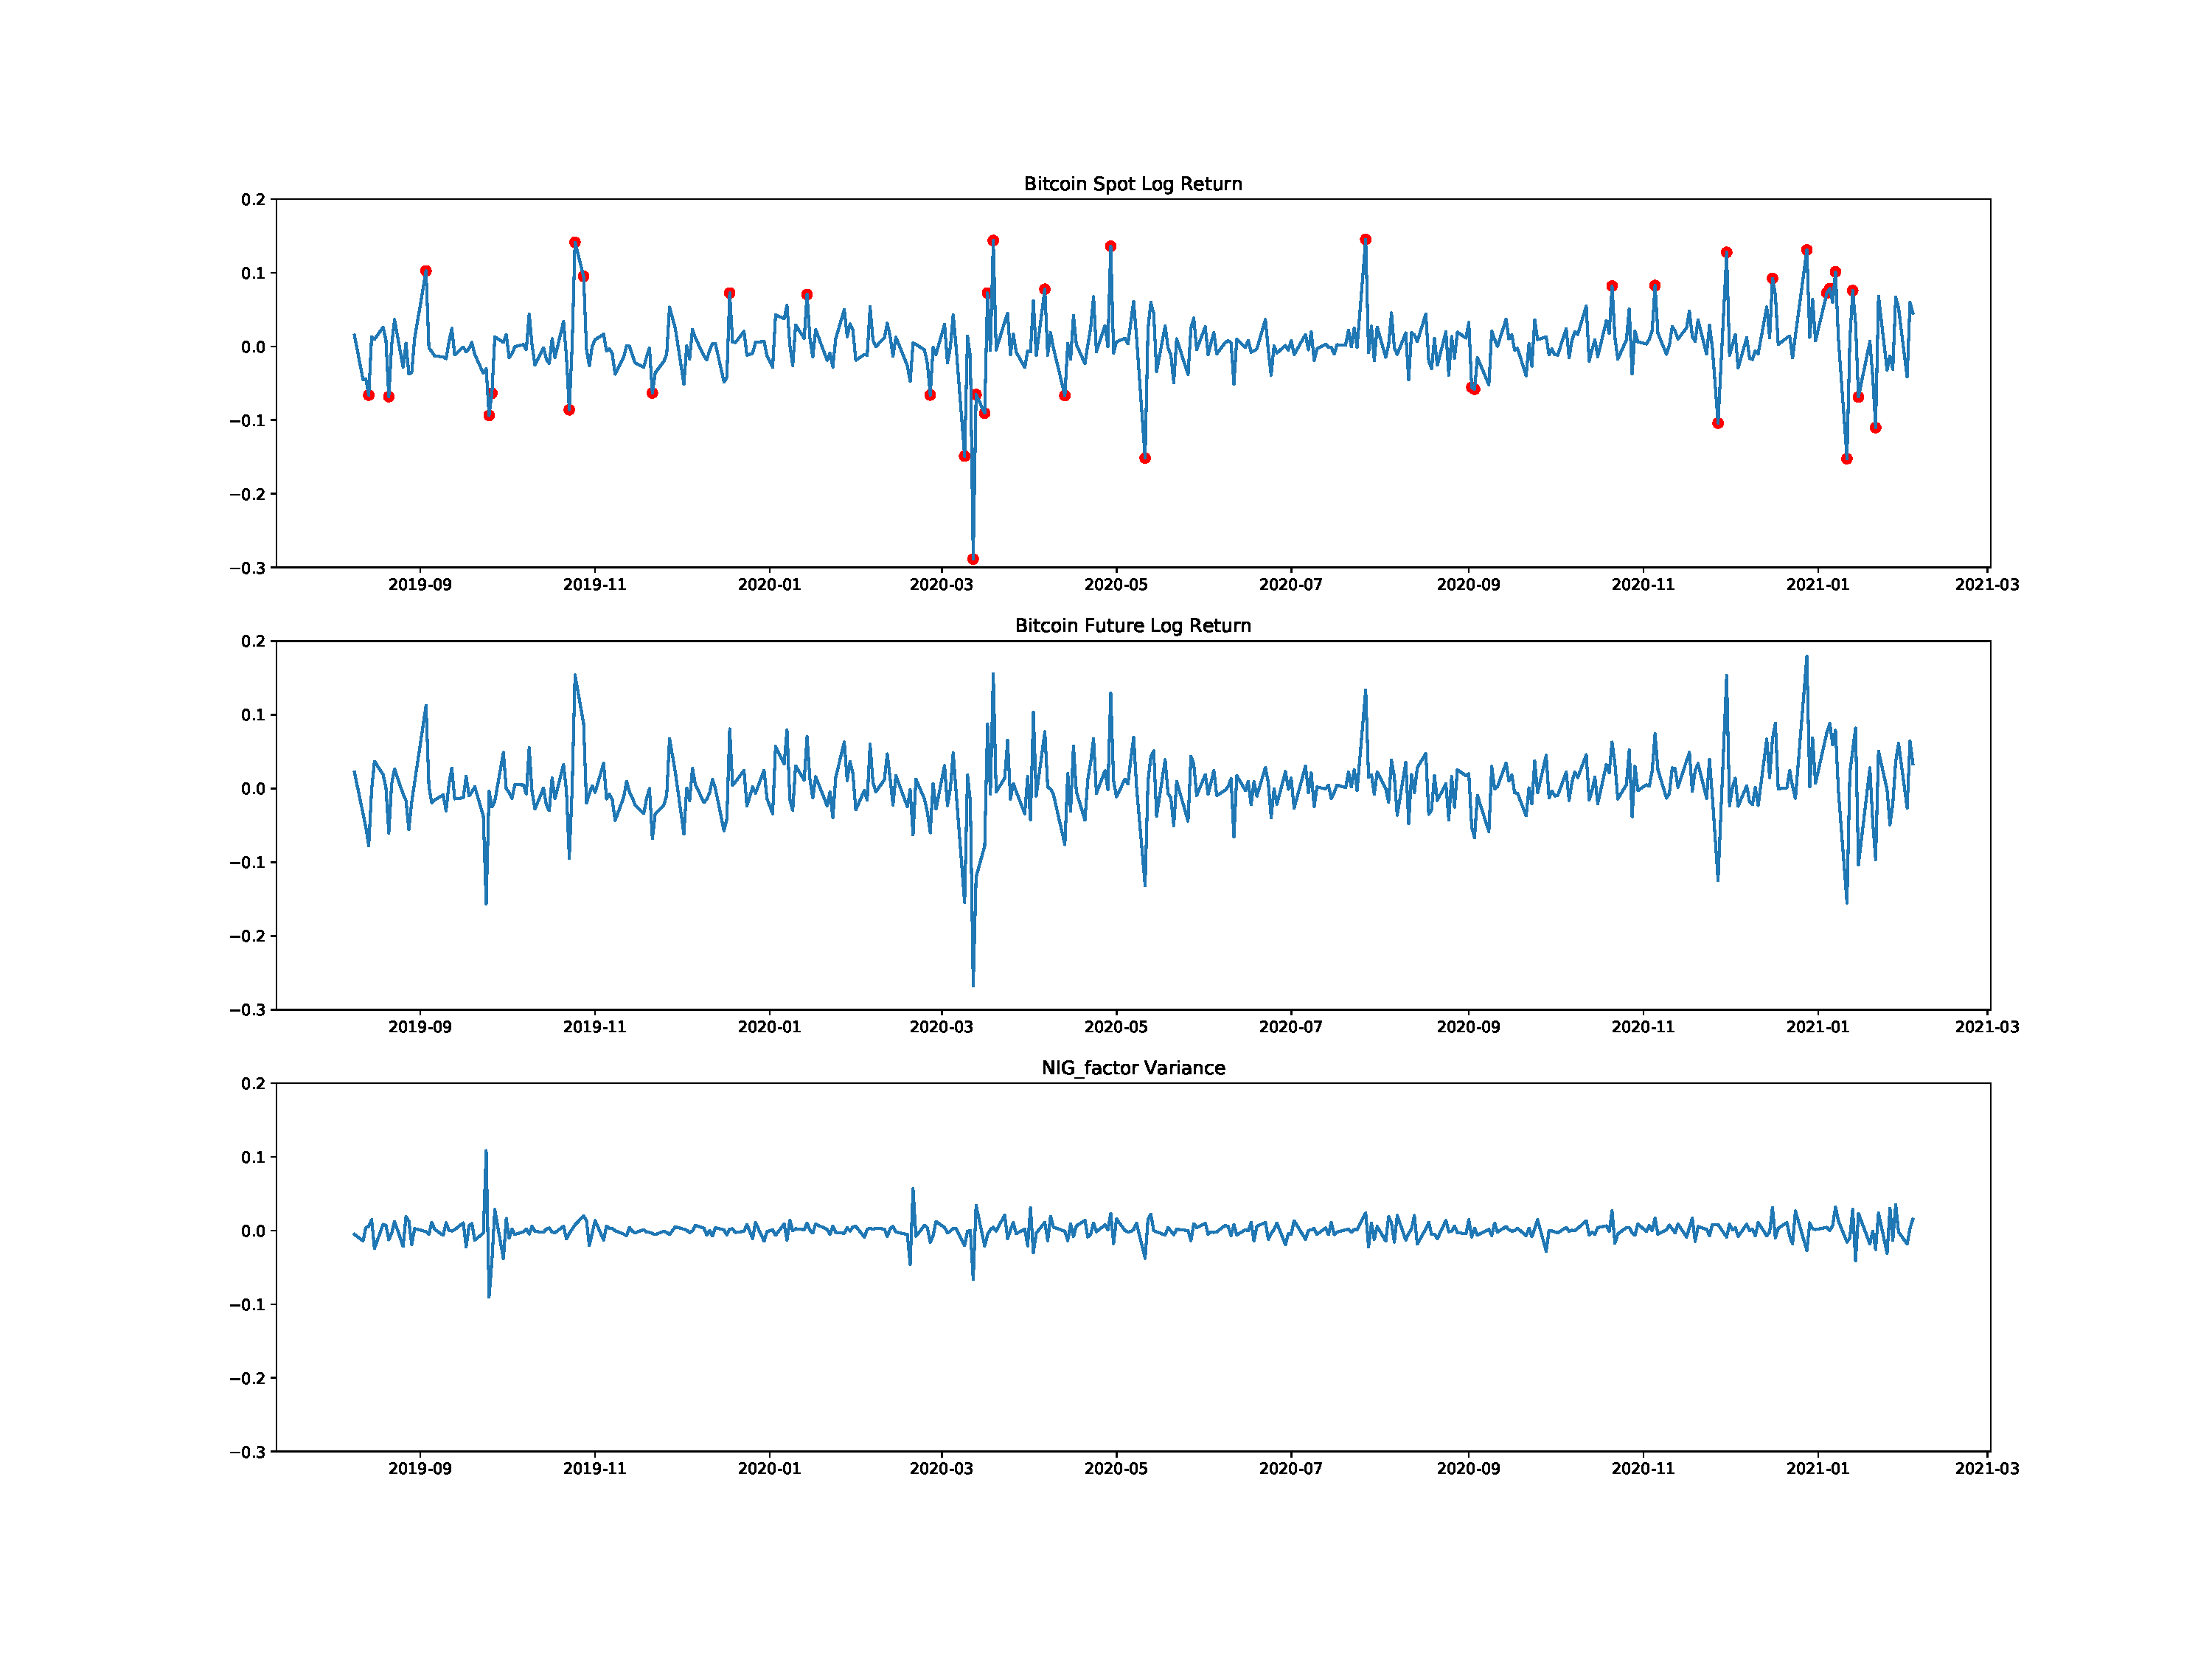
\includegraphics[width=\textwidth]{_pics/OOSreturns_compare.pdf}
   \caption{First Panel: Out of Sample Log-return of Bitcoin; Second Panel: Out of Sample Log-return of Future;
   Third Panel: Out of Sample Log-return of Hedged Portfolio by NIG factor copula with the aim of variance reduction.
   The red dots indicate the lowest 10\% return of Bitcoin, i.e. large negative moments of price.
%   Forth Panel: Out of Sample Log-return of Hedged Portfolio by $h=1$ (naive hedge).
%   Lower Panel: Out of Sample Hedged Portfolio log-returns.
%   The $h^*$ is obtained from Gumbel copula aiming at reducing variance.
%   The red dots indicate the 30 most extreme negative returns in Bitcoin.
   \href{http://www.quantlet.com/}{\includegraphics[width=20pt]{_pics/qletlogo_tr.png}}}
   \label{fig:Gumbel}
\end{figure}

Results of the other pairs are very similar, they are documented in
figure~\ref{fig:OOSRH} in the appendix.
The figure tabulates the time series of out-of-sample returns of hedged portfolio under various copulas and risk reduction objectives.\medskip

\subsection{Evaluation}\label{subsec:evaluation}
In addition to the PnL generated by different copula-risk-measure pairs,
we evaluate their performance by hedging effectiveness (HE), root mean squared error (RMSE), and downside semivariance (SV).
The purpose of evaluating performances of copula-risk-measure pairs beyond PnL is to assist the judgement of which pairs can estimate the optimal hedge ratio which
are suitable to hedge BTC with its future.
, in particular, HE measures the reduction of risk, the RMSE and SV relate investors' preference
(via utility function) while judging which random outcomes are better than the other.

%We illustrate the results in three directions, hedging effectiveness,
%ability of hedging extreme negative events in $r^S$, and the stability of $h^*$.

%\begin{itemize}
%   \item  Hedging Effectiveness
%   \begin{itemize}
%     \item Kick out Frank for its ineffectiveness; Alternative to a one-parameter symmetric Archimedean copula is Plackett;
%       \natp{\em [The issue with the Frank copula is that is has no
%         tails. A scatterplot looks like a strip, there is no
%         concentration in the tails. For CDO pricing (and this is what
%         I remember from my PhD studies) this poses problems as you
%         move from senior to junior tranches. Here, I suppose it just
%         does not capture the empirical behaviour of the data.
%         ]}
%     \item Differences among combinations of copula and risk reduction objective are small;
%     \item None of the combination can escape from the structural break point (dependence of training is stronger then that of testing). (The bump in 25-26th Sept 2019)
%     \item The best performing RRO of a particular risk measure in out-of-sample $r^h$ is not necessarily same, e.g.
%      VaR 95\% as RRO (with Gumbel copula) can generate the lowest out-of-sample ES 99\%.
%   \end{itemize}
%   \item Ability to hedge extreme events in $r^S$
%   \begin{itemize}
%     \item The extreme events in $r^S$ are well managed by the hedge.
%     The magnitudes of loss in $r^h$ is much smaller than that of $r^h$. (Visually seen from the time series of $r^h$)
%     \item None of the combination can escape from the structural break point (dependence of training is stronger then that of testing)
%   \end{itemize}
%   \item Stability of $h^\ast$
%   \begin{itemize}
%     \item Gumbel gives high $h$ all the time; the extreme events are "hedged" ex-ante.
%     \item ES 99\% and VaR 99\% as risk reduction objective are too sensitive to extremes in training data;
%     Large changes in $h$ are suggested in response to extremes training data, while the testing data are less extreme;
%     \item ERM can be seen as a smoothed risk measure focusing in the lower tail of $r^h$; Less sensitive to rare events; Suggested.
%   \end{itemize}
%\item \end{itemize}

\subsubsection{Hedging Effectiveness}\label{subsubsec:hedging-effectiveness}
The hedging effectiveness (HE) measures the reduction of portfolio risk.
This notion of evaluating of hedging performance was proposed by \citet{ederington1979hedging} in the context of hedging the newly introduced
organized futures market.\medskip

HE is defined as
\begin{align}
  1- \frac{\rho(r^h)}{\rho(r^S)},
  \end{align}
where $\rho$ is a risk measure.

We measure the HE of copula-risk-measure pairs according to the risk measure, for example we measure the
HE of Gaussian-ES99\% pair by
\begin{align}
  1- \frac{\text{ES}_{99\%}(r^h)}{\text{ES}_{99\%}(r^S)},
  \end{align}
where $r^h$ is out-of-sample return generated by Gaussian-ES99\%, and $r^S$ is the out-of-sample log return of BTC. \medskip

\begin{figure}[H]
   \centering
   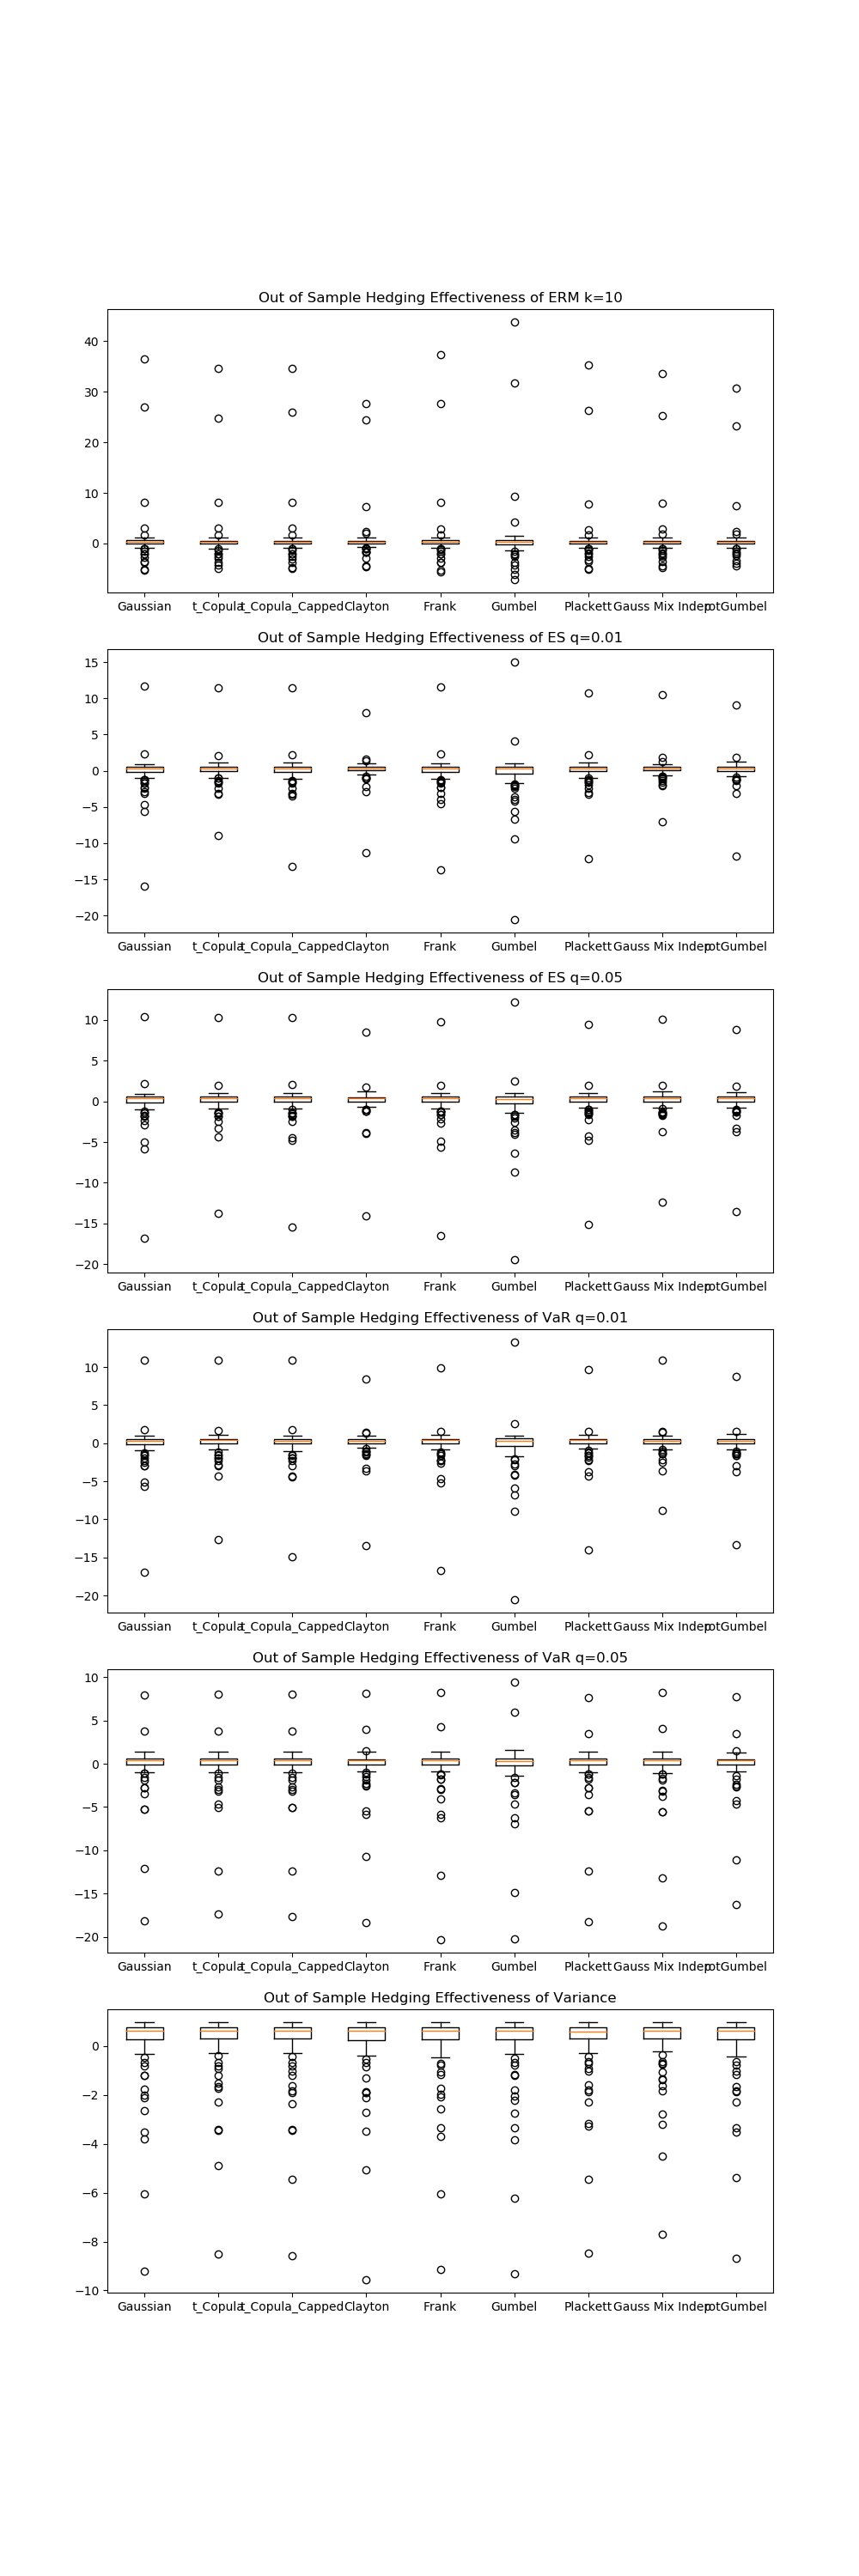
\includegraphics[height=24cm]{_pics/Out of Sample Hedging Effectiveness.png}
   \caption{Out of Sample Hedging Effectiveness Box-plot.
   The HEs are obtained from a set of out-of-sample data,
   each set consists 30 days log returns of Bitcoin and CME future.
   \href{http://www.quantlet.com/}{\includegraphics[width=20pt]{_pics/qletlogo_tr.png}}}
   \label{fig:OOSHE}
\end{figure}

The box-plots in figure \ref{fig:OOSHE} show the out-of-sample hedging effectiveness of different copulas under various risk
reduction objectives across testing datasets.
Observe that most of the copulae perform well.
The average HE of copulas and risk reduction objectives is higher than 60\% except for Frank-copula.
However, the HEs vary a lot in different testing data.
In some instances, the HE can be as low as 10\%.
This reflects the highly violate nature of cryptocurrencies:
the optimal hedge ratio in the training data deviates from that of testing data.
There is a large literature about structural break points and time changing dependence, to name a few
\citet{hafner2012dynamic}, \citet{patton2006modelling}, \citet{creal2008general},
\citet{engle2002dynamic}, \citet{giacomini2009inhomogeneous}, and also
\citet{manner2012survey}.\medskip

\subsubsection{Root Mean Squared Error and Semivariance}
Root mean squared error (RMSE) and semivariance (SV) are special cases of the Bernel Stone's generalized risk measure \citep{stone1973general}.
The purpose of applying a generalized risk measure is to measure the hedge performance of copula-risk-measure pairs in a common ground. \medskip

The Bernel Stone's generalized risk measure is
\begin{align*}
    \rho(F) = \int_{-\infty}^{\gamma(F)} \left|x-\eta(F)\right|^\alpha dF(x),
    \end{align*}
where $F$ is the distribution of the uncertain return, parameters $\alpha$ is chosen to represent preferences of investors,
$\eta(F)$ is a reference level of wealth from which deviations are measured, and $\gamma(F)$ is a range parameter that specifies the range of deviations to be included.\medskip

\citet{fishburn1977mean} justifies the usage of generalized risk measure (with his $\alpha$-$t$ model) by connecting the measure with Von Neumann-Morgenstern utility theorem, see also \citet{bawa1975optimal, bawa1978safety}
and \citet{morgenstern1953theory}.
We argue that evaluation of hedging performance of a crypto portfolio does not differ from this classical framework:
crypto investors maximise expected utility with given utility functions.
Vast body of recent literature remain in this classical framework, to name a few, \citet{sebastiao2020bitcoin, deng2020minimum, cui2020composite, oglend2020futures}. \medskip
See also \citet{chen2003futures} for a review of hedging performance evaluation.

%Hedging futures performance with denoising and noise-assisted strategies
%Minimum-variance hedging of Bitcoin inverse futures

For root mean squared error, we choose $\gamma(F)=\infty$ and $\eta(F)=0$, i.e. we consider a full range, from $-\infty$ to $\infty$, of deviations to our target
of zero PnL.
For semivariance (SV), we choose $\gamma(F)=0$ and $\eta(F)=\operatorname{\mathbf{E}}(r|r \leq 0)$.
The setting of semivariance represents our focus on the downside risk.
Sometimes, SV is called lower partial moment. \medskip

Therefore, for each pair of copula-risk-measure, we calculate
\begin{align*}
    \text{RMSE} = \operatorname{\mathsf{E}}\{(r-0)^2\}^{1/2},
    \end{align*}
and
\begin{align*}
    \text{SV} = \operatorname{\mathsf{E}}\left[\{r - \operatorname{\mathsf{E}}(r|r \leq 0)\}^2 | r \leq 0 \right].
\end{align*}

\begin{figure}%
    \centering
    \subfloat{{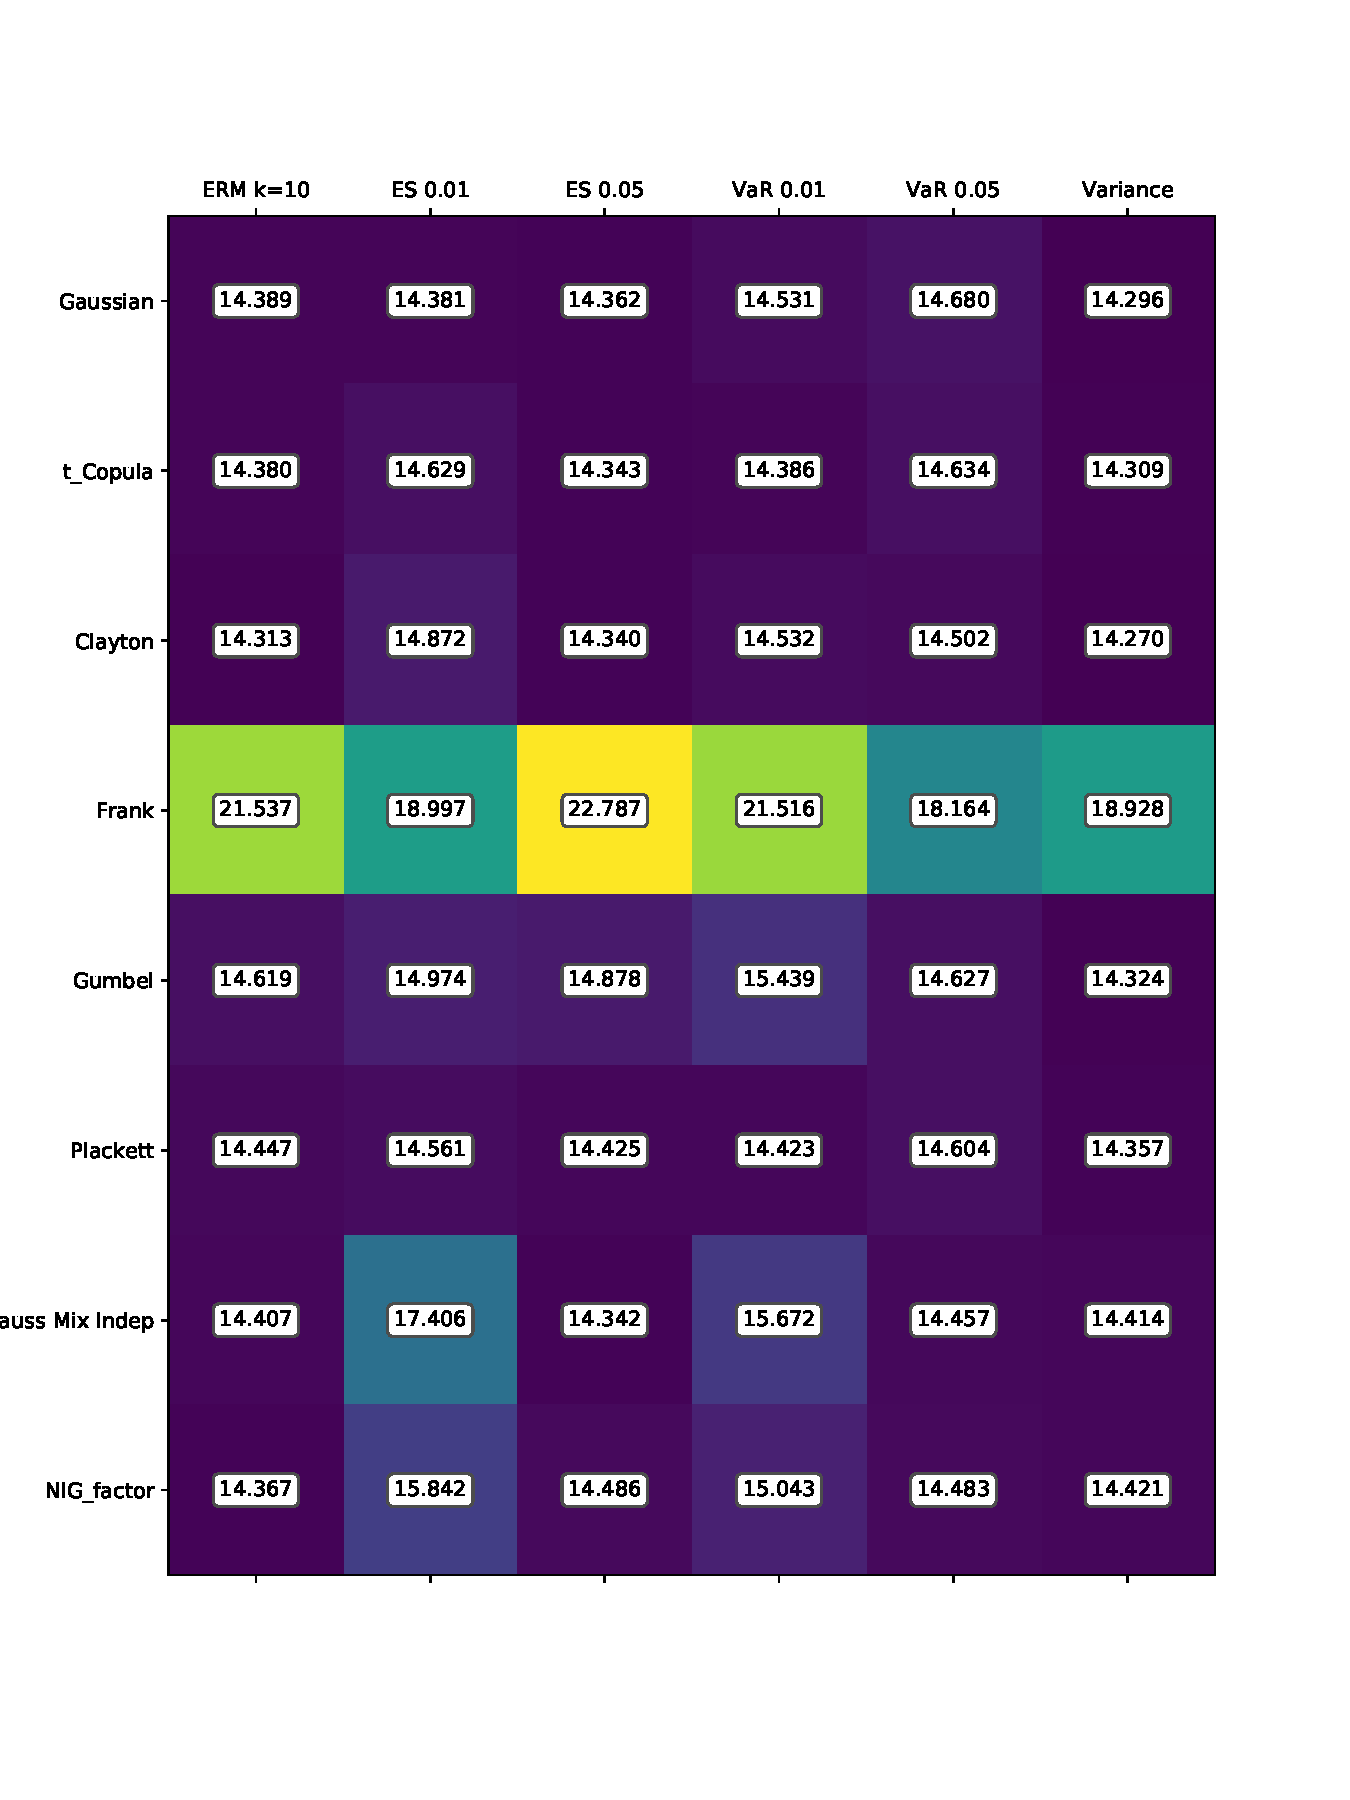
\includegraphics[width=.45\textwidth]{_pics/rmse_static.pdf} }}%
    \qquad
    \subfloat{{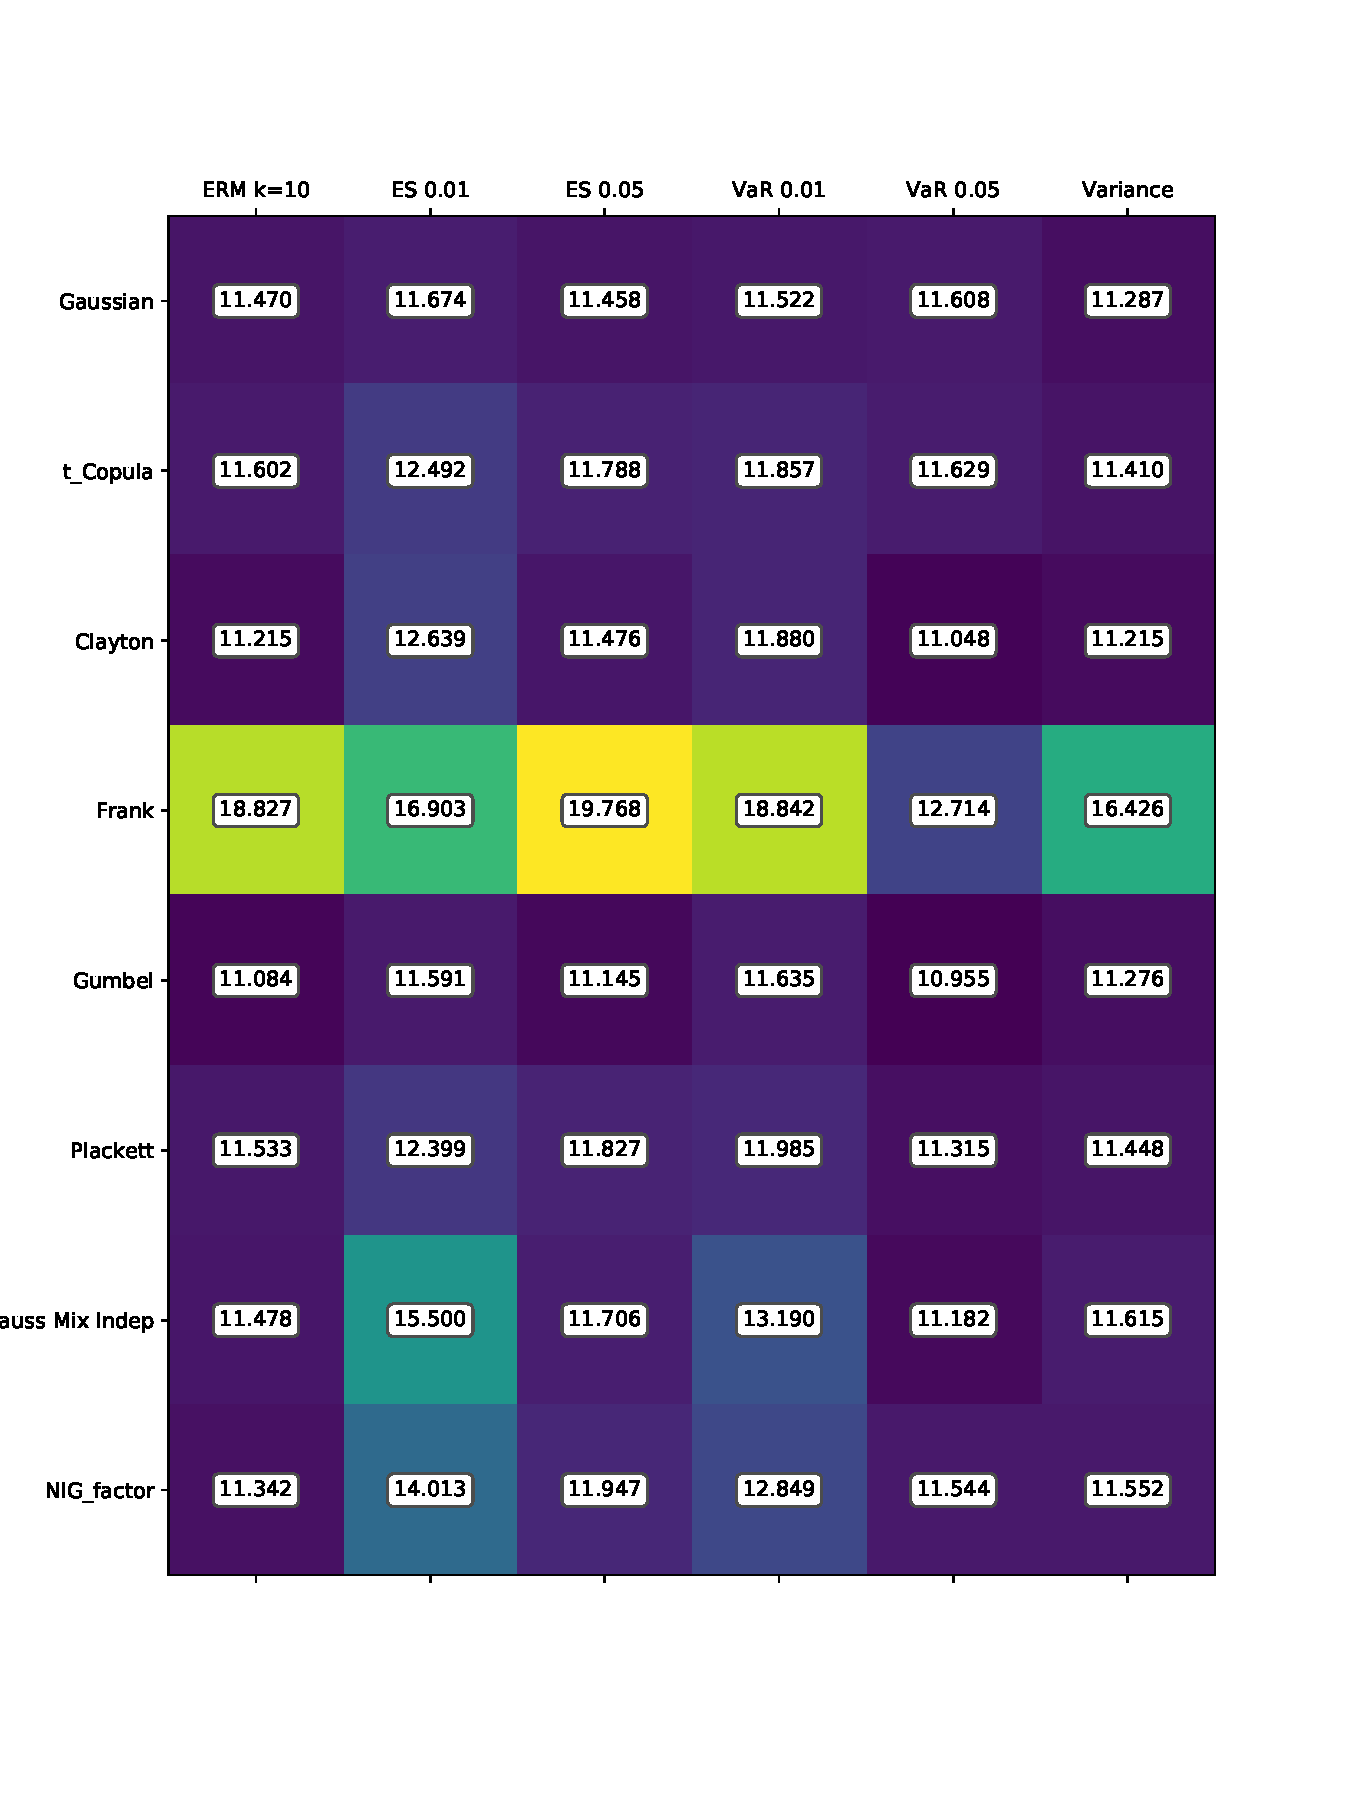
\includegraphics[width=.45\textwidth]{_pics/semivariance_static.pdf} }}%
    \caption{Left panel: RMSE$\cdot 1000$ of different copula-risk-measure pairs; Right panel: $\text{SV}^{0.5}\cdot 1000$ of
    different copula-risk-measure pairs. Frank copula is inferior to other copulae in terms of RMSE and SV.
    ES99\% and VaR99\% have slightly higher RMSE and SV.
%   Forth Panel: Out of Sample Log-return of Hedged Portfolio by $h=1$ (naive hedge).
%   Lower Panel: Out of Sample Hedged Portfolio log-returns.
%   The $h^*$ is obtained from Gumbel copula aiming at reducing variance.
%   The red dots indicate the 30 most extreme negative returns in Bitcoin.
   \href{http://www.quantlet.com/}{\includegraphics[width=20pt]{_pics/qletlogo_tr.png}}}%
    \label{fig:rmse_sv}%
\end{figure}

The result is shown in figure~\ref{fig:rmse_sv}.
The RMSE of the copula-risk-measure pairs is ranging from 0.014 to 0.023.
The smallest RMSE is generated by the pair Clayton-Variance, while a number of other pairs generate very similar results.
In particular, RMSEs of variance are relatively low while comparing with other risk measures across different copulae.
This is a natural result.
The Frank copula's RMSEs are high no matter the risk measures.
This suggests Frank should not be used to model the dependency structure of BTC and BTC future.\medskip

%RMSEs of VaR 99\% and ES 99\% across different copulae are also inferior to that of other risk measures.
%We will discuss this result in the robustness part. \medskip

The SV of the copula-risk-measure pairs is ranging from 0.011 to 0.020.
The best performing pair in terms of SV is Gumbel-VaR95\%.
Gumbel copula also has the lowest or second lowest SV while comparing with other copulae across different risk measures.
It is not surprising that Gumbel copula is superior than the other copula:
the dependency of positive jumps in BTC and BTC future is captured by Gumbel copula, while in our dataset,
positive jumps in BTC is frequent.
Furthermore, VaR95\% has the lowest or second lowest SV while comparing with other risk measure across different copulae.
Similar to the result in RMSE, various the copula-risk-measure pairs' SV performance are similar, except for Frank copula, VaR99\%, and ES99\%.

%\begin{figure}[t]
%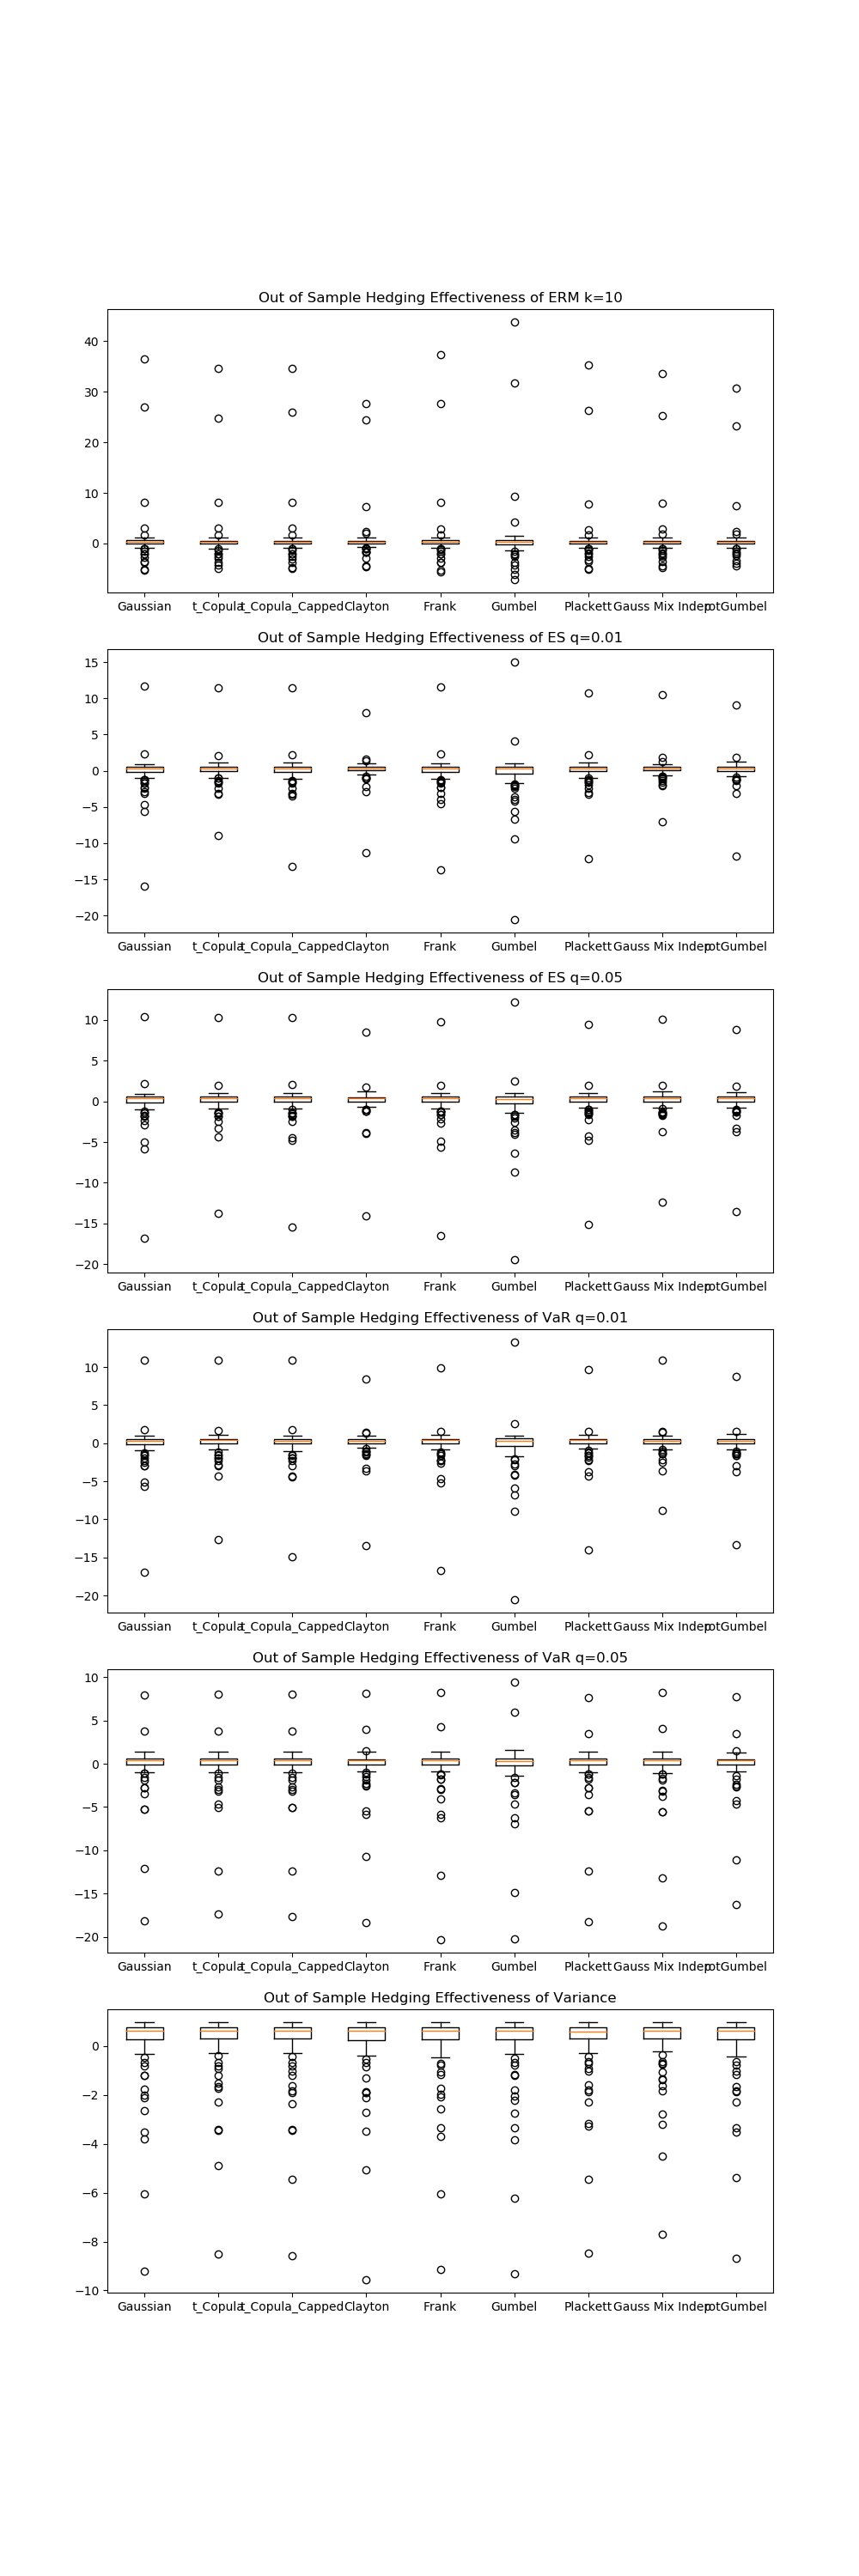
\includegraphics[width=\textwidth, height=\textheight]{_pics/Out of Sample Hedging Effectiveness.png}
%  \caption{}
%\label{out of Sample Hedging Effectieness}
%\end{figure}

%\subsubsection{Semivariance}
%Semivariance is a measurement of data to estimate the potential downside risk of an investment portfolio.
%It is the dispersion of all observations that is smaller than the mean or a certain threshold.
%Semivariance is discussed by many, to name a few,
%Markowitz (1959), Mao (1970a, 1970b),
%Mao (1970a), Hogan and Warren (1972, 1974).
%provide the theoretical justifications for semivariance.
%\subsection{Stability of $h^*$}

\section{Conclusion and Discussion}
In this paper, we model the dependency between Bitcoin (BTC) and its future via various copulae and search for
the optimal hedge ratios $h^*$ minimising different risk measures.
We conclude that various copulae, except the Frank copula, are appropriate to model the dependency structure between Bitcoin and its future when we want to minimise risk.
In addition, one should avoid using Value-at-Risk 99\% or Expected Shortfall 99\% as loss function while searching for the optimal $h^*$.
Other risk measures are ready to be deployed according one's objective.
The hedging effectiveness (HE) of various copula-risk-measure pairs are close to 65\%, i.e.
the risk of a portfolio of Bitcoin, measured by a particular risk measure, is reduced
by 65\% by including an optimal amount $h^*$ of Bitcoin future.
Again, the Frank copula is inferior to other copulae in terms of HE.
We also compare the root mean squared error (RMSE) and semivariance (SV).
Unsurprisingly, we can rule out the Frank copula, Value-at-Risk 99\% and Expected Shortfall 99\%
for hedging Bitcoin and its future.

\subsection{About Frank Copula}\label{subsec:Frank}
Frank-copula, in general, is not a good choice to model financial data.
We can see from figure~\ref{fig:Frank} that the Frank copula is not fitting the Bitcoin and its future visually, no matter
which optimization procedure is being deployed.
The samples of Frank diffuse like a strip with parallel edge when the parameter $\theta$ decrease (samples are being less dependent).
This makes Frank copula not a a good fit to the data.

\begin{figure}[th]
   \centering
   \includegraphics[width=\textwidth]{_pics/Frank.pdf}
   \caption{Comparison of Frank Copula Samples and Pseudo Observations of Bitcoin and CME Future Returns.
   \href{http://www.quantlet.com/}{\includegraphics[width=20pt]{_pics/qletlogo_tr.png}}}
   \label{fig:Frank}
\end{figure} \medskip

Aside from the Frank-copula, the HEs of various combination of copula and risk reduction objective are very similar.
This is an expected result as the portfolio consists only two assets.

\subsection{Robustness}\label{subsec:robustness}
The study of robustness concerns the stability of statistical estimation with respect to violation in assumptions.
In our context, the robustness is with respect to outliers (or jumps).
It is natural to do we want the optimal hedge ratio react to extreme market changes?
In practice, outliers of returns can come from anywhere, for example, a tweet from Elon Musk, a sudden large order from
institutional investor, or an incident of system failure in cryptocurrency exchanges.
Rapid and drastic changes in portfolio weight causes problem of slippage and transaction cost.
Investors should be aware of the cost brought by the sensitivity of the optimal hedge ratio procedure.
\medskip

The discussion of sensitivity or robustness dates back to \citet{huber1981robust}'s work on robust statistics.
\citet{hampel2011robust} suggest an infinitesimal approach to investigate sensitivity of statistical procedures.
There are three central concepts in this approach, qualitative robustness, influence function, and break-down point.
They are loosely related to the concept of continuity, first derivative of functional, and the distance of a functional to its nearest pole (singularity).
While the first concept is a qualitative feature of a functional, the second the third concepts are practical tools to measure sensitivity quantitatively.
We deploy a finite sample version of the second and third concepts.
Details of robustness of risk measures can be found in \citet{cont2010robustness}. \medskip

%\francis{\em [FL: Need to rewrite the following to show the IF of hedge performance instead of h. But Please have a look of the methodology first.]}
%With a probability space $(\Omega, \F, \p)$,
%we denote $M: \Omega \mapsto \mathscr{C}, M \in \{\text{MLE}, \text{MM}, \text{Empirical}\}$ be estimators of interest for distribution of returns,
%$$\mathscr{C} = \{\text{Gaussian-Copula}, ..., \text{Plackett-Copula}, \text{Empirical-Copula}\} \in \p$$ be a set of bivariate distributions of interest,
%$\rho_{h}: \mathscr{C} \mapsto \mathbb{R}$ be a risk measure on the hedged portfolio given $h$,
%and finally, $$\hat h_\rho = \argmin_h \rho_{h} \circ M$$ be a functional to obtain the optimal hedge ratio (OHR) depending on risk measure
%$\rho$. \medskip

The influence function of $\hat h_\rho$ with finite sample size $n$ is
\begin{align}
    \text{IF}(\bm{z}; \hat h_\rho) = \frac{\hat h_\rho(\bm{X}_1,...,\bm{X}_n, \bm{z})-
    \hat h_\rho(\bm{X}_1,...,\bm{X}_n)}{\frac{1}{n+1}}.
    \end{align}

%\francis{\em [The inclusion of $\bm{z}$ has nothing to do with the probability in a probability space, i.e. it is possible to include points with density zero.]}

The equation describes the effect of a single contamination at point $\bm{z}$ on the estimate of OHR,
standardised by the mass of the contamination. \medskip

Figure~\ref{fig:IFs} shows the influence function of $\hat h_\rho$ of using $t$ copula estimated by MLE with 300 data points of
Bitcoin and CME future returns from 14/12/2018 to 25/02/2020.
Contamination are in a set $\{-0.3,-0.27,..., 0.3\} \times \{-0.3,-0.27,..., 0.3\}$, in total $900$ pairs of contamination.
The product is Cartesian product of two sets.\medskip

We can see from the plots that Expected Shortfall with $\alpha = 99\%$ is very sensitive the negative return in spot (lower right plot).
The $h^*$ obtained this way increases with a single contamination of negative jump in spot price.
VaR at $99\%$ is also sensitive to negative jump in spot price but with a lower level (lower left plot).
This is a natural result that reflects investor's strong preference on risk avoidance: investor increases her future's short position
to compensate a large drop in spot price she saw in her data.
The result of ES being more sensitive to VaR as risk measure agrees with the conclusion of \citet{cont2010robustness}. \medskip

Other risk measures are relatively less sensitive.
Interestingly, although ERM places heavy weights to negative returns,
its IF is similar to that of variance, where variance does not exhibit risk preference.
%\francis{[FL:This might due to the smooth $\phi(p)$ over the spectrum $[0,1]$ of ERM. The $\phi(p)$ of VaR is a Dirac function at a single point $\alpha$, that of ES
%has a sharp cut off at $1-\alpha$, a tiny change in rank of $r^h$ (caused by a contamination $\bm{z}$) causes VaR and ES to shift their weights.]}

\begin{figure}[h!t]
      \centering
   \begin{tabular}[width=20cm, height=20cm]{ccc}
             \centering
   \includegraphics[height=5cm]{_pics/IF_plots/Variance_t_copula_MLE.pdf} &
   \includegraphics[height=5cm]{_pics/IF_plots/ERM10_t_copula_MLE.pdf}&
   \includegraphics[height=5cm]{_pics/IF_plots/VaR5_t_copula_MLE.pdf} \\
   \includegraphics[height=5cm]{_pics/IF_plots/VaR1_t_copula_MLE.pdf} &
   \includegraphics[height=5cm]{_pics/IF_plots/ES5_t_copula_MLE.pdf} &
   \includegraphics[height=5cm]{_pics/IF_plots/ES1_t_copula_MLE.pdf}
   \end{tabular}
   \caption{Influence functions (IF) of $h^*$ using $t$ copula copula estimated by MLE. From left to right, top to bottem, the plots are
   IF of using $\text{Var}$, $\text{ERM}_{10}$, $\text{VaR}_{0.95}$, $\text{VaR}_{0.99}$, $\text{ES}_{0.95}$, and $\text{ES}_{0.99}$ respectively.
   \href{http://www.quantlet.com/}{\includegraphics[width=20pt]{_pics/qletlogo_tr.png}}}
   \label{fig:IFs}
\end{figure}



%We measure the stability of $h^*$ by sum of absolute change
%\begin{align}
%    \sum_{t=1}^T|h_t - h_{t-1}|.
%    \end{align}
%
%Adjustment of portfolio weights induces price slippage (ref) and transaction cost.
%From figure \ref{SAD} we know the NIG factor copula with variance as risk reduction objective generates the smallest
%sum of absolute change in OHR.
%
%\begin{figure}[!th]
%   \centering
%   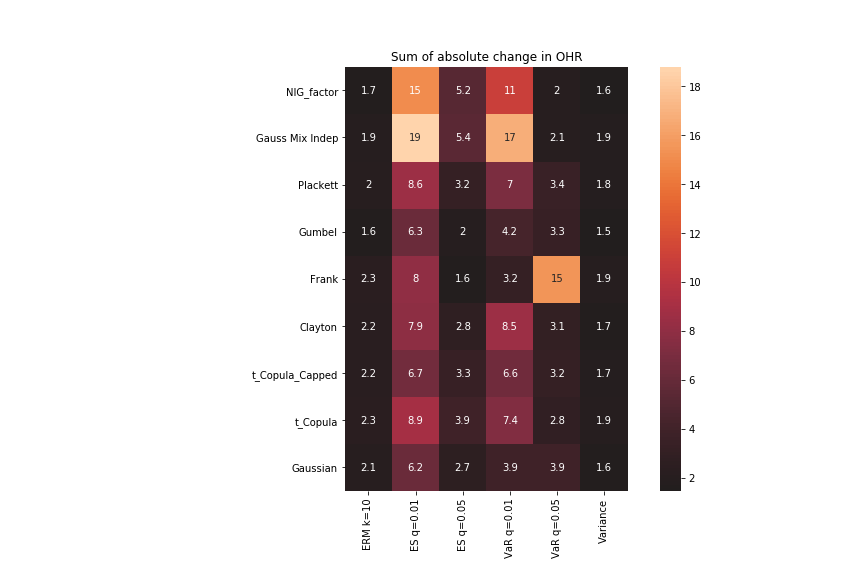
\includegraphics[width=\textwidth]{_pics/Sum of absolute change in OHR.png}
%   \caption{Sum of Absolute Change in OHR.
%   \href{http://www.quantlet.com/}{\includegraphics[width=20pt]{_pics/qletlogo_tr.png}}}
%   \label{fig:SAD}
%\end{figure}

%%! Author = francis
%! Date = 16/08/2021

% Preamble
\documentclass[11pt]{article}

% Packages
\usepackage{amsmath}
\usepackage{array}
\usepackage{booktabs}
\usepackage{caption}


% Document
\begin{document}
\begin{table}[h!]
\begin{center}
\noindent\makebox[\textwidth]{\begin{tabular}{lrrrrrr}
\toprule
{} &       ERM &       ES1 &       ES5 &      VaR1 &      VaR5 &       Var \\
\midrule
copula                       &  0.005824 &  0.017774 &  0.010284 &  0.011473 &  0.006050 &  0.000016 \\
cross hedge                  &  0.005621 &  0.016612 &  0.009939 &  0.010840 &  0.006017 &  0.000015 \\
\% relative diff              &  3.614733 &  6.994292 &  3.477070 &  5.840867 &  0.550620 &  3.673729 \\
spot                         &  0.066608 &  0.190451 &  0.115618 &  0.136746 &  0.063220 &  0.002197 \\
copula in stress period      &  0.005761 &  0.012901 &  0.009832 &  0.010900 &  0.007304 &  0.000015 \\
cross hedge in stress period &  0.005587 &  0.012947 &  0.009621 &  0.010978 &  0.007088 &  0.000015 \\
\% relative diff              &  3.105702 & -0.362275 &  2.198498 & -0.709928 &  3.036827 &  3.462588 \\
spot in stress period        &  0.076401 &  0.155970 &  0.123428 &  0.124419 &  0.097999 &  0.003041 \\
\bottomrule
\end{tabular}
}\end{center}\caption{\label{tab:table0} HE comparison BBT Tiingo}
\end{table}
\begin{table}[h!]
\begin{center}
\noindent\makebox[\textwidth]{\begin{tabular}{lrrrrrr}
\toprule
{} &        ERM &        ES1 &        ES5 &       VaR1 &       VaR5 &        Var \\
\midrule
copula                       &   0.063125 &   0.120135 &   0.092888 &   0.108273 &   0.069064 &   0.002636 \\
cross hedge                  &   0.069192 &   0.148253 &   0.104279 &   0.119498 &   0.077508 &   0.002825 \\
\% relative diff              &  -8.768273 & -18.966206 & -10.923261 &  -9.393743 & -10.894465 &  -6.692165 \\
spot                         &   0.089140 &   0.225694 &   0.144080 &   0.168470 &   0.089899 &   0.004264 \\
copula in stress period      &   0.075088 &   0.125497 &   0.111589 &   0.123216 &   0.092956 &   0.004913 \\
cross hedge in stress period &   0.085074 &   0.176310 &   0.133037 &   0.151116 &   0.097079 &   0.005657 \\
\% relative diff              & -11.737526 & -28.820160 & -16.122014 & -18.462414 &  -4.246979 & -13.154777 \\
spot in stress period        &   0.119040 &   0.250498 &   0.200934 &   0.228042 &   0.156914 &   0.007407 \\
\bottomrule
\end{tabular}
}\end{center}\caption{\label{tab:table1} HE comparison BBT future Tiingo ada}
\end{table}
\begin{table}[h!]
\begin{center}
\noindent\makebox[\textwidth]{\begin{tabular}{lrrrrrr}
\toprule
{} &       ERM &        ES1 &       ES5 &       VaR1 &      VaR5 &       Var \\
\midrule
copula                       &  0.045753 &   0.116154 &  0.071933 &   0.076843 &  0.049148 &  0.001346 \\
cross hedge                  &  0.049662 &   0.130841 &  0.078328 &   0.085429 &  0.050916 &  0.001442 \\
\% relative diff              & -7.871269 & -11.225416 & -8.164547 & -10.050049 & -3.473119 & -6.703109 \\
spot                         &  0.083213 &   0.228328 &  0.142129 &   0.174268 &  0.090164 &  0.003446 \\
copula in stress period      &  0.058527 &   0.169055 &  0.102075 &   0.139861 &  0.064593 &  0.002031 \\
cross hedge in stress period &  0.060755 &   0.178084 &  0.104073 &   0.154476 &  0.062593 &  0.002151 \\
\% relative diff              & -3.667054 &  -5.069882 & -1.919499 &  -9.460939 &  3.195479 & -5.585663 \\
spot in stress period        &  0.100201 &   0.225398 &  0.174061 &   0.178273 &  0.125977 &  0.004865 \\
\bottomrule
\end{tabular}
}\end{center}\caption{\label{tab:table2} HE comparison BBT future Tiingo eth}
\end{table}
\begin{table}[h!]
\begin{center}
\noindent\makebox[\textwidth]{\begin{tabular}{lrrrrrr}
\toprule
{} &       ERM &        ES1 &       ES5 &       VaR1 &      VaR5 &       Var \\
\midrule
copula                       &  0.058828 &   0.149425 &  0.092922 &   0.094752 &  0.063848 &  0.001755 \\
cross hedge                  &  0.062266 &   0.167335 &  0.097900 &   0.110785 &  0.062293 &  0.001813 \\
\% relative diff              & -5.521211 & -10.703020 & -5.085515 & -14.472352 &  2.497494 & -3.216869 \\
spot                         &  0.096164 &   0.261008 &  0.163300 &   0.187398 &  0.095560 &  0.004076 \\
copula in stress period      &  0.067627 &   0.205845 &  0.116784 &   0.113548 &  0.076603 &  0.002621 \\
cross hedge in stress period &  0.068253 &   0.197203 &  0.117779 &   0.117185 &  0.070380 &  0.002617 \\
\% relative diff              & -0.917372 &   4.382310 & -0.845265 &  -3.103126 &  8.841549 &  0.174381 \\
spot in stress period        &  0.113052 &   0.281010 &  0.194193 &   0.185661 &  0.139036 &  0.005688 \\
\bottomrule
\end{tabular}
}\end{center}\caption{\label{tab:table3} HE comparison BBT future Tiingo ltc}
\end{table}
\begin{table}[h!]
\begin{center}
\noindent\makebox[\textwidth]{\begin{tabular}{lrrrrrr}
\toprule
{} &       ERM &       ES1 &       ES5 &      VaR1 &       VaR5 &       Var \\
\midrule
copula                       &  0.079228 &  0.259104 &  0.139501 &  0.151341 &   0.079092 &  0.004273 \\
cross hedge                  &  0.078219 &  0.260633 &  0.139179 &  0.146620 &   0.069081 &  0.004198 \\
\% relative diff              &  1.290945 & -0.586730 &  0.231537 &  3.219567 &  14.492191 &  1.775367 \\
spot                         &  0.095107 &  0.287638 &  0.164290 &  0.179563 &   0.100176 &  0.005283 \\
copula in stress period      &  0.085013 &  0.201083 &  0.147950 &  0.175563 &   0.091099 &  0.005135 \\
cross hedge in stress period &  0.081526 &  0.202907 &  0.143626 &  0.164448 &   0.101811 &  0.004769 \\
\% relative diff              &  4.276966 & -0.898949 &  3.010917 &  6.758591 & -10.521458 &  7.667793 \\
spot in stress period        &  0.094615 &  0.256529 &  0.167473 &  0.201297 &   0.110765 &  0.005255 \\
\bottomrule
\end{tabular}
}\end{center}\caption{\label{tab:table4} HE comparison BBT future Tiingo xrp}
\end{table}
\begin{table}[h!]
\begin{center}
\noindent\makebox[\textwidth]{\begin{tabular}{lrrrrrr}
\toprule
{} &       ERM &       ES1 &       ES5 &      VaR1 &      VaR5 &       Var \\
\midrule
copula                       &  0.012046 &  0.036987 &  0.020541 &  0.020008 &  0.011741 &  0.000096 \\
cross hedge                  &  0.012370 &  0.037775 &  0.021054 &  0.021001 &  0.012867 &  0.000098 \\
\% relative diff              & -2.612613 & -2.084869 & -2.434416 & -4.728842 & -8.752752 & -1.855970 \\
spot                         &  0.066617 &  0.177928 &  0.116244 &  0.142476 &  0.065817 &  0.002086 \\
copula in stress period      &  0.017788 &  0.074821 &  0.036995 &  0.043342 &  0.019570 &  0.000202 \\
cross hedge in stress period &  0.018160 &  0.076033 &  0.037775 &  0.045376 &  0.020252 &  0.000205 \\
\% relative diff              & -2.052817 & -1.594053 & -2.064052 & -4.482996 & -3.369819 & -1.885142 \\
spot in stress period        &  0.080025 &  0.161541 &  0.136882 &  0.145495 &  0.113336 &  0.003409 \\
\bottomrule
\end{tabular}
}\end{center}\caption{\label{tab:table5} HE comparison BBT future BITX}
\end{table}
\begin{table}[h!]
\begin{center}
\noindent\makebox[\textwidth]{\begin{tabular}{lrrrrrr}
\toprule
{} &       ERM &       ES1 &       ES5 &      VaR1 &      VaR5 &       Var \\
\midrule
copula                       &  0.048878 &  0.114332 &  0.077133 &  0.083347 &  0.055215 &  0.001255 \\
cross hedge                  &  0.050137 &  0.119798 &  0.079617 &  0.090130 &  0.053374 &  0.001292 \\
\% relative diff              & -2.512498 & -4.562734 & -3.120502 & -7.525093 &  3.448315 & -2.822839 \\
spot                         &  0.079960 &  0.236711 &  0.131559 &  0.163363 &  0.078888 &  0.003027 \\
copula in stress period      &  0.052494 &  0.202875 &  0.099133 &  0.107227 &  0.063197 &  0.002229 \\
cross hedge in stress period &  0.053169 &  0.210915 &  0.103446 &  0.118473 &  0.061673 &  0.002261 \\
\% relative diff              & -1.268948 & -3.812107 & -4.169720 & -9.492758 &  2.470789 & -1.408455 \\
spot in stress period        &  0.088451 &  0.289595 &  0.173538 &  0.207033 &  0.101460 &  0.005027 \\
\bottomrule
\end{tabular}
}\end{center}\caption{\label{tab:table6} HE comparison BBT future BITW20}
\end{table}
\begin{table}[h!]
\begin{center}
\noindent\makebox[\textwidth]{\begin{tabular}{lrrrrrr}
\toprule
{} &       ERM &       ES1 &       ES5 &      VaR1 &      VaR5 &        Var \\
\midrule
copula                       &  0.054173 &  0.138594 &  0.086839 &  0.084179 &  0.058942 &   0.001696 \\
cross hedge                  &  0.055962 &  0.147383 &  0.090365 &  0.091846 &  0.061897 &   0.001530 \\
\% relative diff              & -3.195267 & -5.963533 & -3.902349 & -8.347861 & -4.774662 &  10.832507 \\
spot                         &  0.085505 &  0.244400 &  0.142102 &  0.177450 &  0.087256 &   0.003382 \\
copula in stress period      &  0.052274 &  0.245347 &  0.110437 &  0.113076 &  0.062958 &   0.003133 \\
cross hedge in stress period &  0.052097 &  0.239297 &  0.110635 &  0.112673 &  0.064207 &   0.002476 \\
\% relative diff              &  0.340950 &  2.528040 & -0.178703 &  0.358032 & -1.945057 &  26.551359 \\
spot in stress period        &  0.093416 &  0.323453 &  0.180239 &  0.199110 &  0.109723 &   0.006061 \\
\bottomrule
\end{tabular}
}\end{center}\caption{\label{tab:table7} HE comparison BBT future BITW70}
\end{table}
\begin{table}[h!]
\begin{center}
\noindent\makebox[\textwidth]{\begin{tabular}{lrrrrrr}
\toprule
{} &       ERM &       ES1 &       ES5 &      VaR1 &      VaR5 &       Var \\
\midrule
copula                       &  0.014238 &  0.047505 &  0.025037 &  0.022217 &  0.014902 &  0.000137 \\
cross hedge                  &  0.014574 &  0.047847 &  0.025399 &  0.022665 &  0.015514 &  0.000140 \\
\% relative diff              & -2.304006 & -0.715975 & -1.424354 & -1.979126 & -3.945876 & -1.798926 \\
spot                         &  0.067329 &  0.186054 &  0.117143 &  0.142941 &  0.065716 &  0.002132 \\
copula in stress period      &  0.020997 &  0.110891 &  0.046718 &  0.053623 &  0.019379 &  0.000324 \\
cross hedge in stress period &  0.021258 &  0.112205 &  0.047341 &  0.053405 &  0.019692 &  0.000329 \\
\% relative diff              & -1.229785 & -1.171451 & -1.314515 &  0.409517 & -1.589530 & -1.326984 \\
spot in stress period        &  0.080456 &  0.197610 &  0.142460 &  0.154426 &  0.110179 &  0.003551 \\
\bottomrule
\end{tabular}
}\end{center}\caption{\label{tab:table8} HE comparison BBT future BITW100}
\end{table}
\begin{table}[h!]
\begin{center}
\noindent\makebox[\textwidth]{\begin{tabular}{lrrrrrr}
\toprule
{} &       ERM &       ES1 &       ES5 &      VaR1 &      VaR5 &       Var \\
\midrule
copula                       &  0.010219 &  0.030425 &  0.017260 &  0.017060 &  0.009533 &  0.000078 \\
cross hedge                  &  0.010083 &  0.031857 &  0.017184 &  0.017522 &  0.009238 &  0.000078 \\
\% relative diff              &  1.347764 & -4.493722 &  0.444115 & -2.635645 &  3.198000 & -0.406715 \\
spot                         &  0.064772 &  0.178374 &  0.114805 &  0.139618 &  0.062770 &  0.001990 \\
copula in stress period      &  0.015169 &  0.068021 &  0.031656 &  0.032183 &  0.016373 &  0.000171 \\
cross hedge in stress period &  0.015036 &  0.071100 &  0.031598 &  0.032708 &  0.016045 &  0.000174 \\
\% relative diff              &  0.884965 & -4.331002 &  0.182983 & -1.606256 &  2.048019 & -1.648355 \\
spot in stress period        &  0.100992 &  0.271385 &  0.173078 &  0.176042 &  0.129120 &  0.004786 \\
\bottomrule
\end{tabular}
}\end{center}\caption{\label{tab:table9} HE comparison BBT future CRIX}
\end{table}
\end{document}




\newpage
\bibliographystyle{abbrvnamed} %
\bibliography{finance} %
\newpage
\appendix
% \section{Appendix}
\section{Density of linear combination of random variables}
\label{sec:appendix}
\begin{proposition}
   Let $\bm{X} = (X_1, ..., X_d)^\top$ be real-valued random variables with corresponding
   copula density $\bm{c}_{X_1, ..., X_d}$, and continuous marginals $F_{X_1}, ..., F_{X_d}$.
   Then, the
   pdf of the linear combination of marginals $Z = n_1 \cdot X_1 +
   ... +  n_d \cdot X_d $ is
   \natp{\em [What does $\circ$ stand for? For functions, always use
     $()$ instead of $\{\}$. Also state that $\mathbf z\in \R$. Use
     the differential operator $\dd$ instead of $d$.]}
   \begin{align}
   f_Z(z) &= \left| n_1^{-1} \right| \int_{[0,1]^{d-1}} \bm{c}_{X_1,...,X_d}
      \{F_{X_1} \circ S(z), u_2, ..., u_d \} \cdot
      f_{X_1} \circ S(z) du_2 ... du_d \label{density} \\
      S(z) &= \frac{1}{n_1}\cdot z - \frac{n_2}{n_1} \cdot F^{(-1)}_{X_2}(u_2) - ... -  \frac{n_d}{n_1} \cdot F^{(-1)}_{X_d}(u_d)
      \end{align}
   \end{proposition}

\begin{proof}
  Rewrite $Z = n_1 \cdot X_1 + ... +  n_d \cdot X_d $ in matrix form
  \natp{\em [Be more precise in the sentence above. The matrix product contains $Z$,
    but it is not equal to $Z$. Instead of defining $\mathbf A$
    implicitly, why not say, let $\mathbf A=...$]}

  \natp{Let $Z= n_1 \cdot X_1 + ... +  n_d \cdot X_d $ and let
    $\mathbf A=\displaystyle \begin{bmatrix}
      n_1    & n_2   & \cdots & n_d     \\
      0      & 1     &  \cdots & 0       \\
      \vdots &       & \ddots & \vdots \\
      0      & \cdots &       & 1  \\
    \end{bmatrix}$. Then,
    \begin{equation*}
      \begin{bmatrix}
        Z \\ X_2 \\ \vdots \\ X_d
      \end{bmatrix}
      = \bm{A}
      \begin{bmatrix}
         X_1 \\ X_2 \\ \vdots \\ X_d
      \end{bmatrix},
    \end{equation*}
    and by a transformation ...
    }
   \begin{align}
      \begin{bmatrix}
      Z \\ X_2 \\ \vdots \\ X_d
      \end{bmatrix}
      = \begin{bmatrix}
      n_1    & n_2   & \cdots & n_d     \\
      0      & 1     &  \cdots & 0       \\
      \vdots &       & \ddots & \vdots \\
      0      & \cdots &       & 1  \\
      \end{bmatrix}
      \begin{bmatrix}
         X_1 \\ X_2 \\ \vdots \\ X_d
      \end{bmatrix}
      = \bm{A}
      \begin{bmatrix}
         X_1 \\ X_2 \\ \vdots \\ X_d
      \end{bmatrix}.
      \end{align} 

   By a transformation of the variables \natp{\em [Where are you taking
     the transformation from, especially as $f$ may be non-linear.]}
   \begin{align}
      \bm{f}_{Z,X_2,...,X_d}(z, x_2, ...,x_d) &= \bm{f}_{X_1,...,X_d}\left( \bm{A}^{-1}
      \begin{bmatrix}
         z \\ x_2 \\ \vdots \\ x_d
      \end{bmatrix}
      \right)  \cdot |\det \bm{A}^{-1}| \\
      &= \left| n_1^{-1} \right| \bm{f}_{X_1,...,X_d}\{S(z), x_2,...,x_d\}
      \end{align} \medskip

   Let $u_i = F_{X_i}(x_i)$ and  use the relationship \natp{\em
     [Provide a reference for this relationship.]}
   \begin{align}
      \bm{c}_{X_1,...,X_d}(u_1, ..., u_d)=\frac{\bm{f}_{X_1,...,X_d}(x_1,...,x_d)}{\prod_{i=1}^d f_{X_i}(x_i)},
   \end{align}
   we have
   \begin{align}
     & \bm{f}_{Z,X_2,...,X_d}(z, x_2, ...,x_d) = \\
      & \left| n_1^{-1} \right| \cdot
      \bm{c}_{X_1,...,X_d}\{F_{X_1} \circ S(z), u_2, ...,  u_d\}  \cdot
      f_{X_1} \{ S(z) \} \cdot
      \prod_{i=2}^d f_{X_i}(x_i)
      \end{align}

   The claim (\ref{density}) is obtained by integrating out $x_2, ... x_d$ by substituting $dx_i = \frac{1}{f_{X_i}(x_i)}du_i$.
   \end{proof}

\clearpage

\section{Summary Statistics of Assets}\begin{table}[th] \centering \resizebox{\textwidth}{!}{%
\begin{tabular}{lrrrrrrrr} \toprule
         {} &    Mean \% &     Std \% &      Skew &       Kurt &         MD \% &     MD date & $\rho$ & $\tau$ \\
\midrule
     \multicolumn{9}{l}{Hedging Instrument} \\
\ \ \ BTCF    &  0.3906 &  4.6312 & -0.5060 &   4.4204 & -26.9920 &  2020-03-12 &  1.0000 &  1.0000 \\
     \multicolumn{9}{l}{Individual Cryptos}                                                                                 \\
\ \ \ BTC     &  0.3915 &  4.4023 & -0.5857 &   4.6565 & -25.9965 &  2020-03-12 &  0.9975 &  0.9507 \\
\ \ \ ETH     &  0.6819 &  6.0103 & -0.2557 &   5.2646 & -32.0144 &  2020-03-12 &  0.7712 &  0.5988 \\
\ \ \ ADA     &  0.9467 &  6.6990 &  0.1661 &   2.3086 & -26.8528 &  2020-03-12 &  0.6296 &  0.4825 \\
\ \ \ LTC     &  0.3227 &  6.4781 & -0.9935 &   5.3011 & -37.5913 &  2021-05-19 &  0.8080 &  0.6113 \\
\ \ \ XRP     &  0.2987 &  7.9843 &  0.5542 &  12.4882 & -52.7652 &  2020-12-23 &  0.4510 &  0.4939 \\
   \multicolumn{9}{l}{Crypto Indices with BTC Constituent}                                                                  \\
\ \ \ BITX    &  0.4308 &  4.5676 & -0.8842 &   4.7222 & -27.0220 &  2020-03-12 &  0.9769 &  0.8738 \\
\ \ \ CRIX    &  0.4602 &  4.5420 & -0.7952 &   4.7549 & -27.1385 &  2020-03-12 &  0.9799 &  0.8769 \\
\ \ \ BITW100 &  0.4683 &  4.6174 & -0.9864 &   4.9381 & -27.2694 &  2020-03-12 &  0.9674 &  0.8537 \\
    \multicolumn{9}{l}{Crypto Indices without BTC Constituent}                                                              \\
\ \ \ BITW20  &  0.6249 &  5.5021 & -1.1518 &   5.2203 & -31.0092 &  2020-03-12 &  0.7674 &  0.5883 \\
\ \ \ BITW70  &  0.6353 &  5.8155 & -1.1171 &   5.1926 & -32.3453 &  2021-05-19 &  0.7525 &  0.5459 \\
\bottomrule
\end{tabular}}
\caption{Summary statistics of assets' daily returns during the out-of-sample period, from 2019-10-21 to 2021-05-27.
        The first four columns are the first four moments of assets' daily returns.
        The fifth and sixth columns are the maximum drawdown (MD) and the date of the MD.
        The last two columns are Pearson's $\rho$s and Kendall's $\tau$s between the assets and BTCF. }
\label{tab:SSA}

\end{table}

\section{Summary Statistics of Hedged Portfolios}\label{sec:SSHP}
\begin{table}[h] \centering \resizebox{\textwidth}{!}{%
\begin{tabular}{lrrrrrrr} \toprule
         {} &    Mean \% &     Std \% &      Skew &       Kurt &         MD \% &     MD date & Variance \\
\midrule
     \multicolumn{7}{l}{Individual Cryptos}                                                                                 \\
\ \ \ BTC     &  0.0215 &  0.3221 & -1.0119 &   3.1929 &  -1.4393 &  2020-11-30 &    0.0000 \\
\ \ \ ETH     &  0.2823 &  3.8741 &  0.9469 &   7.1064 & -17.7421 &  2021-05-19 &    0.0015 \\
\ \ \ ADA     &  0.5617 &  5.2722 &  1.3634 &   4.4818 & -13.8687 &  2021-01-08 &    0.0028 \\
\ \ \ LTC     & -0.0871 &  3.9052 & -0.3617 &   7.6239 & -28.3029 &  2021-05-19 &    0.0018 \\
\ \ \ XRP     & -0.0123 &  7.1537 &  1.1451 &  20.0236 & -52.5236 &  2020-12-23 &    0.0043 \\
   \multicolumn{7}{l}{Crypto Indices with BTC Constituent}                                                                  \\
\ \ \ BITX    &  0.0561 &  0.9954 & -0.4204 &  13.2487 &  -7.7567 &  2021-05-19 &    0.0001 \\
\ \ \ CRIX    &  0.0812 &  0.9183 & -0.0027 &  14.3136 &  -7.1025 &  2021-05-19 &    0.0001 \\
\ \ \ BITW100 &  0.0855 &  1.1986 & -1.7440 &  22.2644 & -11.3866 &  2021-05-19 &    0.0001 \\
    \multicolumn{7}{l}{Crypto Indices without BTC Constituent}                                                              \\
\ \ \ BITW20  &  0.2429 &  3.5846 & -0.3063 &   4.1622 & -21.4680 &  2021-05-19 &    0.0013 \\
\ \ \ BITW70  &  0.2706 &  3.8838 & -0.6490 &   4.6312 & -23.9984 &  2021-05-19 &    0.0015 \\
\bottomrule
\end{tabular}}
\caption{Summary statistics of out-of-sample daily returns of hedged portfolios that minimize variance.}
\label{tab:var_rh}

\end{table}\begin{table}[!] \centering \resizebox{\textwidth}{!}{%
\begin{tabular}{lrrrrrrr} \toprule
         {} &    Mean \% &     Std \% &      Skew &       Kurt &         MD \% &     MD date & VaR 5\% \\
\midrule
     \multicolumn{7}{l}{Individual Cryptos}                                                                                 \\
\ \ \ BTC     &  0.0253 &  0.3294 & -0.9725 &   3.4373 &  -1.5347 &  2020-11-30 &  0.0063 \\
\ \ \ ETH     &  0.3084 &  3.8944 &  1.0243 &   7.4297 & -19.1750 &  2021-05-19 &  0.0514 \\
\ \ \ ADA     &  0.5726 &  5.2204 &  1.2981 &   4.2544 & -14.6974 &  2021-05-19 &  0.0769 \\
\ \ \ LTC     & -0.0742 &  3.9145 & -0.3836 &   7.5384 & -28.3672 &  2021-05-19 &  0.0622 \\
\ \ \ XRP     &  0.0208 &  7.1520 &  1.1269 &  19.8930 & -52.5667 &  2020-12-23 &  0.0683 \\
   \multicolumn{7}{l}{Crypto Indices with BTC Constituent}                                                                  \\
\ \ \ BITX    &  0.0562 &  0.9930 & -0.3117 &  12.4780 &  -7.5639 &  2021-05-19 &  0.0128 \\
\ \ \ CRIX    &  0.0863 &  0.9151 &  0.0718 &  13.7915 &  -6.9744 &  2021-05-19 &  0.0092 \\
\ \ \ BITW100 &  0.0846 &  1.1980 & -1.6592 &  21.3725 & -11.2582 &  2021-05-19 &  0.0164 \\
    \multicolumn{7}{l}{Crypto Indices without BTC Constituent}                                                              \\
\ \ \ BITW20  &  0.2728 &  3.5940 & -0.3721 &   4.4896 & -22.0733 &  2021-05-19 &  0.0546 \\
\ \ \ BITW70  &  0.2847 &  3.9133 & -0.6580 &   4.7874 & -24.6513 &  2021-05-19 &  0.0626 \\
\bottomrule
\end{tabular}}
\caption{Summary statistics of out-of-sample daily returns of hedged portfolios that minimize VaR 5\%.}
\label{tab:VaR5_rh}

\end{table}\begin{table}[!] \centering \resizebox{\textwidth}{!}{%
\begin{tabular}{lrrrrrrr} \toprule
         {} &    Mean \% &     Std \% &      Skew &       Kurt &         MD \% &     MD date & VaR 1\% \\
\midrule
     \multicolumn{7}{l}{Individual Cryptos}                                                                                 \\
\ \ \ BTC     &  0.0176 &  0.3270 & -1.0405 &   3.3742 &  -1.5689 &  2020-11-30 &  0.0134 \\
\ \ \ ETH     &  0.2977 &  3.9132 &  0.9547 &   7.2414 & -18.6061 &  2021-05-19 &  0.1026 \\
\ \ \ ADA     &  0.5562 &  5.3466 &  1.1362 &   3.9334 & -15.4795 &  2021-05-19 &  0.1106 \\
\ \ \ LTC     & -0.0852 &  4.1503 & -0.7234 &   7.3208 & -29.0915 &  2021-05-19 &  0.1030 \\
\ \ \ XRP     &  0.0352 &  7.1658 &  1.1582 &  19.8506 & -52.5727 &  2020-12-23 &  0.1387 \\
   \multicolumn{7}{l}{Crypto Indices with BTC Constituent}                                                                  \\
\ \ \ BITX    &  0.0593 &  1.0178 & -0.5331 &  13.3100 &  -8.0299 &  2021-05-19 &  0.0247 \\
\ \ \ CRIX    &  0.0738 &  0.9695 & -0.4729 &  13.6500 &  -7.0185 &  2021-05-19 &  0.0245 \\
\ \ \ BITW100 &  0.0823 &  1.2338 & -1.9365 &  23.1938 & -11.8752 &  2021-05-19 &  0.0347 \\
    \multicolumn{7}{l}{Crypto Indices without BTC Constituent}                                                              \\
\ \ \ BITW20  &  0.2499 &  3.6210 & -0.3866 &   4.3396 & -21.6634 &  2021-05-19 &  0.0988 \\
\ \ \ BITW70  &  0.2788 &  3.9257 & -0.7635 &   5.1288 & -24.5294 &  2021-05-19 &  0.1147 \\
\bottomrule
\end{tabular}}
\caption{Summary statistics of out-of-sample daily returns of hedged portfolios that minimize VaR 1\%.}
\label{tab:VaR1_rh}

\end{table}\begin{table}[!] \centering \resizebox{\textwidth}{!}{%
\begin{tabular}{lrrrrrrr} \toprule
         {} &    Mean \% &     Std \% &      Skew &       Kurt &         MD \% &     MD date & ES 5\% \\
\midrule
     \multicolumn{7}{l}{Individual Cryptos}                                                                                 \\
\ \ \ BTC     &  0.0204 &  0.3234 & -1.0150 &   3.4423 &  -1.5629 &  2020-11-30 &  0.0101 \\
\ \ \ ETH     &  0.3082 &  3.8890 &  1.0119 &   7.4077 & -18.7819 &  2021-05-19 &  0.0782 \\
\ \ \ ADA     &  0.5525 &  5.2673 &  1.2557 &   4.2423 & -14.9647 &  2021-05-19 &  0.0984 \\
\ \ \ LTC     & -0.0808 &  3.9829 & -0.4957 &   7.2302 & -28.4608 &  2021-05-19 &  0.0962 \\
\ \ \ XRP     &  0.0176 &  7.1533 &  1.1411 &  19.9176 & -52.5698 &  2020-12-23 &  0.1354 \\
   \multicolumn{7}{l}{Crypto Indices with BTC Constituent}                                                                  \\
\ \ \ BITX    &  0.0591 &  1.0065 & -0.3453 &  12.1335 &  -7.6211 &  2021-05-19 &  0.0215 \\
\ \ \ CRIX    &  0.0777 &  0.9207 &  0.0164 &  13.5608 &  -6.9894 &  2021-05-19 &  0.0173 \\
\ \ \ BITW100 &  0.0848 &  1.2125 & -1.6397 &  19.7472 & -11.1357 &  2021-05-19 &  0.0274 \\
    \multicolumn{7}{l}{Crypto Indices without BTC Constituent}                                                              \\
\ \ \ BITW20  &  0.2608 &  3.6115 & -0.3555 &   4.2016 & -21.5430 &  2021-05-19 &  0.0804 \\
\ \ \ BITW70  &  0.2785 &  3.9157 & -0.6949 &   4.8047 & -24.3474 &  2021-05-19 &  0.0908 \\
\bottomrule
\end{tabular}}
\caption{Summary statistics of out-of-sample daily returns of hedged portfolios that minimize ES 5\%.}
\label{tab:ES5_rh}

\end{table}\begin{table}[!] \centering \resizebox{\textwidth}{!}{%
\begin{tabular}{lrrrrrrr} \toprule
         {} &    Mean \% &     Std \% &      Skew &       Kurt &         MD \% &     MD date & ES 1\% \\
\midrule
     \multicolumn{7}{l}{Individual Cryptos}                                                                                 \\
\ \ \ BTC     &  0.0148 &  0.3476 & -0.8354 &   3.3054 &  -1.6225 &  2020-11-30 &  0.0234 \\
\ \ \ ETH     &  0.3080 &  3.8954 &  0.9840 &   7.4947 & -18.7625 &  2021-05-19 &  0.1299 \\
\ \ \ ADA     &  0.5016 &  5.4040 &  1.1008 &   3.9607 & -15.4481 &  2021-05-19 &  0.1463 \\
\ \ \ LTC     & -0.1029 &  4.1581 & -0.7757 &   7.4375 & -29.1727 &  2021-05-19 &  0.1647 \\
\ \ \ XRP     & -0.0200 &  7.2887 &  1.1121 &  18.8732 & -52.5700 &  2020-12-23 &  0.2516 \\
   \multicolumn{7}{l}{Crypto Indices with BTC Constituent}                                                                  \\
\ \ \ BITX    &  0.0598 &  1.0312 & -0.4410 &  11.5863 &  -7.7424 &  2021-05-19 &  0.0411 \\
\ \ \ CRIX    &  0.0835 &  0.9461 & -0.0361 &  12.4047 &  -7.0203 &  2021-05-19 &  0.0350 \\
\ \ \ BITW100 &  0.0781 &  1.2640 & -1.9645 &  21.8836 & -11.9263 &  2021-05-19 &  0.0593 \\
    \multicolumn{7}{l}{Crypto Indices without BTC Constituent}                                                              \\
\ \ \ BITW20  &  0.2538 &  3.6323 & -0.4086 &   4.4462 & -21.9866 &  2021-05-19 &  0.1282 \\
\ \ \ BITW70  &  0.2660 &  3.9320 & -0.7598 &   5.0050 & -24.4764 &  2021-05-19 &  0.1535 \\
\bottomrule
\end{tabular}
}
\caption{Summary statistics of out-of-sample daily returns of hedged portfolios that minimize ES 1\%.}
\label{tab:ES1_rh}

\end{table}\begin{table}[!] \centering \resizebox{\textwidth}{!}{%
\begin{tabular}{lrrrrrrr} \toprule
         {} &    Mean \% &     Std \% &      Skew &       Kurt &         MD \% &     MD date & ERM k=10 \\
\midrule
     \multicolumn{7}{l}{Individual Cryptos}                                                                                 \\
\ \ \ BTC     &  0.0223 &  0.3221 & -1.0008 &   3.4153 &  -1.5242 &  2020-11-30 &    0.0057 \\
\ \ \ ETH     &  0.3117 &  3.8679 &  1.0345 &   7.5751 & -18.8729 &  2021-05-19 &    0.0491 \\
\ \ \ ADA     &  0.5722 &  5.3590 &  1.4203 &   4.6970 & -14.3885 &  2021-01-08 &    0.0700 \\
\ \ \ LTC     & -0.0512 &  3.8812 & -0.2929 &   7.7022 & -28.0879 &  2021-05-19 &    0.0616 \\
\ \ \ XRP     &  0.0155 &  7.1579 &  1.1244 &  19.8583 & -52.5689 &  2020-12-23 &    0.0787 \\
   \multicolumn{7}{l}{Crypto Indices with BTC Constituent}                                                                  \\
\ \ \ BITX    &  0.0590 &  1.0078 & -0.4427 &  13.0839 &  -7.8581 &  2021-05-19 &    0.0127 \\
\ \ \ CRIX    &  0.0840 &  0.9087 &  0.0488 &  14.5501 &  -7.0530 &  2021-05-19 &    0.0100 \\
\ \ \ BITW100 &  0.0853 &  1.2032 & -1.6522 &  20.5562 & -11.1846 &  2021-05-19 &    0.0153 \\
    \multicolumn{7}{l}{Crypto Indices without BTC Constituent}                                                              \\
\ \ \ BITW20  &  0.2564 &  3.6009 & -0.3446 &   4.2152 & -21.5920 &  2021-05-19 &    0.0503 \\
\ \ \ BITW70  &  0.2818 &  3.9074 & -0.6952 &   4.8745 & -24.5250 &  2021-05-19 &    0.0557 \\
\bottomrule
\end{tabular}}
\caption{Summary statistics of out-of-sample daily returns of hedged portfolios that minimize ERM $k=10$.}
\label{tab:ERM_rh}

\end{table}


%\newpage
%\begin{landscape}
%\begin{figure}[h]
%   \centering
%   \includegraphics[width=\linewidth]{_pics/Rhs.pdf}
%   \caption{Out-of-Sample Returns of Hedged Portfolio of Copulas and Risk Reduction Objectives.
%   \href{http://www.quantlet.com/}{\includegraphics[width=20pt]{_pics/qletlogo_tr.png}}}
%   \label{fig:OOSRH}
%\end{figure}
%\end{landscape}
%\newpage
%
%\newpage
%\begin{landscape}
%\begin{figure}[th]
%   \centering
%   \includegraphics[width=\linewidth]{_pics/OHRs.pdf}
%   \caption{Optimal Hedge Ratio Obtained from Combinations of Copula and Risk Reduction Objective.
%   \href{http://www.quantlet.com/}{\includegraphics[width=20pt]{_pics/qletlogo_tr.png}}}
%   \label{fig:OHRs}
%\end{figure}
%\end{landscape}
%\newpage


%\section{Data}\label{subsec:data}
In the empirical analysis, we consider the risk reduction capability of the BTC-future (BTCF) on five cryptos
, BTC, ETH, ADA, LTC, and XRP, and five crypto indexes, BITX, BITW100, CRIX, BITW20, and BITW70,
For each of the 10 hedging portfolios, a crypto or index is considered as the spot and held in a unit size long position,
and the BTCF is held in short position of OHR unit in order to reduce the risk of the spot.
All the hedging portfolios are cross asset hedging except the BTCF portfolio.
ETH, ADA, LTC, and XRP are popular cryptos tradable in various exchanges and have large market capitalization.
BITX, BITW100, and CRIX are market-cap weighted crypto indexes with BTC as constituent.
BITX and BITW100 tracks the total return of the 10 and 100 cryptos with largest market-cap respectively.
CRIX decides the number of constituents by AIC and track that number of cryptos with largest market-cap.
In our case, the number of constituents in CRIX is 5.
BITW20 is also a market-cap weighted crypto index but with 20 largest market-cap cryptos outside the constituents of
BITX.
BITW70 has the same construction as BITW20 but with 70 largest market-cap cryptos outside BITX and BITW20.
Therefore, BTC is excluded as constituent in BITW20 and BITW70. \medskip

We collect the spots' and BTCF's daily price at 15:00 US Central Time (CT).
The reason of choosing this particular time is that the CME group determines the daily settlements for BTCFs based on the trading activities on CME Globex between 14:59 and 15:00 CT.
15:00 CT is also the reporting time of the daily closing price by the Bloomberg Terminal (BBT).
Cryptos data are collected from a data provider called Tiingo.
Tiingo aggregates crypto OHLC (open, high, low, and close) prices fed by APIs from various exhcanges.
Tiingo covers major exchanges, e.g. Binance, Gemini, Poloniex etc., so Tiingo's aggregated OHLC price is a good representation a market tradable price.
For each crypto, we match the opening price at 15:00 CT from Tiingo with the daily closing price of BTCF from BBT.
Since CRIX is not available at 15:00 CT, we recalculate a hourly CRIX using the monthly constituents weights and the hourly OHLC price data collected from Tiingo.
BITX, BITW20, BITW70, and BITW100 are collected from the official website of their publisher Bitwise.com.
The daily reporting time of the Bitwise indexes is 15:00 CT. \medskip

At the time of writing, the CRIX' is undergoing the listing process on the S\&P Dow Jones Indices,
the official CRIX data will then be calculated with Lukka Prime Data and available to public via S\&P.



















%\francis{\em This section is under construction}
%Cryptocurrenices are traded around the clock, but CME future are traded from
%Sunday to Friday from 05:00 p.m. to 04:00 p.m. U.S. central time.
%We match the timestamps and timezones of different data sources.
%
%
%\begin{table}[htbp]
%    \centering
%    \begin{tabularx}{\textwidth}{s|CCCCCCCC}
%      \hline\hline
%     \# & Asset & Data Source & Type & Tradable at CT\footnotemark & Tradable at CET\footnotemark during CST\footnotemark & Tradable at CET during CDT\footnotemark & Tradable at UTC during CST & Tradable at UTC during CDT\\       \hline
%      1 & Bitcoin & Coingecko API & Hourly Close &  & 11:00pm D+0 & 11:00pm D+0 & 10:00pm D+0$^*$ &10:00pm D+0$^*$ \\\hline
%      2 & CME Future & Bloomberg & Daily Open & 05:00pm D-1 & 00:00am D+0$^*$ & 00:00am D+0$^*$ & 11:00pm D-1 & 10:00pm D-1 \\       \hline
%      3 & CME Future & Bloomberg & Daily Close & 04:00pm D+0& 11:00pm D+0$^*$ & 11:00pm D+0$^*$ & 10:00pm D+0 & 09:00pm D+0\\       \hline
%      4 & CRIX & IRTG (from Coingecko) & Index &  &  &  & & 00:00am D+0$^*$\\\hline
%    \end{tabularx}
%    \caption{$^*$ indicates the timestamp of raw data from data source. }
%    \label{tab:table}
%\end{table}
%
%\addtocounter{footnote}{-3}
%\footnotetext{CT stands for U.S. Central Time. It represents two observances of time, the Central Standard Time (CST) and the Central Daylight Time (CDT)}
%\addtocounter{footnote}{1}
%\footnotetext{CET stands for Central European Time. It is one hour ahead UTC.}
%\addtocounter{footnote}{1}
%\footnotetext{CST is six hours behind UTC.}
%\addtocounter{footnote}{1}
%\footnotetext{CDT is five hours behind UTC.}
%
%Hedging Pair 1 is hedging \#1 (Bitcoin Spot) with \#3 (CME future).
%The time difference between the two prices is zero.
%They are both adjusted to CET time:
%\#1 by pandas.Series.dt.tz\_convert; \#3 by retrieving data from Bloomberg Terminal located in Berlin. \medskip
%
%Hedging Pair 2 is hedging \#4 (CRIX) with \#2 (CME future).
%We observe \#2 two hours and one hour before \#4 during CST and CDT respectively.
%
%
%\subsection{Time Difference}\label{subsec:time-difference}
%\begin{table}[h]
%    \centering
%
%\begin{tabular}{lrrrr}
%\toprule
%{} &     Open &     High &      Low &    Close \\
%\midrule
%2021-02-02 23:00 &  36360.0 &  38155.0 &  36240.0 &  37790.0 \\
%2021-02-01 23:00 &  34205.0 &  36665.0 &  34070.0 &  36535.0 \\
%2021-01-31 23:00 &  33715.0 &  35280.0 &  32800.0 &  34265.0 \\
%2021-01-28 23:00 &  33995.0 &  39530.0 &  32590.0 &  35180.0 \\
%2021-01-27 23:00 &  31005.0 &  33710.0 &  30350.0 &  33085.0 \\
%\bottomrule
%\end{tabular}
%       \caption{CME Bitcoin Future Raw Data}
%    \label{tab:table0} \medskip
%
%    \begin{tabular}[width=\textwidth]{llrrrr}
%\toprule
% &                      date &           CRIX &   future &  log return CRIX &  log return future \\
%\midrule
%0 & 2021-02-04  &  104518.468839 &  38080.0 &         0.054757 &           0.046220 \\
%1 & 2021-02-03  &   98949.179255 &  36360.0 &         0.059741 &           0.061097 \\
%2 & 2021-02-02  &   93210.948461 &  34205.0 &         0.002204 &           0.014429 \\
%3 & 2021-02-01  &   93005.711051 &  33715.0 &         0.013628 &          -0.008271 \\
%4 & 2021-01-29  &   91746.863103 &  33995.0 &         0.081917 &           0.092065 \\
%\bottomrule
%    \end{tabular}
%    \caption{CRIX \#4 with Opening price of CME Bitcoin future \#2 and their log returns}
%    \label{tab:table2} \medskip
%
%\begin{tabular}{llrrrr}
%\toprule
%{} &                      date &           CRIX &   future &  log return CRIX &  log return future \\
%\midrule
%0 & 2021-02-05  &  103348.488555 &  38220.0 &        -0.011257 &           0.011314 \\
%1 & 2021-02-04  &  104518.468839 &  37790.0 &         0.054757 &           0.033774 \\
%2 & 2021-02-03  &   98949.179255 &  36535.0 &         0.059741 &           0.064146 \\
%3 & 2021-02-02  &   93210.948461 &  34265.0 &        -0.016175 &          -0.026353 \\
%4 & 2021-01-30  &   94730.919657 &  35180.0 &         0.032007 &           0.061398 \\
%\bottomrule
%\end{tabular}
%    \caption{CRIX \#4 with Closing price of CME Bitcoin future \#3 shifted for one day (D-1) and their log returns}
%    \label{tab:table3}
%\end{table}
%
%\clearpage
%\begin{figure}[ht]
%    \centering
%    \includegraphics[scale=.35]{_pics_notes/CRIX_future_Open_Close.pdf}
%    \end{figure}
%
%Kendall's tau between CRIX and future Close is 0.608429;\\
%Kendall's tau between CRIX and future Open is 0.673266; we pick this unless we have hourly CRIX.
%
%\subsection{Statistics of Percentage Difference Between CME Bitcoin future Open Price and Last Close Price}
%
%$$\text{diff} = \frac{\text{Open}_{t} - \text{Close}_{t-1}} {\text{Close}_{t-1}}$$
%
%Mean of diff = 0.00236\\
%Std of diff = 0.02206\\
%Max of diff = 0.16394 \\
%UQ of diff = 0.00814 \\
%Median of diff = 0.00132\\
%LQ of diff = -0.00412 \\
%Min of diff = -0.12190 \\




%%% Local Variables:
%%% mode: latex
%%% TeX-master: "SRM"
%%% End:


\end{document}
